%-----------------------------------------------------------------------------------------------%
%
% Maret 2019
% Template Latex untuk Tugas Akhir Program Studi Sistem informasi ini
% dikembangkan oleh Inggih Permana (inggihjava@gmail.com)
%
% Template ini dikembangkan dari template yang dibuat oleh Andreas Febrian (Fasilkom UI 2003).
%
% Orang yang cerdas adalah orang yang paling banyak mengingat kematian.
%
%-----------------------------------------------------------------------------------------------%

%-----------------------------------------------------------------------------%
\chapter{\babLima}
%-----------------------------------------------------------------------------%

%-----------------------------------------------------------------------------%
\section{Hasil Implementasi}
%-----------------------------------------------------------------------------%
Setelah tahapan dari analisa serta perancangan selesai dilaksanakan maka dilanjutkan ke tahapan dari implementasi dan pengujian. 
Adapun tahapan ini dilakukan pengujian terhadap fitur-fitur yang tersedia pada aplikasi, selanjutnya dilakukan pengamatan dari hasil pengujian tersebut sehingga diketahui fitur-fitur yang masih memiliki kekurangan untuk diambil kesimpulan. Pengujian aplikasi ini menggunakan perangkat PC atau Laptop


\subsection{Lingkungan Implementasi}

Tahap Implmentasi dan pengujian pada sistem surat ini di lakukan terhadap perangkat keras dan perangkat lunak sebagai berikut :
\begin{enumerate}
	\item \textbf{Lingkungan Perangkat lunak}.
	
	Perangkat keras yang digunakan dalam implementasi sistem surat adalah sebagai berikut :
	
	\begin{enumerate}
		\item \textit{Operating System} : Windows 10.
		\item  Bahasa Pemrograman: \textit{CodeIgniter}, dan SQL.
		\item \textit{Web Browser}: Mozilla Firefox dan Google Chroom.
		\item Tools Pengembangan: \textit{Vscode Text Editor}.
		\item \textit{Server}: \textit{XAMPP}.
		\item Pemodelan UML: \textit{Microsoft Visio 2019}.
		\item \textit{Desaign Tools} : Balsamiq Mockup
	\end{enumerate}
	
	\item \textbf{Lingkungan Perangkat Keras}
	\begin{enumerate}
		\item \textit{Processor} : Intel(R) Core(TM) i5-8250u CPU @ 1.6GHz.
		\item \textit{RAM} : 8GB
		\item \textit{SSD} : 256GB
	\end{enumerate}
\end{enumerate}

%-----------------------------------------------------------------------------%
\subsection{Hasil Implementasi}
%-----------------------------------------------------------------------------%
Hasil Implementasi yang dilakukan akan ditampilkan pada sub-bab ini. berikut adalah tampilan awal dari sistem surat  \pic~\ref{loginpage} :
\begin{figure}
	\centering
	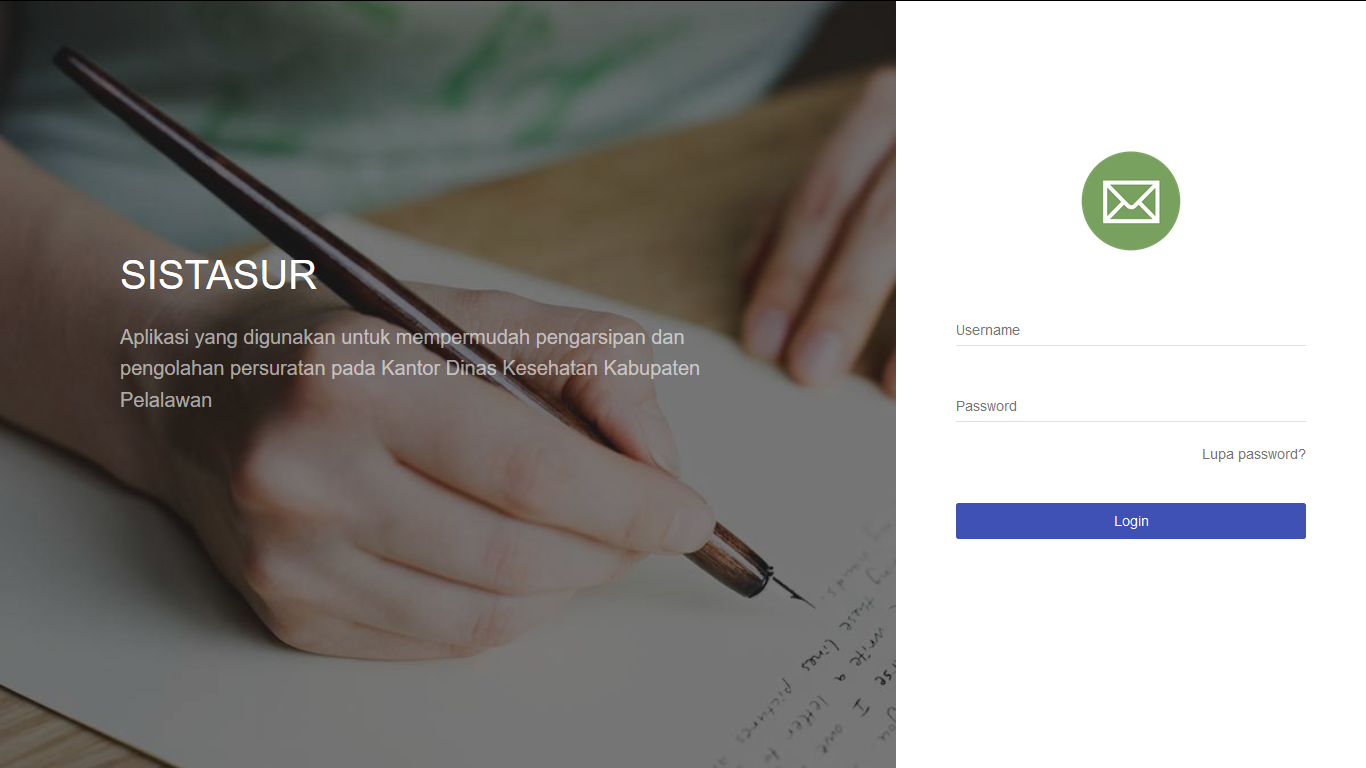
\includegraphics[height= 7cm, width=11cm]{konten/gambar/UISistemSurat/0.0.LoginPage.png}
	\caption{Tampilan Halaman \textit{Login}}
	\label{loginpage}
\end{figure}

dan berikut merupakan tampilan halaman sistem sesuai \textit{role} akses masing - masing :

\begin{enumerate}
	\item \textbf{Admin}
	
	berikut adalah tampilan dari sisi admin
	
	\begin{enumerate}
		\item Dashboard
		
		Berikut adalah tampilan untuk melihat Dashboard dapat dilihat pada \pic~\ref{HalamanDashboard}
		
		\begin{figure}
			\centering
			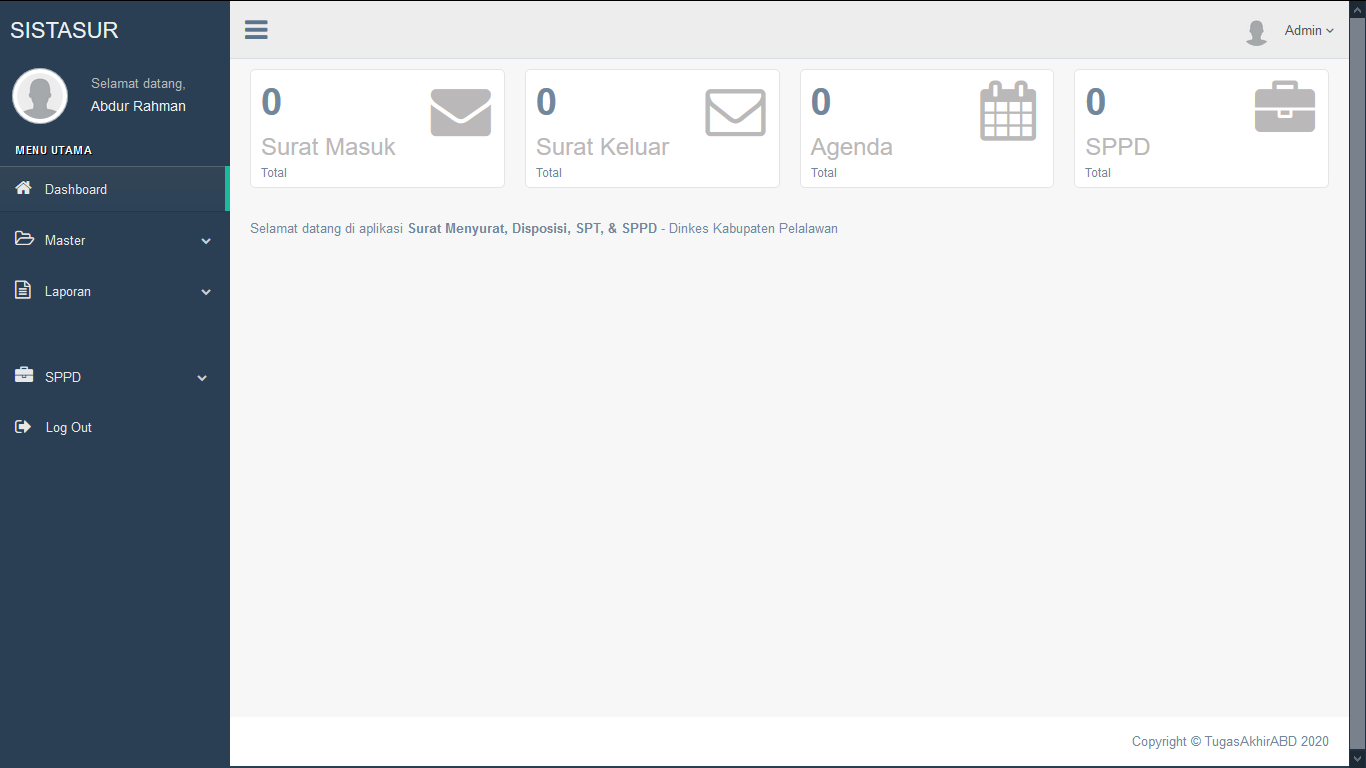
\includegraphics [height= 7cm, width=11cm]{konten/gambar/UISistemSurat/Admin/0.1.Dashboard.png}
			\caption{Halaman Dashboard}
			\label{HalamanDashboard}
		\end{figure}
		
		\item Edit Profil Admin
		
		Berikut adalah tampilan untuk mengakses Halaman Edit Profil Admin dapat dilihat pada \pic~\ref{HalamanEditProfilAdmin}
		
		\begin{figure}
			\centering
			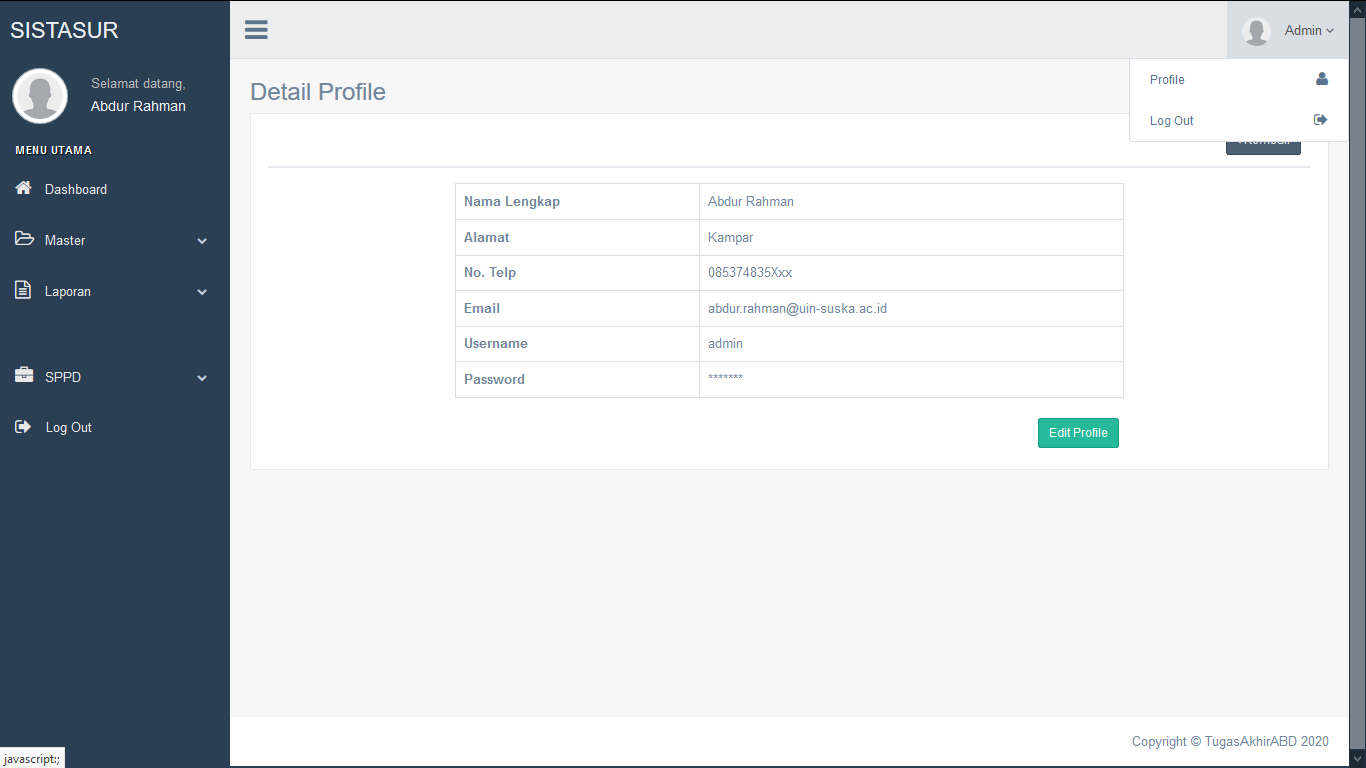
\includegraphics [height= 7cm, width=11cm]{konten/gambar/UISistemSurat/Admin/1.1.DetailProfile.png}
			\caption{Halaman Edit Profil}
			\label{HalamanEditProfilAdmin}
		\end{figure}
		
		\item Lihat Data Golongan Pegawai
		
		Berikut adalah tampilan untuk mengakses Halaman Data Golongan Pegawai dapat dilihat pada \pic~\ref{LihatDataGolonganPegawai}
		
		\begin{figure}
			\centering
			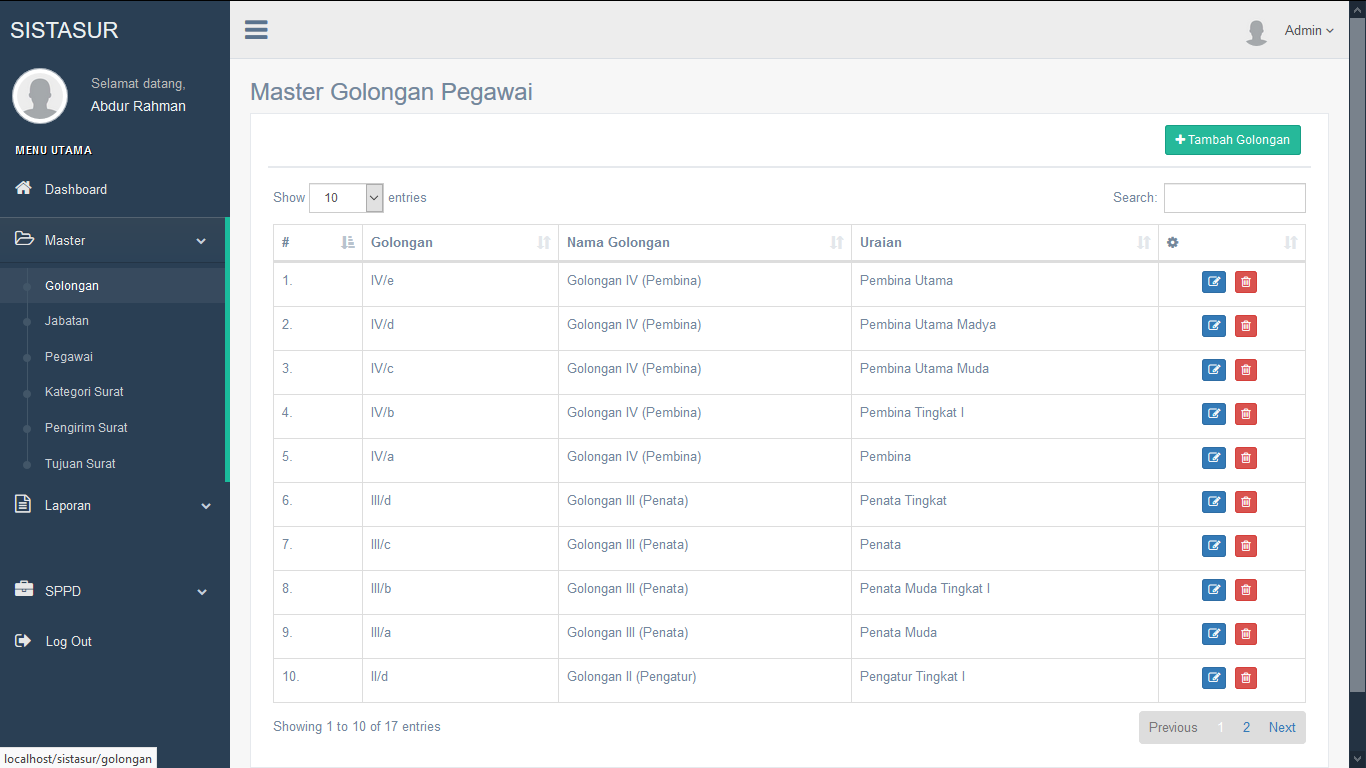
\includegraphics [height= 7cm, width=11cm]{konten/gambar/UISistemSurat/Admin/2.LihatDataGolonganPegawai.png}
			\caption{Lihat Data Golongan Pegawai}
			\label{LihatDataGolonganPegawai}
		\end{figure}
		
		\item Input Data Golongan Pegawai
		
		Berikut adalah tampilan untuk mengakses Halaman Menginput Data Golongan Pegawai dapat dilihat pada  \pic~\ref{InputDataGolonganPegawai}
		
		\begin{figure}
			\centering
			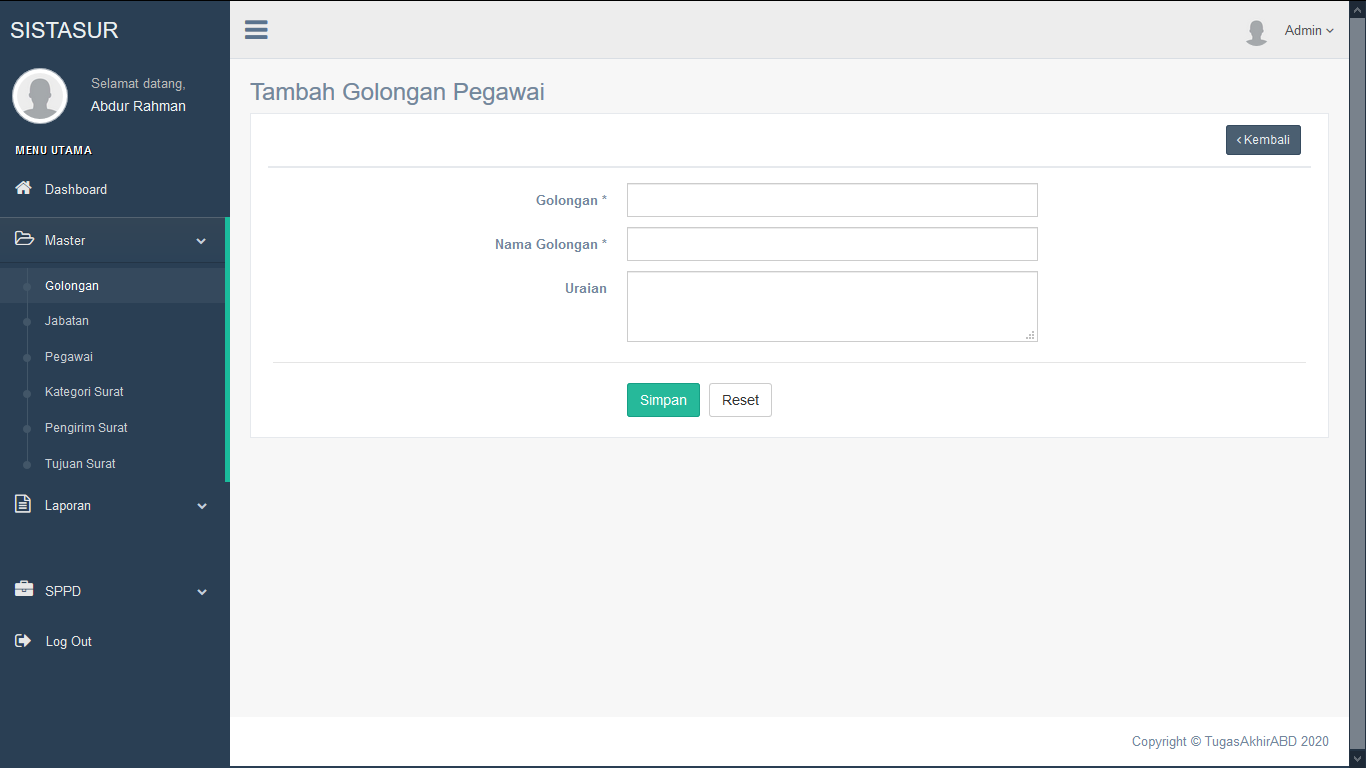
\includegraphics [height= 7cm, width=11cm]{konten/gambar/UISistemSurat/Admin/3.InputDataGolonganPegawai.png}
			\caption{Input Data Golongan Pegawai}
			\label{InputDataGolonganPegawai}
		\end{figure}
		
		\item Lihat Master Jabatan Pegawai
		
		Berikut adalah tampilan untuk mengakses Halaman Melihat Master Jabatan Pegawai dapat dilihat pada \pic~\ref{lihatMasterJabatanPegawai}
		
		\begin{figure}
			\centering
			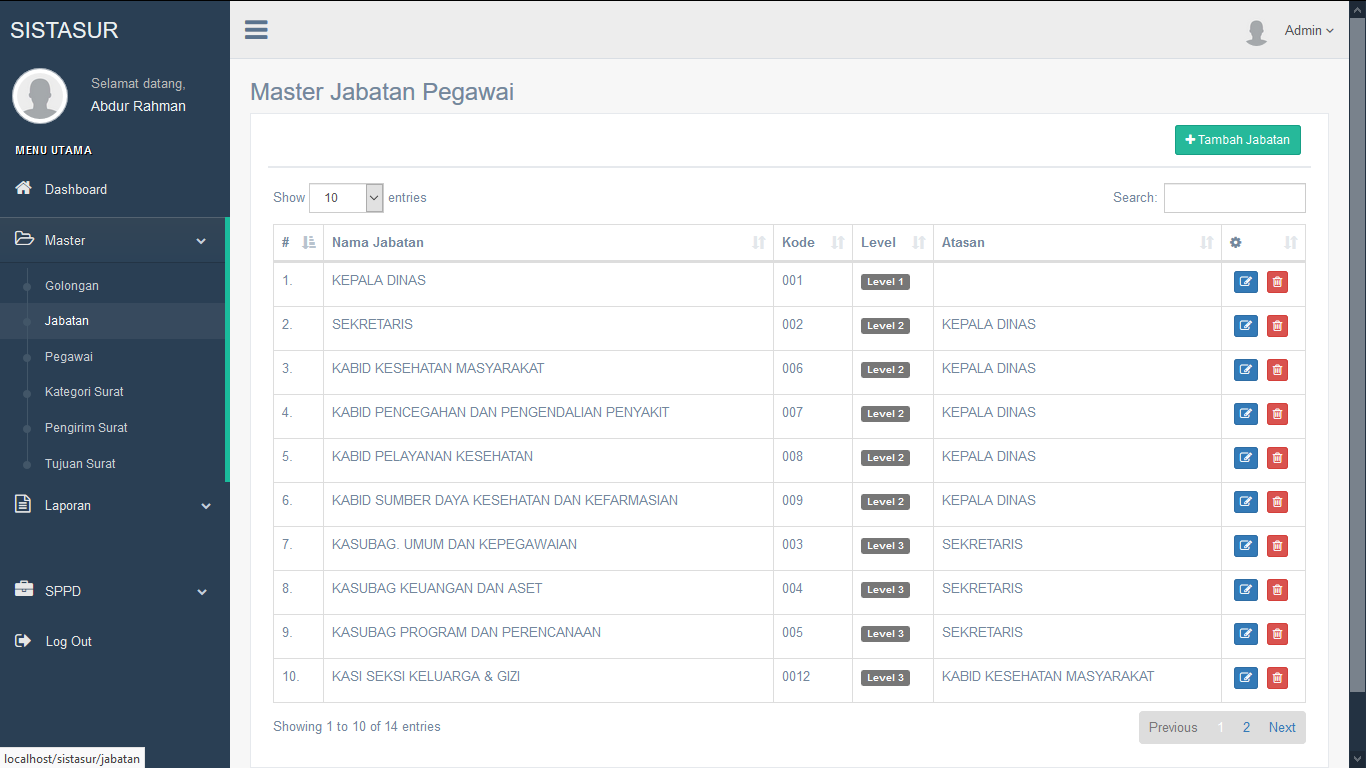
\includegraphics [height= 7cm, width=11cm]{konten/gambar/UISistemSurat/Admin/4.lihatMasterJabatanPegawai.png}
			\caption{Lihat Master Jabatan Pegawai}
			\label{lihatMasterJabatanPegawai}
		\end{figure}
		
		\item Tambah Data Jabatan Pegawai
		
		Berikut adalah tampilan untuk mengakses Menambah Data Jabatan Pegawai dapat dilihat pada \pic~\ref{TambahDataJabatanPegawai}
		
		\begin{figure}
			\centering
			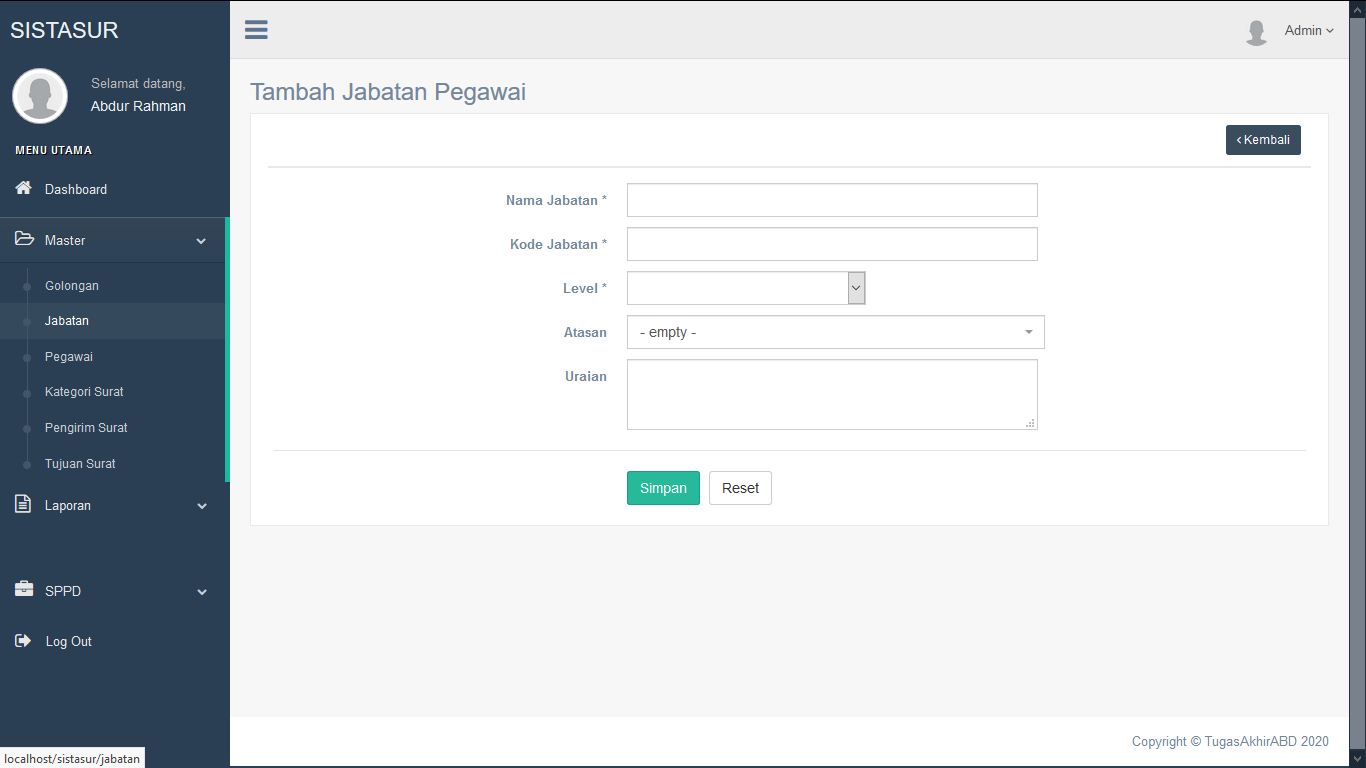
\includegraphics [height= 7cm, width=11cm]{konten/gambar/UISistemSurat/Admin/5.TambahDataJabatanPegawai.png}
			\caption{Tambah Data Jabatan Pegawai}
			\label{TambahDataJabatanPegawai}
		\end{figure}	
		
		\item Tambah Data Pegawai
		
		Berikut adalah tampilan Menambah data pegawai dapat dilihat pada \pic~\ref{TambahDataPegawai}
		
		\begin{figure}
			\centering
			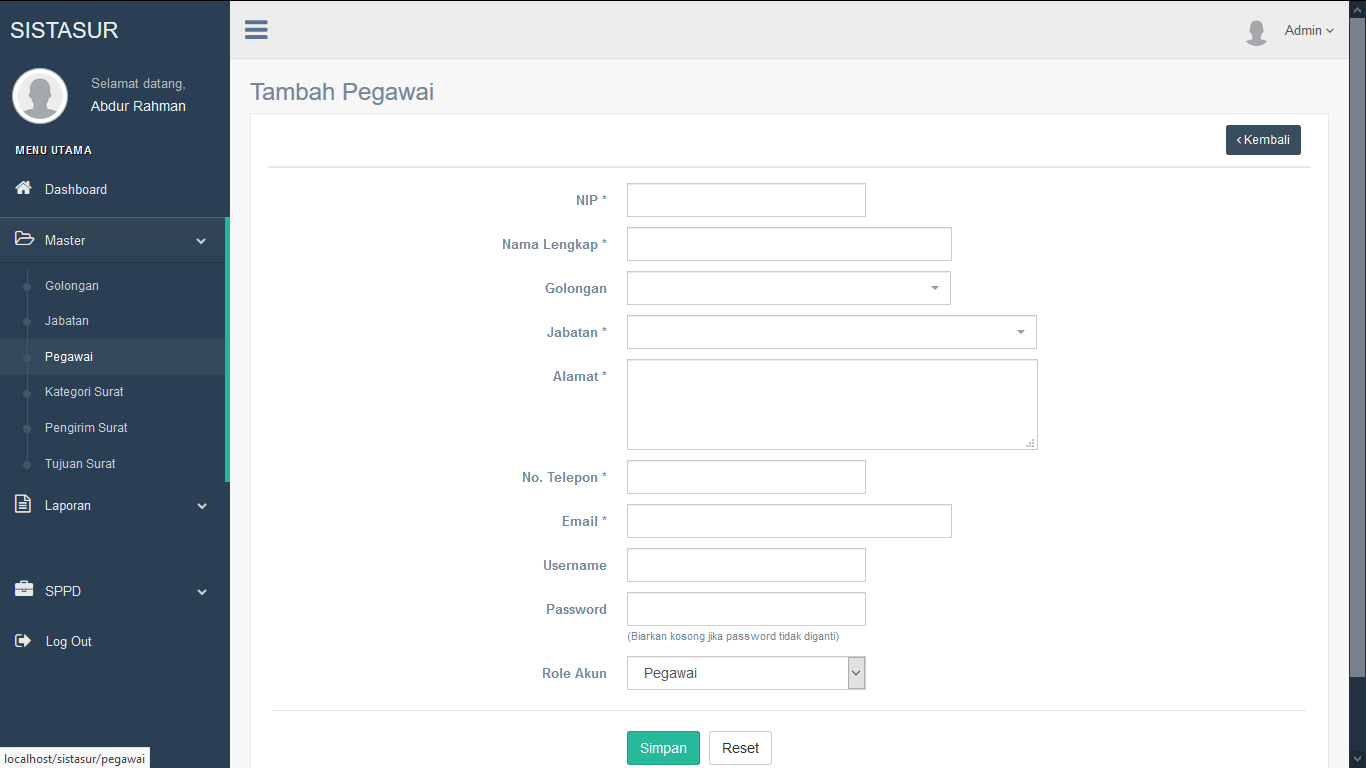
\includegraphics [height= 7cm, width=11cm]{konten/gambar/UISistemSurat/Admin/6.TambahDataPegawai.png}
			\caption{Tambah Data Pegawai}
			\label{TambahDataPegawai}
		\end{figure}
		
		\item Lihat Struktur Organisasi
		
		Berikut adalah tampilan Melihat Struktur Organisasi dapat dilihat pada \pic~\ref{LihatStrukturOrganisasi}
		
		\begin{figure}
			\centering
			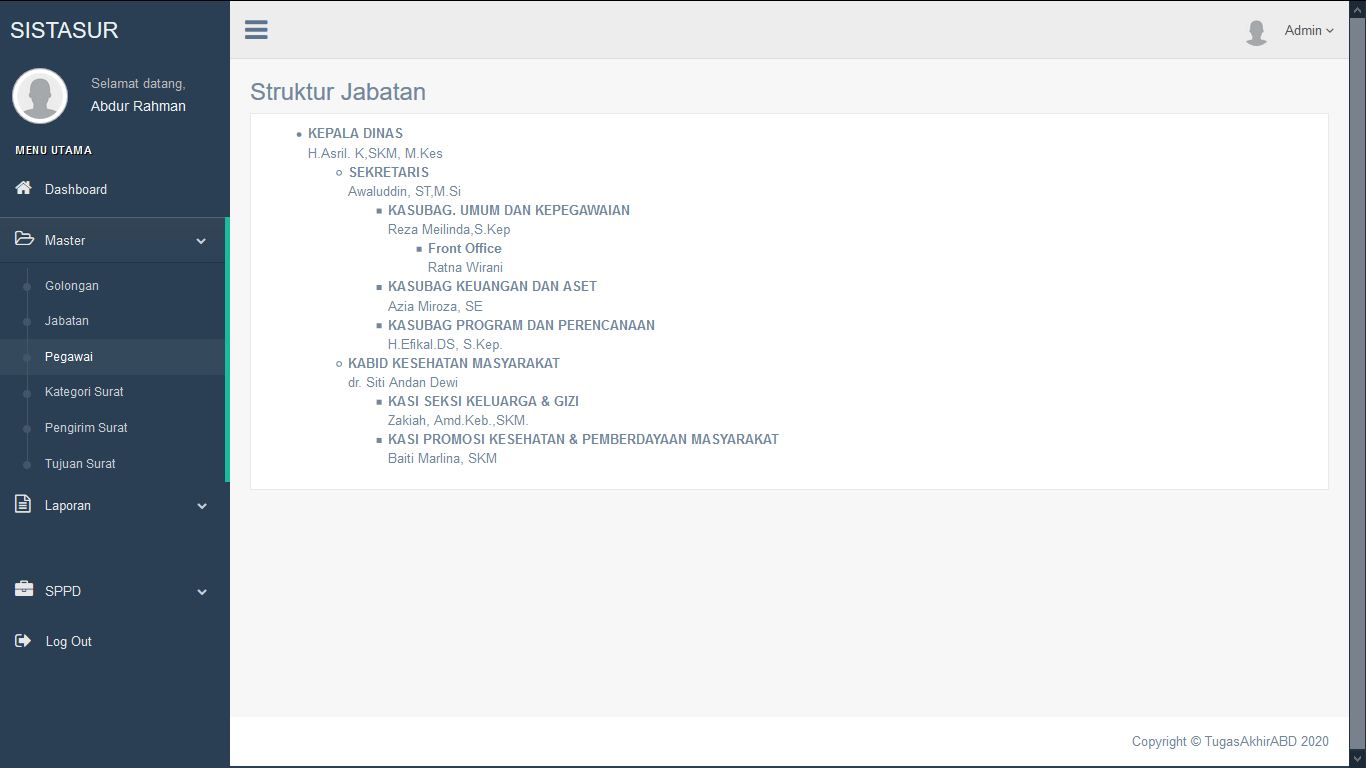
\includegraphics [height= 7cm, width=11cm]{konten/gambar/UISistemSurat/Admin/7.LihatStrukturOrganisasi.png}
			\caption{Lihat Struktur Organisasi}
			\label{LihatStrukturOrganisasi}
		\end{figure}
		
		\item Lihat Kategori Surat
		
		Berikut adalah tampilan Melihat Kategori Surat dapat dilihat pada \pic~\ref{LihatKategoriSurat}
		
		\begin{figure}
			\centering
			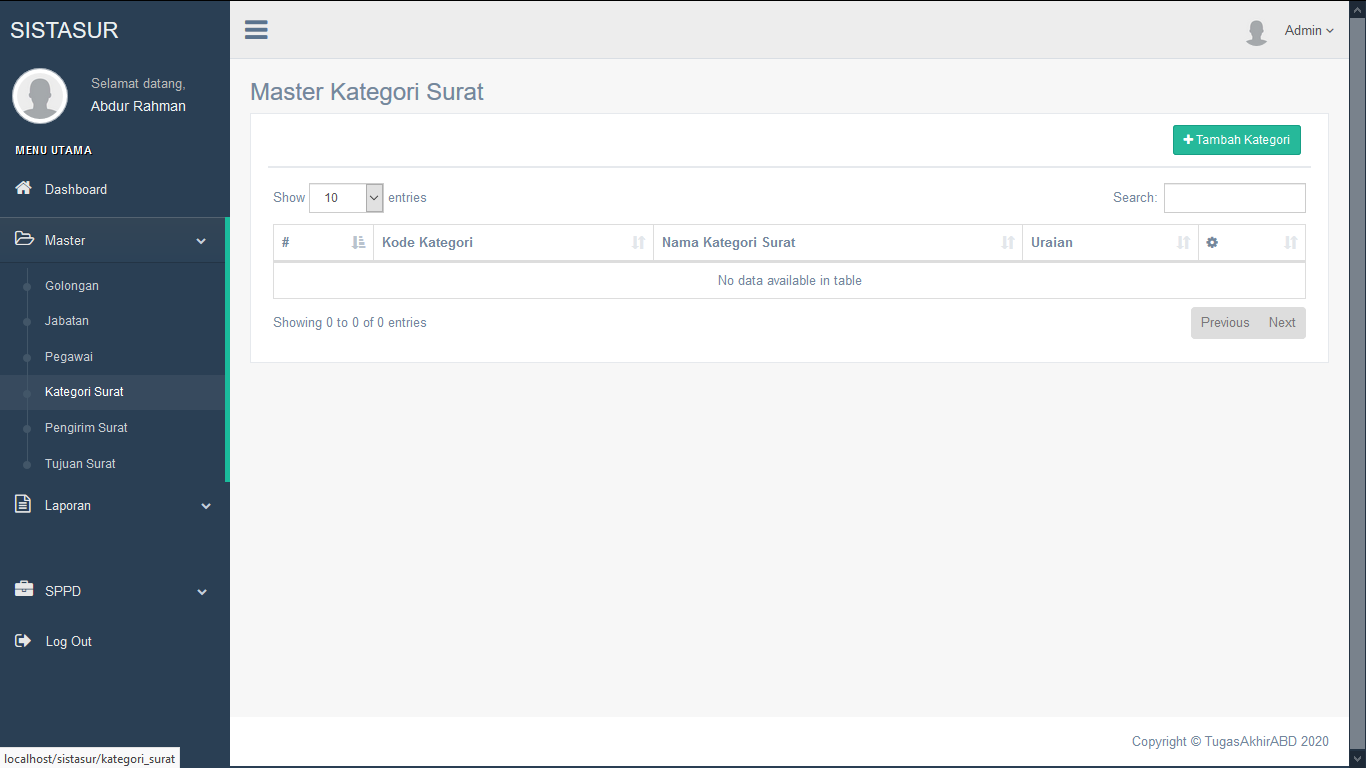
\includegraphics [height= 7cm, width=11cm]{konten/gambar/UISistemSurat/Admin/8.LihatKategoriSurat.png}
			\caption{Lihat Kategori Surat}
			\label{LihatKategoriSurat}
		\end{figure}
		
		\item Tambah Kategori Surat
		
		Berikut adalah tampilan Menambah Kategori Surat dapat dilihat pada \pic~\ref{TambahKategoriSurat}
		
		\begin{figure}
			\centering
			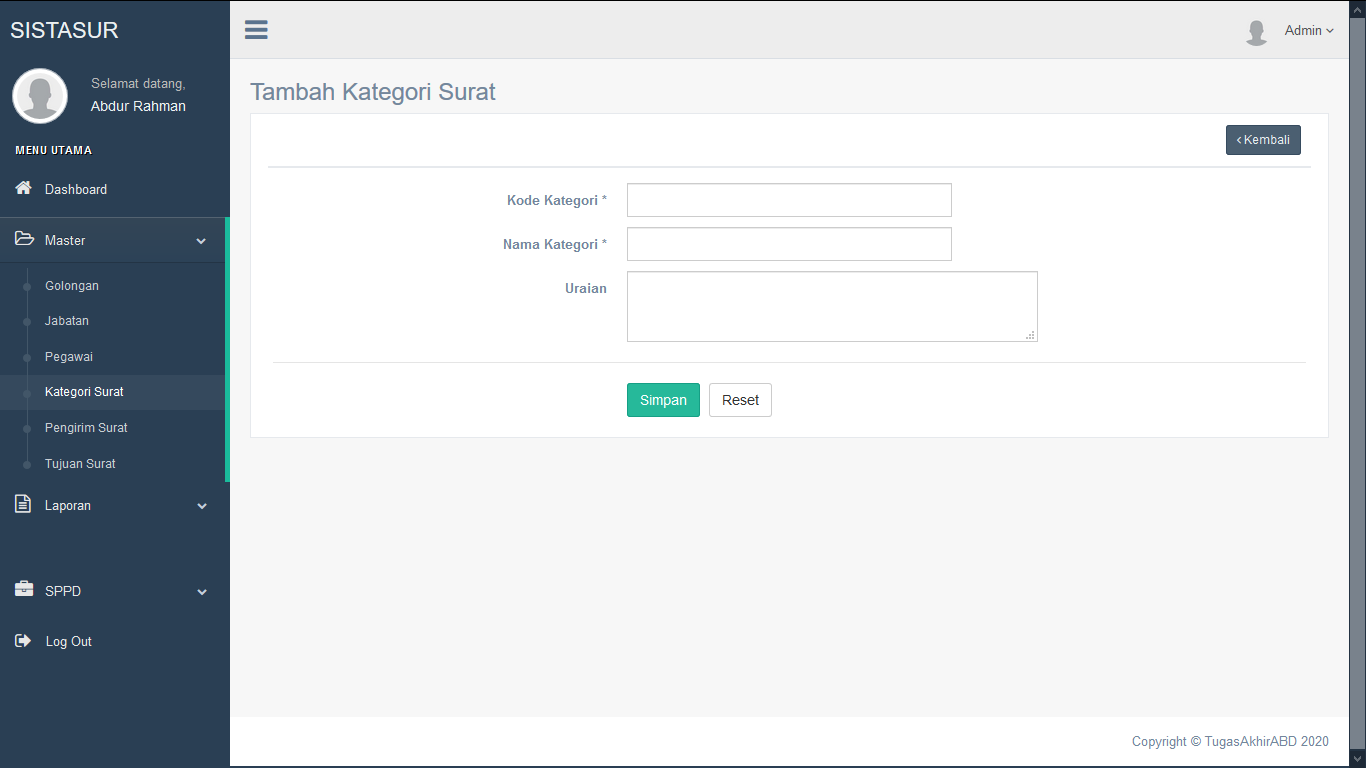
\includegraphics [height= 7cm, width=11cm]{konten/gambar/UISistemSurat/Admin/9.TambahKategoriSurat.png}
			\caption{Tambah Kategori Surat}
			\label{TambahKategoriSurat}
		\end{figure}
		
		\item Lihat Master Pengirim Surat
		
		Berikut adalah tampilan Melihat Master Pengirim Surat dapat dilihat pada \pic~\ref{LihatMasterPengirimSurat}
		
		\begin{figure}
			\centering
			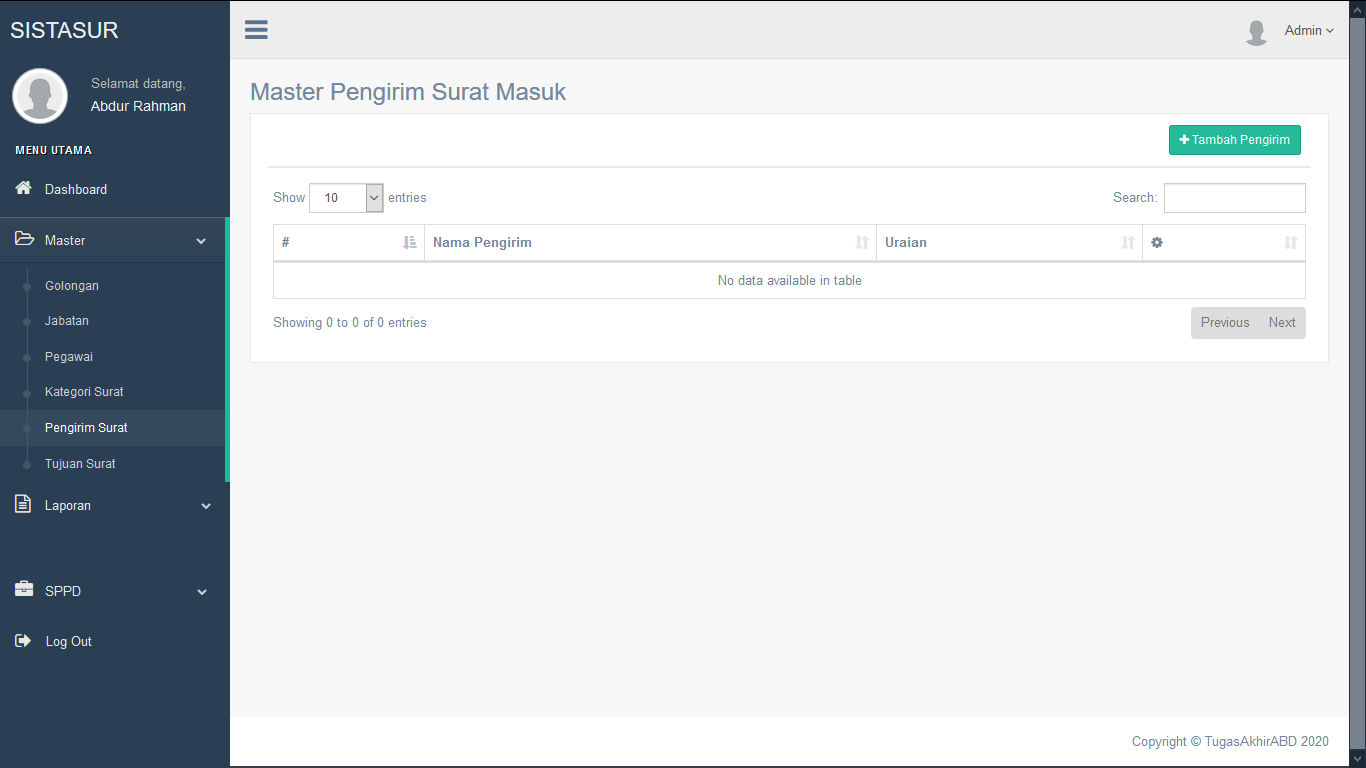
\includegraphics [height= 7cm, width=11cm]{konten/gambar/UISistemSurat/Admin/10.LihatMasterPengirimSurat.png}
			\caption{Lihat Master Pengirim Surat}
			\label{LihatMasterPengirimSurat}
		\end{figure}
		
		\item Tambah Data Pengirim Surat
		
		Berikut adalah tampilan Tambah Data Pengirim Surat dapat dilihat pada \pic~\ref{TambahDataPengirimSurat}
		
		\begin{figure}
			\centering
			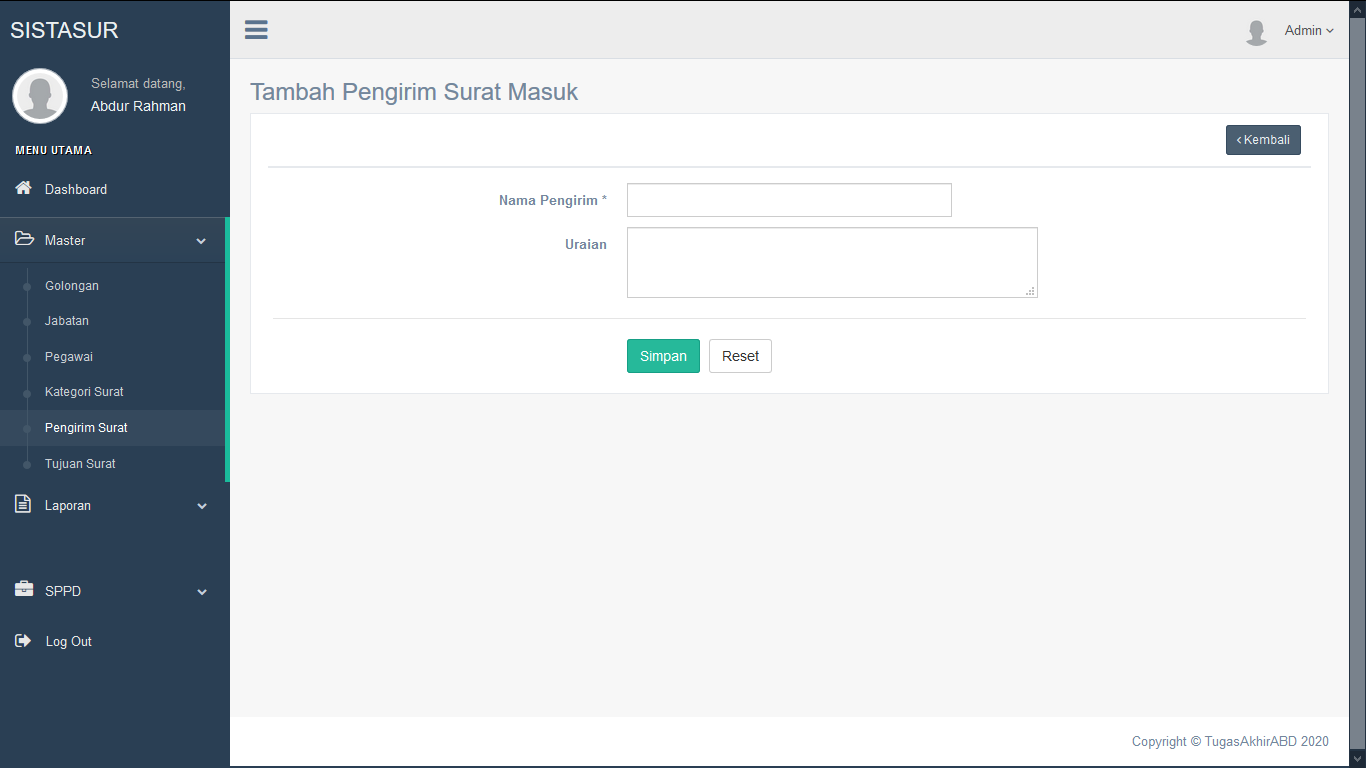
\includegraphics [height= 7cm, width=11cm]{konten/gambar/UISistemSurat/Admin/11.TambahDataPengirimSurat.png}
			\caption{Tambah Data Pengirim Surat}
			\label{TambahDataPengirimSurat}
		\end{figure}
		
		\item Lihat Tujuan Surat Keluar
		
		Berikut adalah tampilan Lihat Tujuan Surat Keluar dapat dilihat pada \pic~\ref{LihatTujuanSuratKeluar}
		
		\begin{figure}
			\centering
			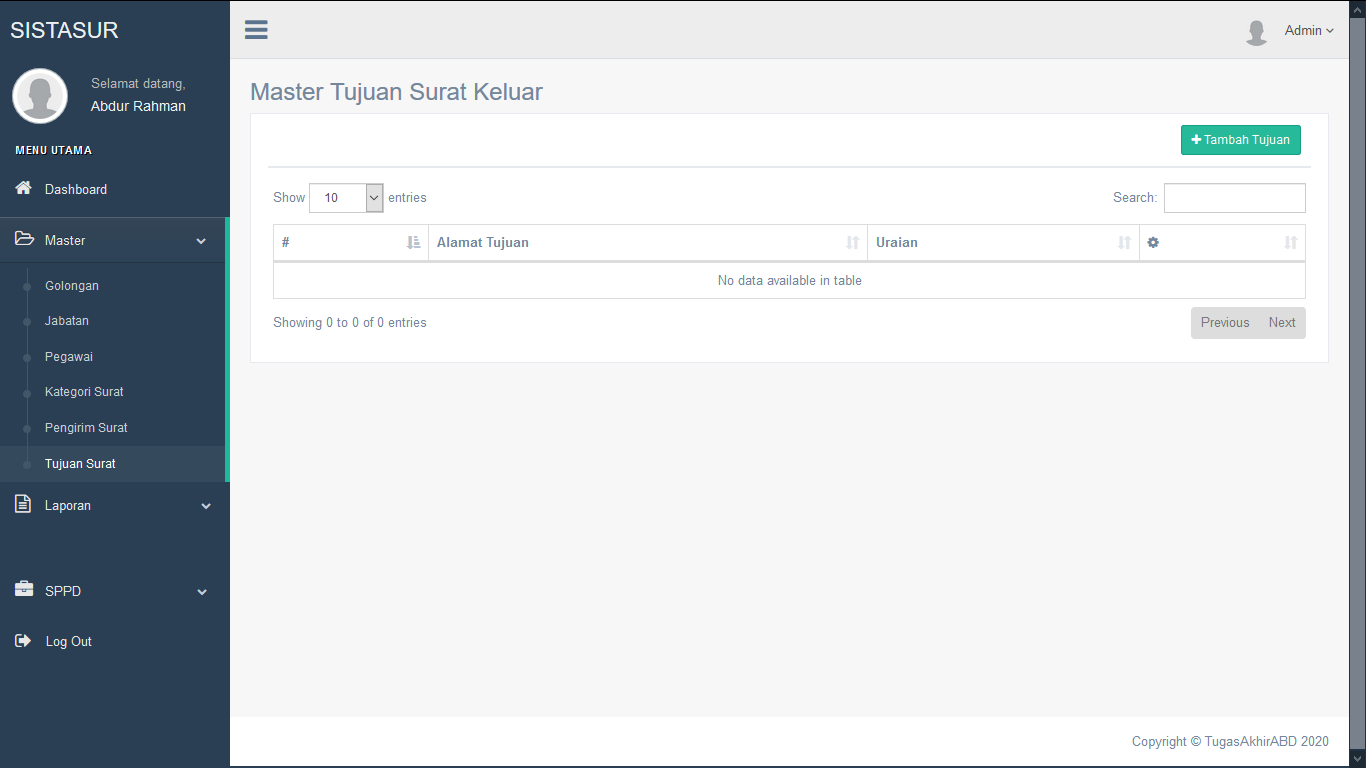
\includegraphics [height= 7cm, width=11cm]{konten/gambar/UISistemSurat/Admin/12.LihatTujuanSuratKeluar.png}
			\caption{Lihat Tujuan Surat Keluar}
			\label{LihatTujuanSuratKeluar}
		\end{figure}
		
		\item Tambah Data Tujuan Surat Keluar
		
		Berikut adalah tampilan Tambah Data Tujuan Surat Keluar dapat dilihat pada \pic~\ref{TambahDataTujuanSuratKeluar}
		
		\begin{figure}
			\centering
			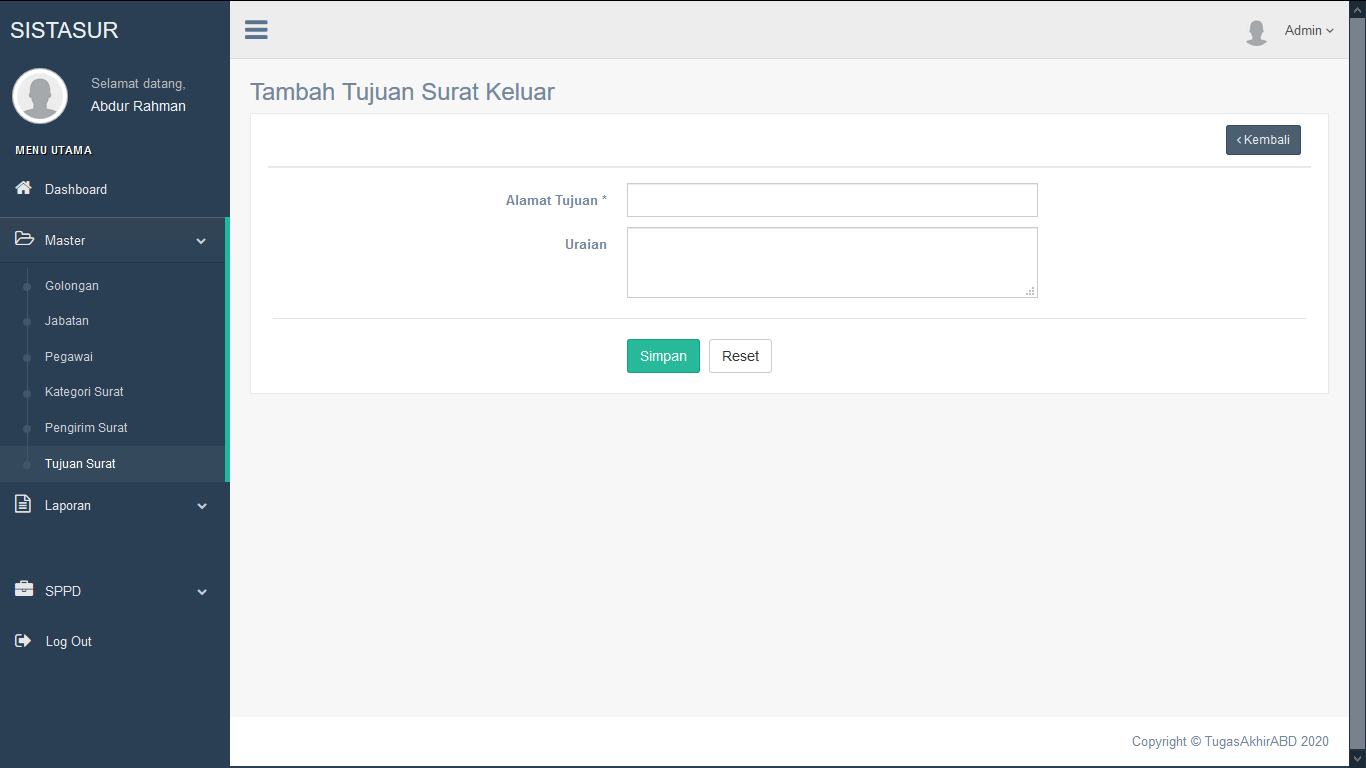
\includegraphics [height= 7cm, width=11cm]{konten/gambar/UISistemSurat/Admin/13.TambahDataTujuanSuratKeluar.png}
			\caption{Tambah Data Tujuan Surat Keluar}
			\label{TambahDataTujuanSuratKeluar}
		\end{figure}
		
		\item Lihat Data Surat Masuk
		
		Berikut adalah tampilan Lihat Data Surat Masuk dapat dilihat pada \pic~\ref{LihatDataSuratMasuk}
		
		\begin{figure}
			\centering
			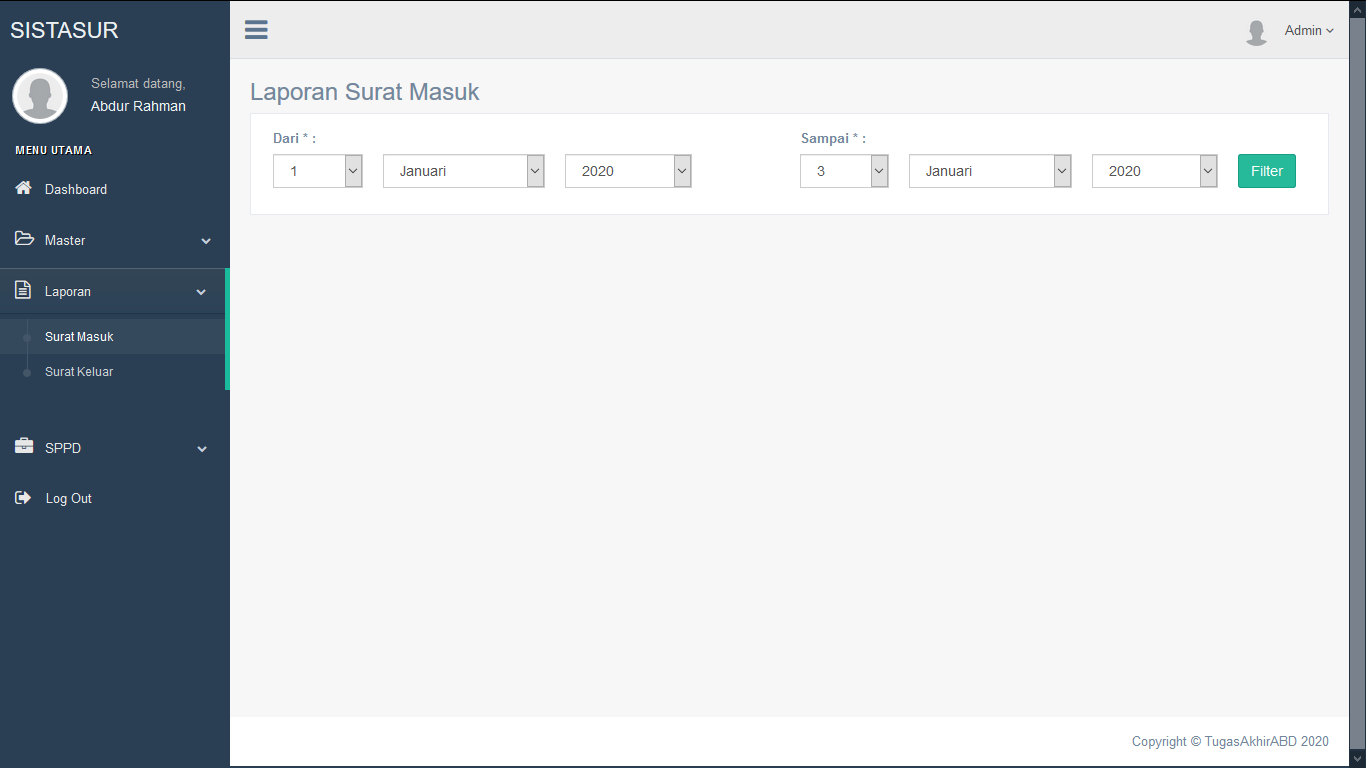
\includegraphics [height= 7cm, width=11cm]{konten/gambar/UISistemSurat/Admin/14.LihatDataSuratMasuk.png}
			\caption{Lihat Data Surat Masuk}
			\label{LihatDataSuratMasuk}
		\end{figure}
		
		\item Lihat Data Surat Keluar
		
		Berikut adalah tampilan Lihat Data Surat Keluar dapat dilihat pada \pic~\ref{LihatDataSuratKeluar}
		
		\begin{figure}
			\centering
			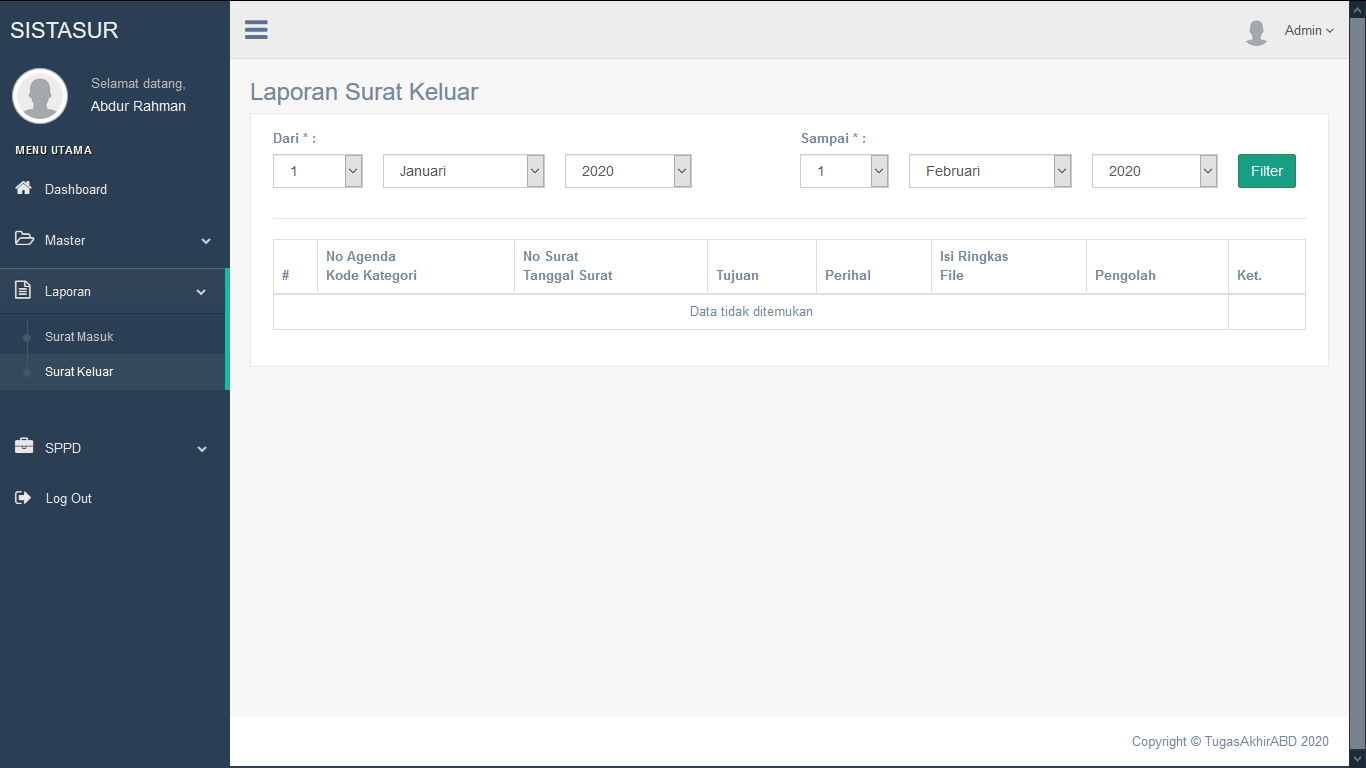
\includegraphics [height= 7cm, width=11cm]{konten/gambar/UISistemSurat/Admin/15.LihatDataSuratKeluar.png}
			\caption{Lihat Data Surat Keluar}
			\label{LihatDataSuratKeluar}
		\end{figure}
		
		\item Tambah Data SPPD
		
		Berikut adalah tampilan Tambah Data SPPD dapat dilihat pada \pic~\ref{TambahDataSPPDAdmin}
		
		\begin{figure}
			\centering
			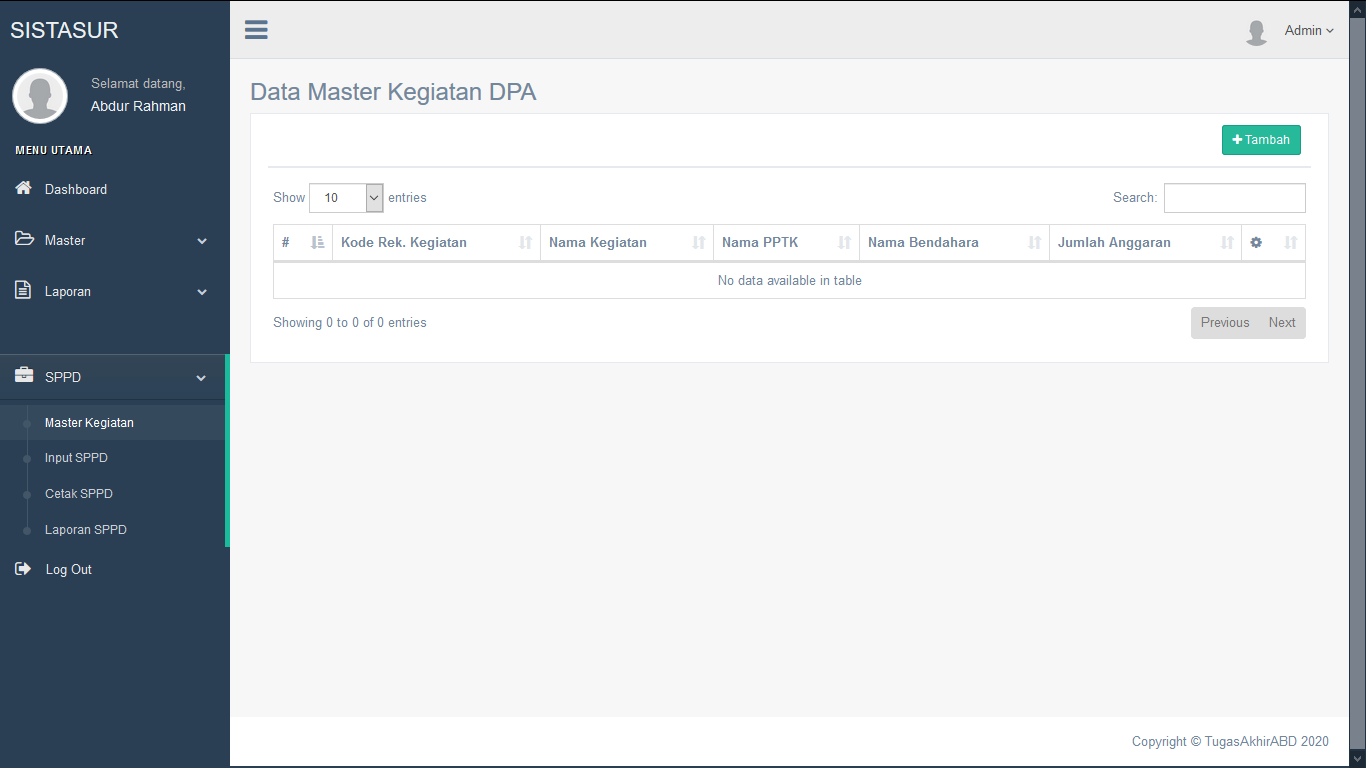
\includegraphics [height= 7cm, width=11cm]{konten/gambar/UISistemSurat/Admin/16.TambahDataSPPD.png}
			\caption{Tambah Data SPPD}
			\label{TambahDataSPPDAdmin}
		\end{figure}
		
		\item Tambah Data SPPD Master
		
		Berikut adalah tampilan Tambah Data SPPD Master dapat dilihat pada \pic~\ref{TambahDataSPPDMasterAdmin}
		
		\begin{figure}
			\centering
			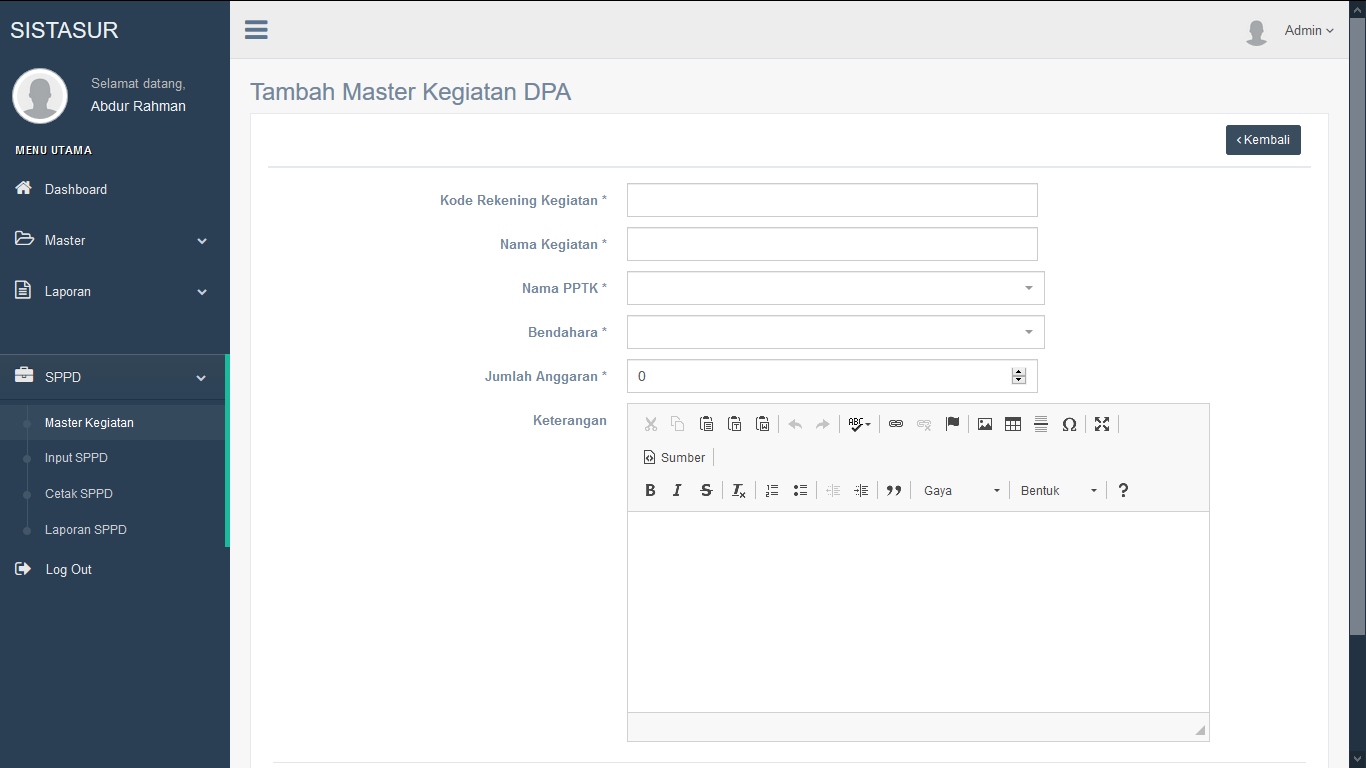
\includegraphics [height= 7cm, width=11cm]{konten/gambar/UISistemSurat/Admin/17.TambahDataSPPDMaster.png}
			\caption{Tambah Data SPPD Master}
			\label{TambahDataSPPDMasterAdmin}
		\end{figure}
		
		\item Lihat Data SPPD
		
		Berikut adalah tampilan Lihat Data SPPD dapat dilihat pada \pic~\ref{LihatDataSPPDAdmin}
		
		\begin{figure}
			\centering
			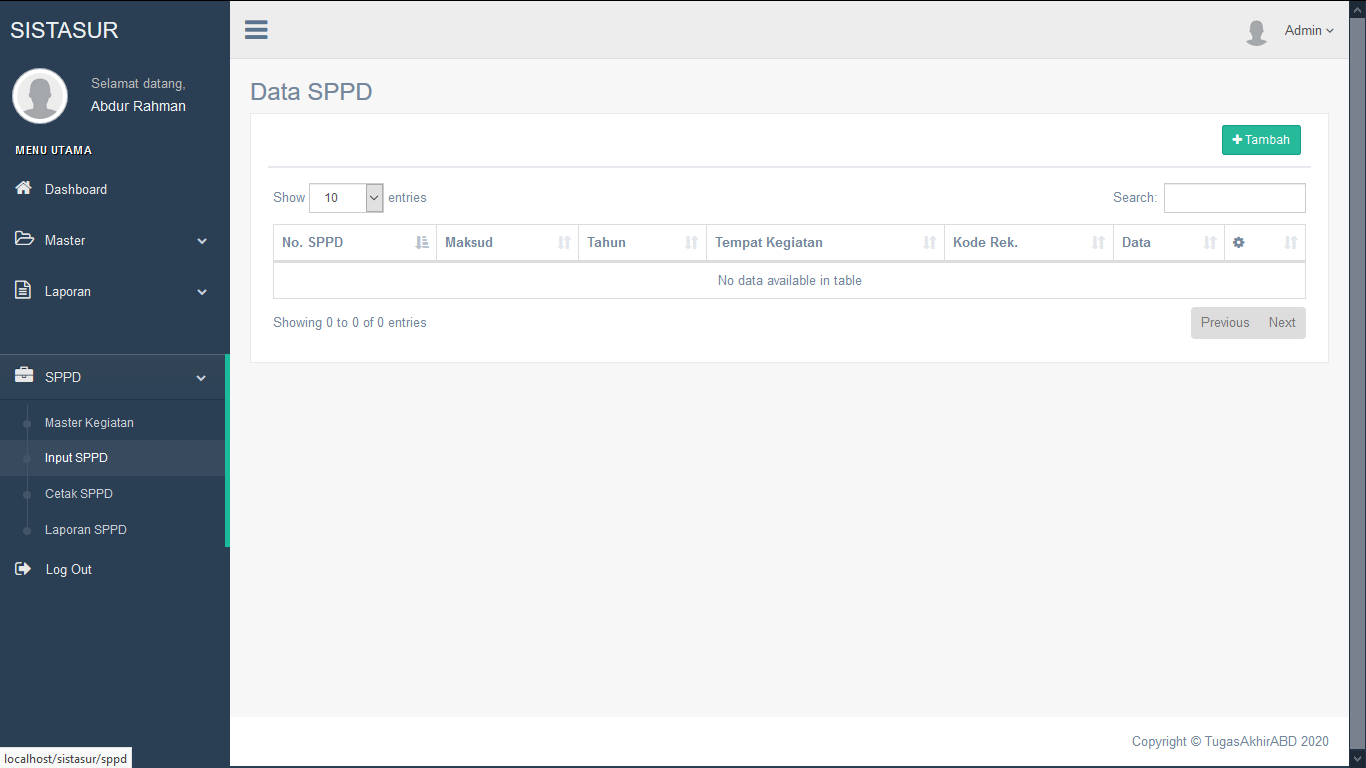
\includegraphics [height= 7cm, width=11cm]{konten/gambar/UISistemSurat/Admin/18.LihatDataSPPD.png}
			\caption{Lihat Data SPPD}
			\label{LihatDataSPPDAdmin}
		\end{figure}
		
		\item Cetak SPPD
		
		Berikut adalah tampilan Cetak SPPD dapat dilihat pada \pic~\ref{CetakSPPDAdmin}
		
		\begin{figure}
			\centering
			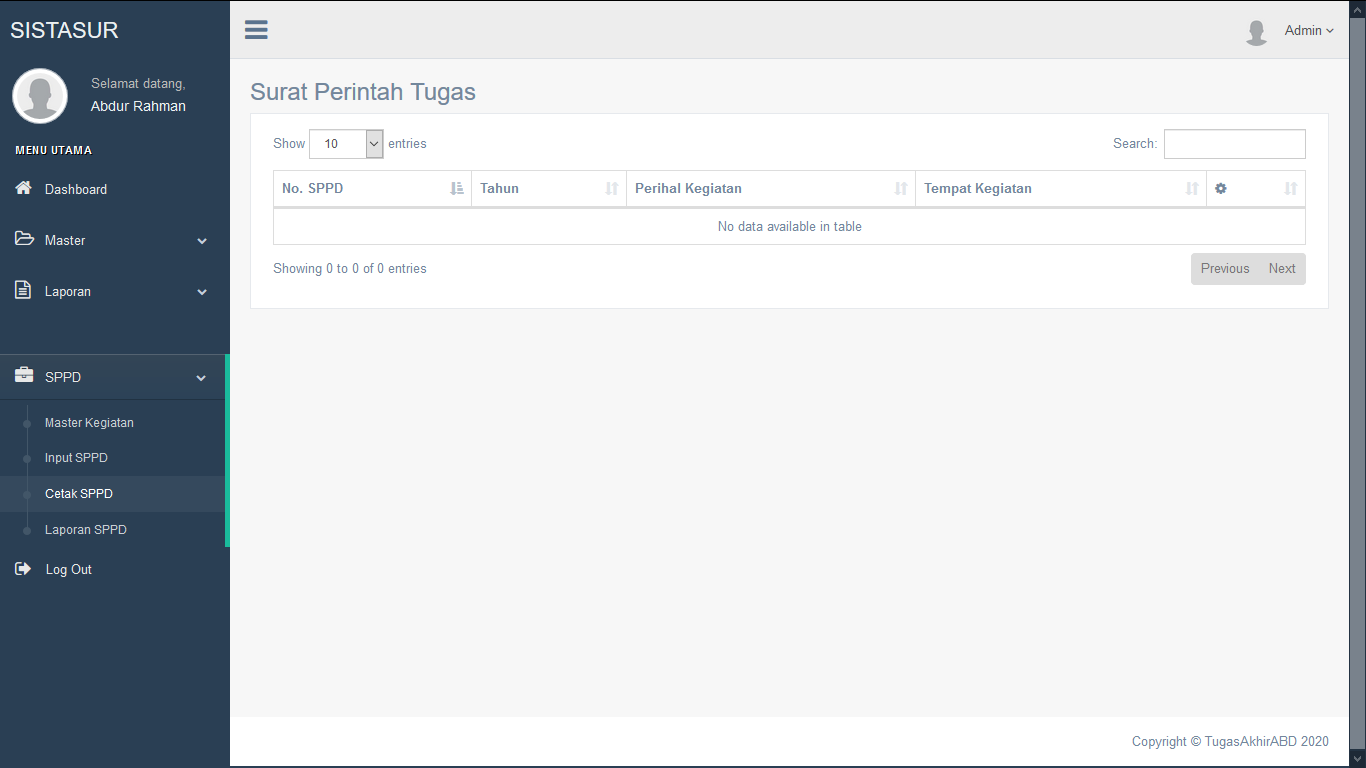
\includegraphics [height= 7cm, width=11cm]{konten/gambar/UISistemSurat/Admin/20.CetakSPPD.png}
			\caption{Cetak SPPD}
			\label{CetakSPPDAdmin}
		\end{figure}
		
		\item Rekap Data SPPD
		
		Berikut adalah tampilan Rekap Data SPPD dapat dilihat pada \pic~\ref{RekapDataSPPDAdmin}
		
		\begin{figure}
			\centering
			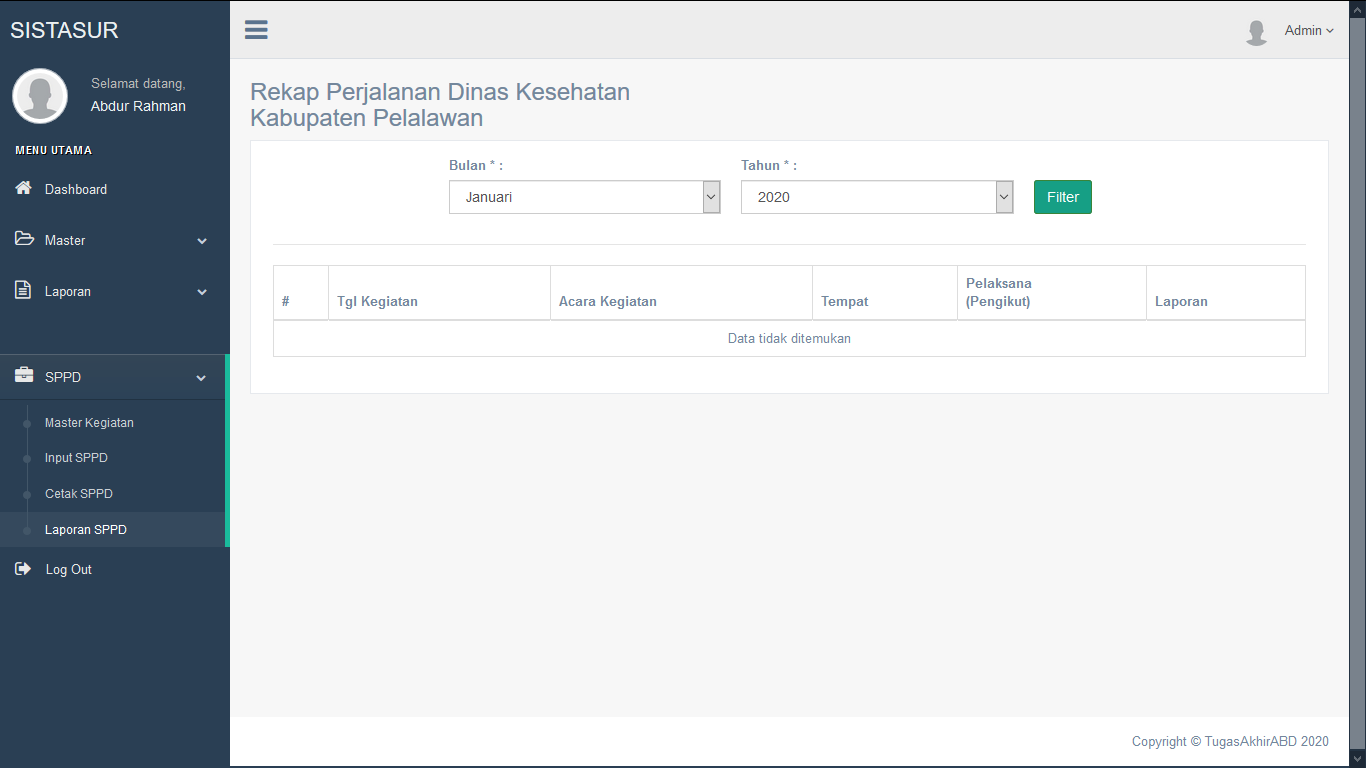
\includegraphics [height= 7cm, width=11cm]{konten/gambar/UISistemSurat/Admin/21.RekapDataSPPD.png}
			\caption{RekapDataSPPD}
			\label{RekapDataSPPDAdmin}
		\end{figure}	
	\end{enumerate}
	
	\item \textbf{Kepala Dinas}
	
	\begin{enumerate}
		\item Dashboard
		
		Berikut adalah tampilan Dashboard Kepala Dinas dapat dilihat pada \pic~\ref{DashboardKadis}
		
		\begin{figure}
			\centering
			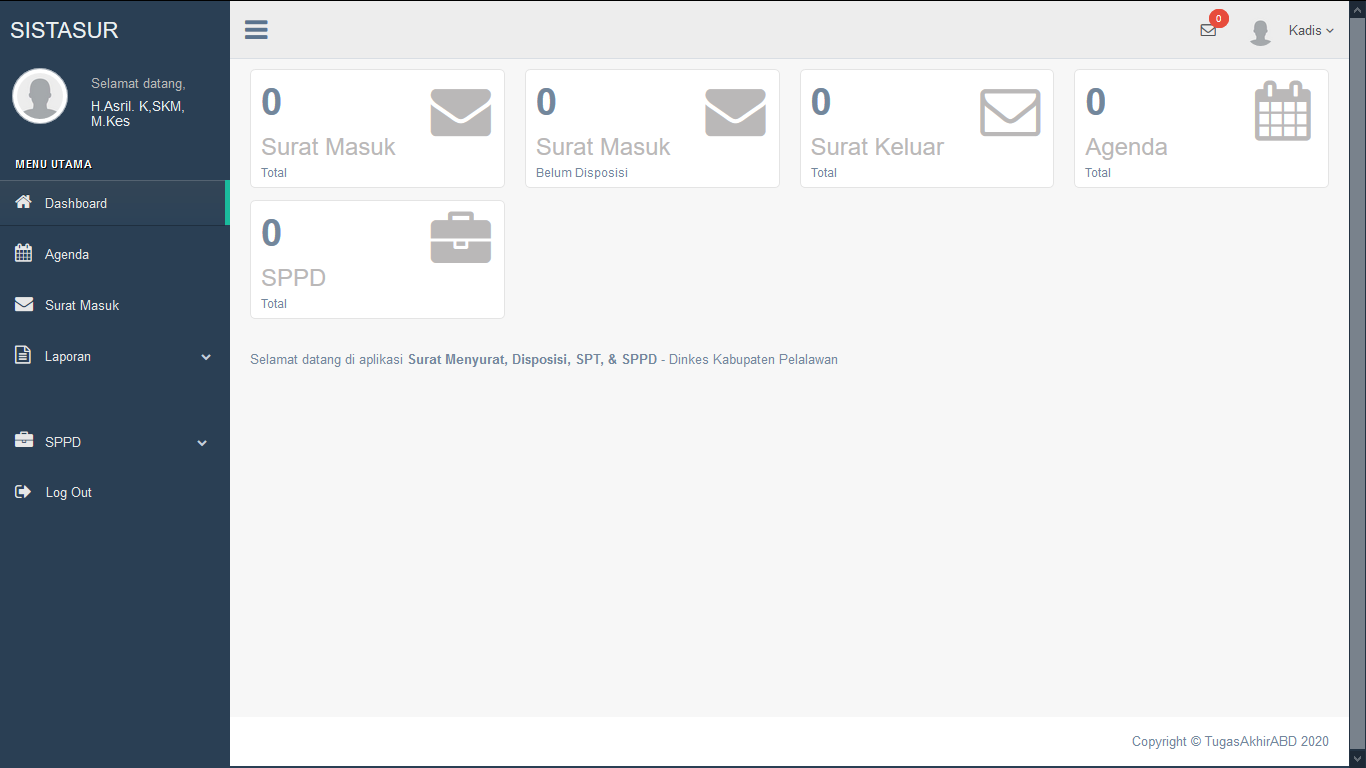
\includegraphics [height= 7cm, width=11cm]{konten/gambar/UISistemSurat/Kadis/0.1.Dashboard.png}
			\caption{Dashboard Kadis}
			\label{DashboardKadis}
		\end{figure}
		
		\item Notifikasi Disposisi
		
		Berikut adalah tampilan Notifikasi Disposisi dapat dilihat pada \pic~\ref{DashboardKadis}
		
		\begin{figure}
			\centering
			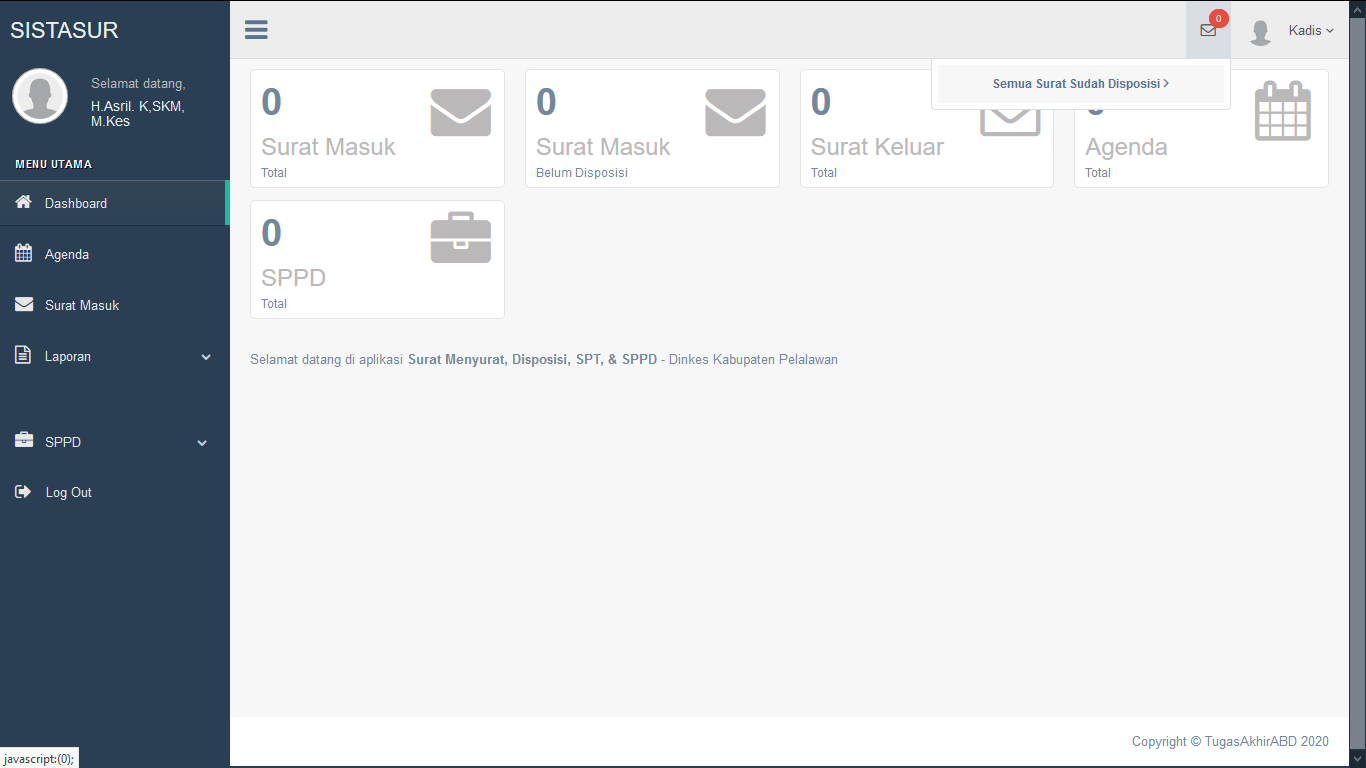
\includegraphics [height= 7cm, width=11cm]{konten/gambar/UISistemSurat/Kadis/0.2.notifikasiDisposisi.png}
			\caption{Notifikasi Disposisi}
			\label{notifikasiDisposisi}
		\end{figure}
		
		\item Halaman Profile
		
		Berikut adalah tampilan Halaman Profile Kadis dapat dilihat pada \pic~\ref{HalamanProfileKadis}
		
		\begin{figure}
			\centering
			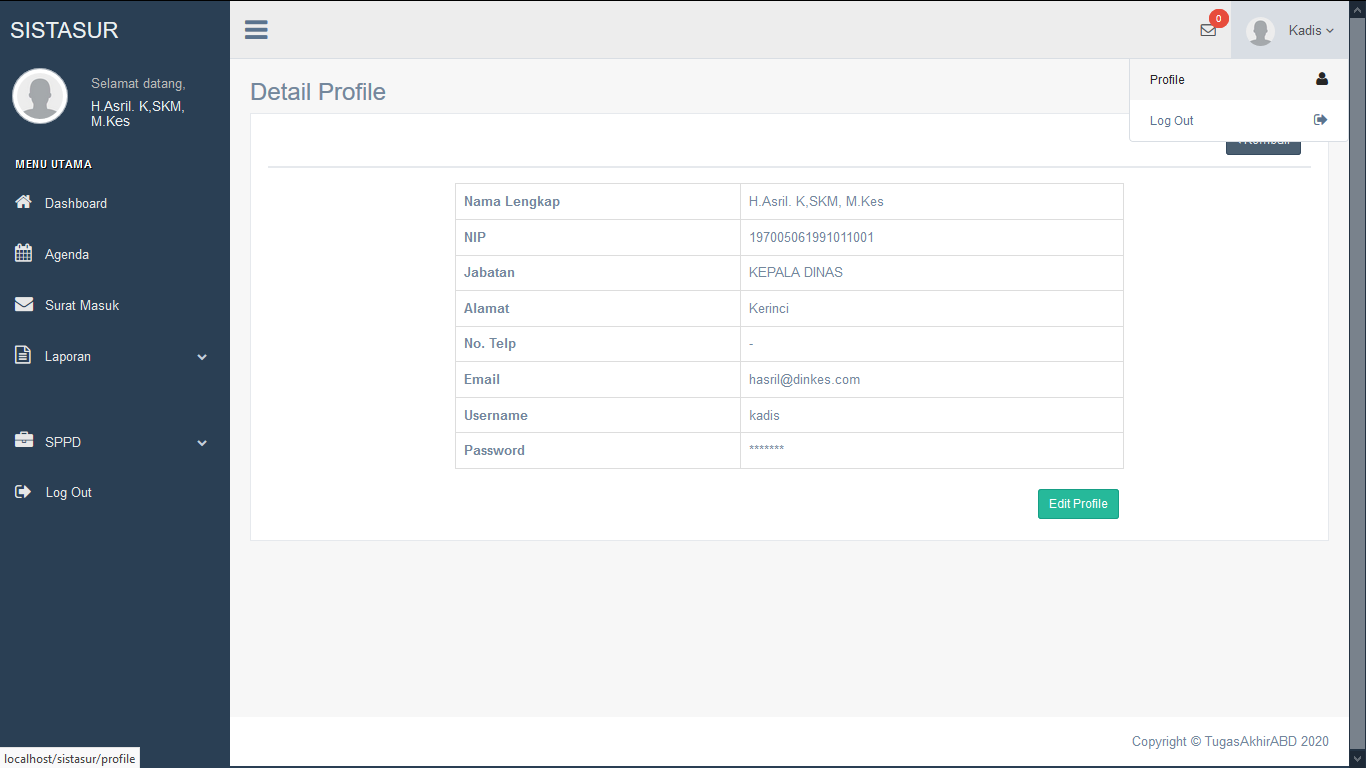
\includegraphics [height= 7cm, width=11cm]{konten/gambar/UISistemSurat/Kadis/0.3.HalamanProfile.png}
			\caption{Halaman Profile Kadis}
			\label{HalamanProfileKadis}
		\end{figure}
		
		\item Lihat Master Agenda
		
		Berikut adalah tampilan Lihat Master Agenda Kadis dapat dilihat pada \pic~\ref{LihatMasterAgendaKadis}
		
		\begin{figure}
			\centering
			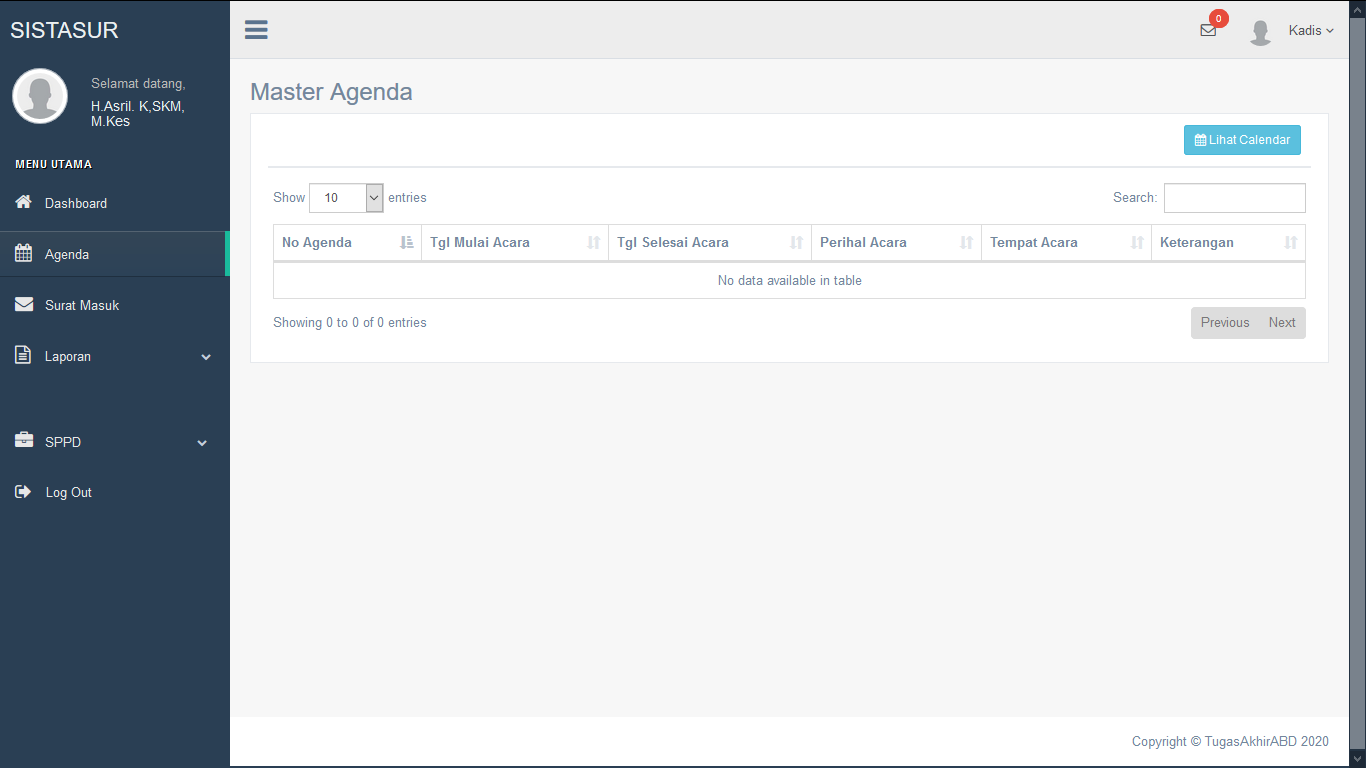
\includegraphics [height= 7cm, width=11cm]{konten/gambar/UISistemSurat/Kadis/0.4.LihatMasterAgenda.png}
			\caption{Lihat Master Agenda Kadis}
			\label{LihatMasterAgendaKadis}
		\end{figure}
		
		\item Lihat Master Agenda Bulanan
		
		Berikut adalah tampilan Lihat Master Agenda Bulanan Kadis dapat dilihat pada \pic~\ref{LihatMasterAgendaBulananKadis}
		
		\begin{figure}
			\centering
			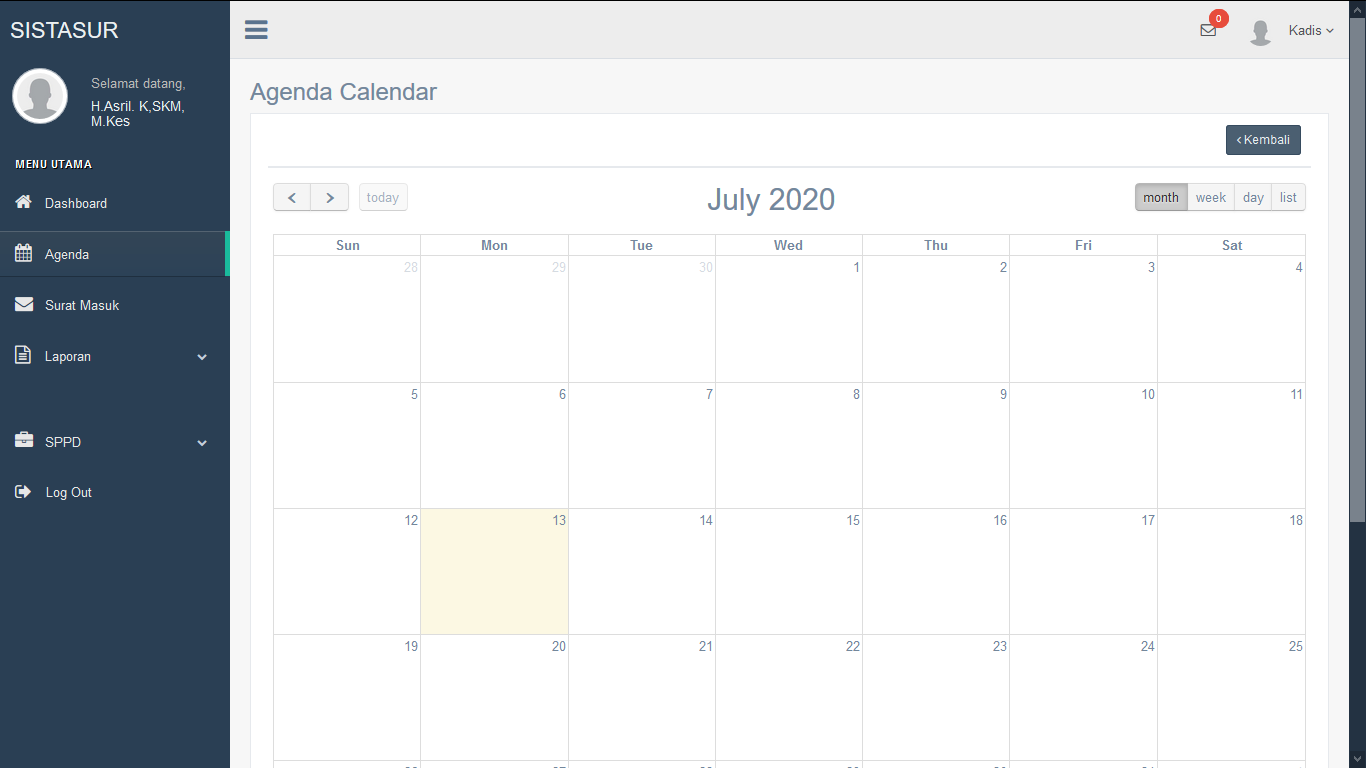
\includegraphics [height= 7cm, width=11cm]{konten/gambar/UISistemSurat/Kadis/0.5.LihatMasterAgendaBulanan.png}
			\caption{Lihat Master Agenda Bulanan Kadis}
			\label{LihatMasterAgendaBulananKadis}
		\end{figure}
		
		\item Lihat Master Agenda Mingguan
		
		Berikut adalah tampilan Lihat Master Agenda Mingguan Kadis dapat dilihat pada \pic~\ref{LihatMasterAgendaMingguanKadis}
		
		\begin{figure}
			\centering
			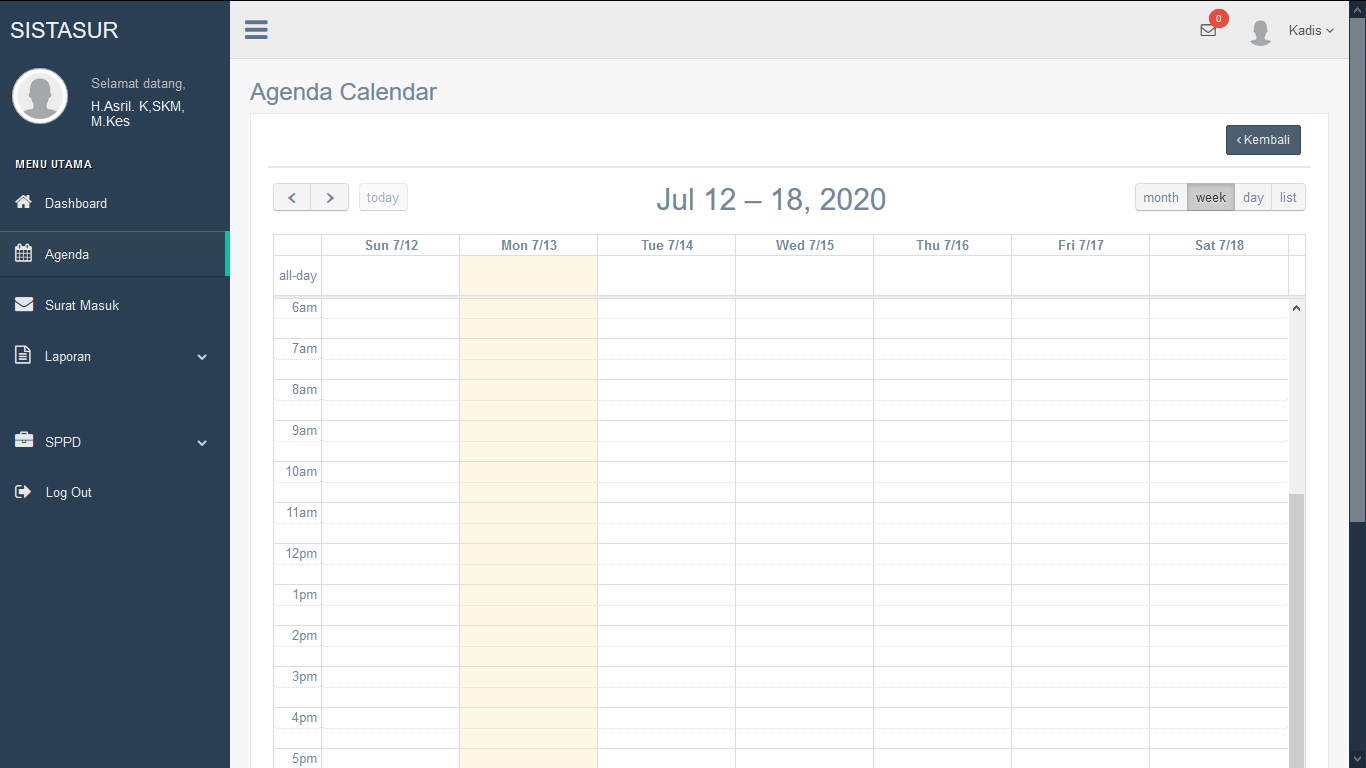
\includegraphics [height= 7cm, width=11cm]{konten/gambar/UISistemSurat/Kadis/0.6.LihatMasterAgendaMingguan.png}
			\caption{Lihat Master Agenda Mingguan Kadis}
			\label{LihatMasterAgendaMingguanKadis}
		\end{figure}
		
		\item Lihat Master Agenda Harian
		
		Berikut adalah tampilan Lihat Master Agenda Harian Kadis dapat dilihat pada \pic~\ref{LihatMasterAgendaHarianKadis}
		
		\begin{figure}
			\centering
			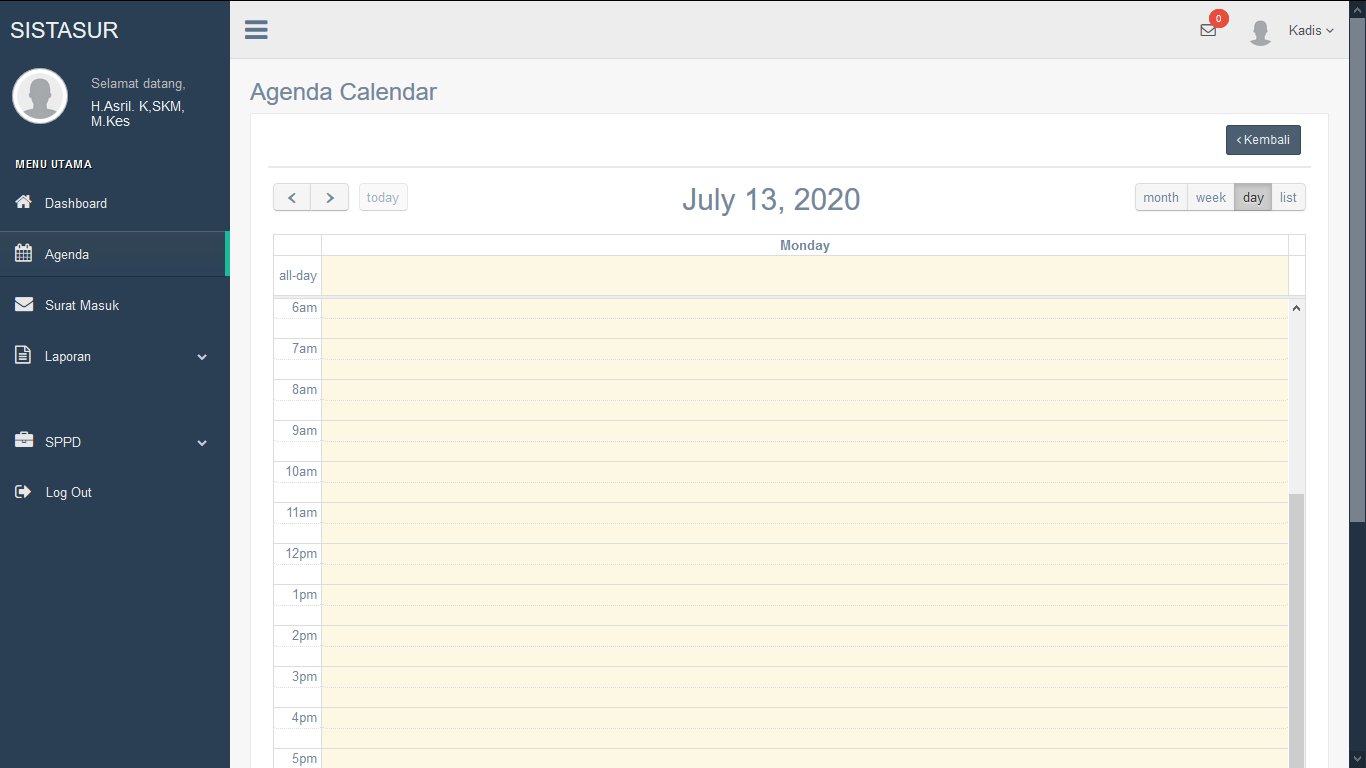
\includegraphics [height= 7cm, width=11cm]{konten/gambar/UISistemSurat/Kadis/0.7.LihatMasterAgendaHarian.png}
			\caption{Lihat Master Agenda Harian Kadis}
			\label{LihatMasterAgendaHarianKadis}
		\end{figure}
		
		\item Lihat Data Surat Masuk
		
		Berikut adalah tampilan Lihat Data Surat Masuk Kadis dapat dilihat pada \pic~\ref{LihatDataSuratMasukKadis}
		
		\begin{figure}
			\centering
			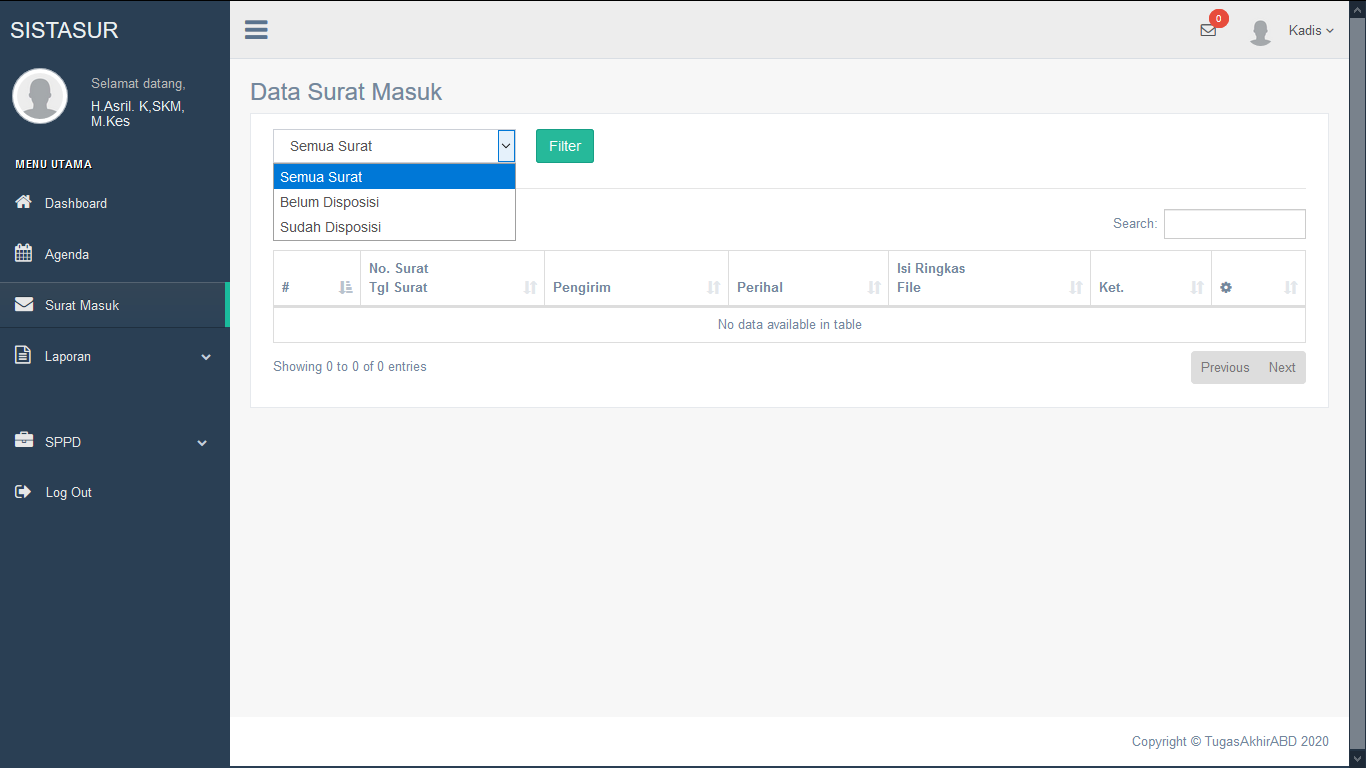
\includegraphics [height= 7cm, width=11cm]{konten/gambar/UISistemSurat/Kadis/0.8.LihatDataSuratMasuk.png}
			\caption{Lihat Data Surat Masuk Kadis}
			\label{LihatDataSuratMasukKadis}
		\end{figure}
		
		\item Lihat Laporan Surat Masuk
		
		Berikut adalah tampilan Lihat Laporan Surat Masuk Kadis dapat dilihat pada \pic~\ref{LihatLaporanSuratMasukKadis}
		
		\begin{figure}
			\centering
			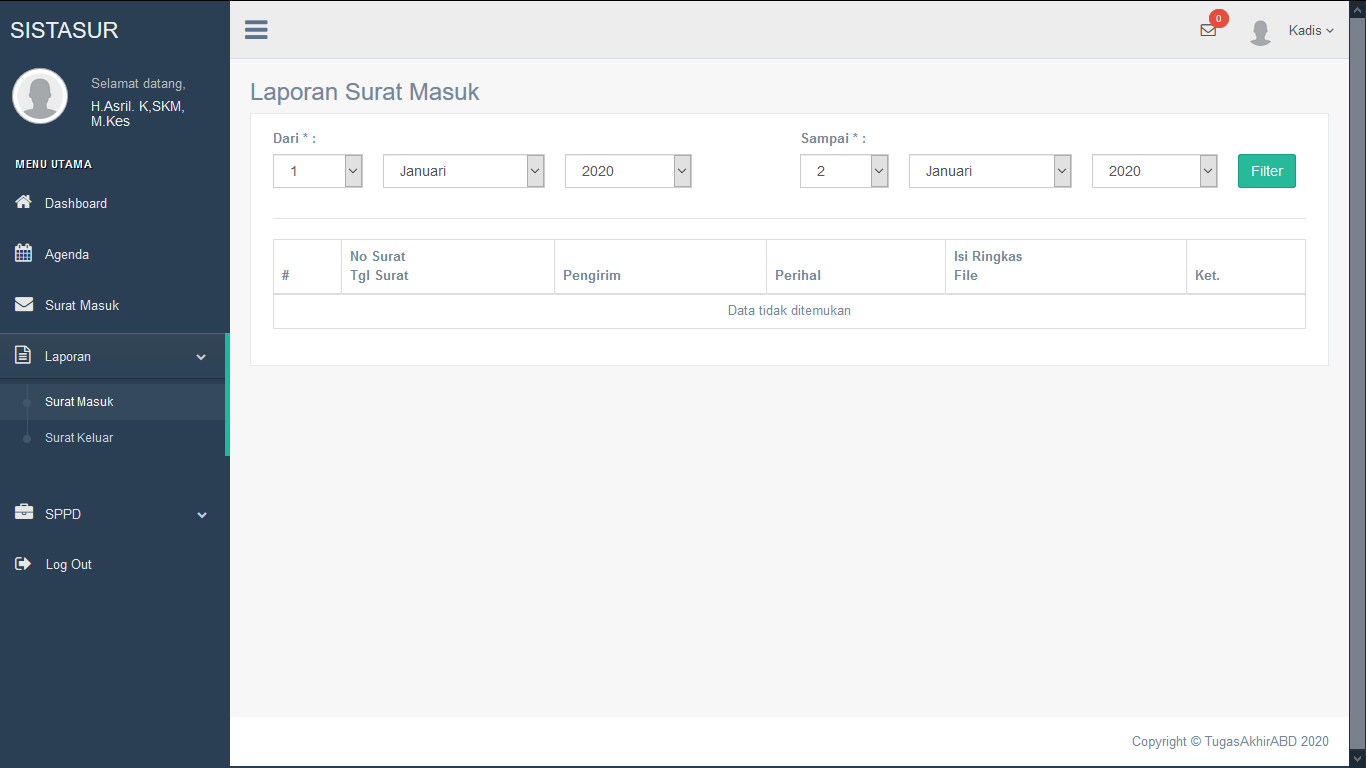
\includegraphics [height= 7cm, width=11cm]{konten/gambar/UISistemSurat/Kadis/0.9.LihatLaporanSuratMasuk.png}
			\caption{Lihat Laporan Surat Masuk Kadis}
			\label{LihatLaporanSuratMasukKadis}
		\end{figure}
		
		\item Lihat Laporan Surat Keluar
		
		Berikut adalah tampilan Lihat Laporan Surat Keluar Kadis dapat dilihat pada \pic~\ref{LihatLaporanSuratKeluarKadis}
		
		\begin{figure}
			\centering
			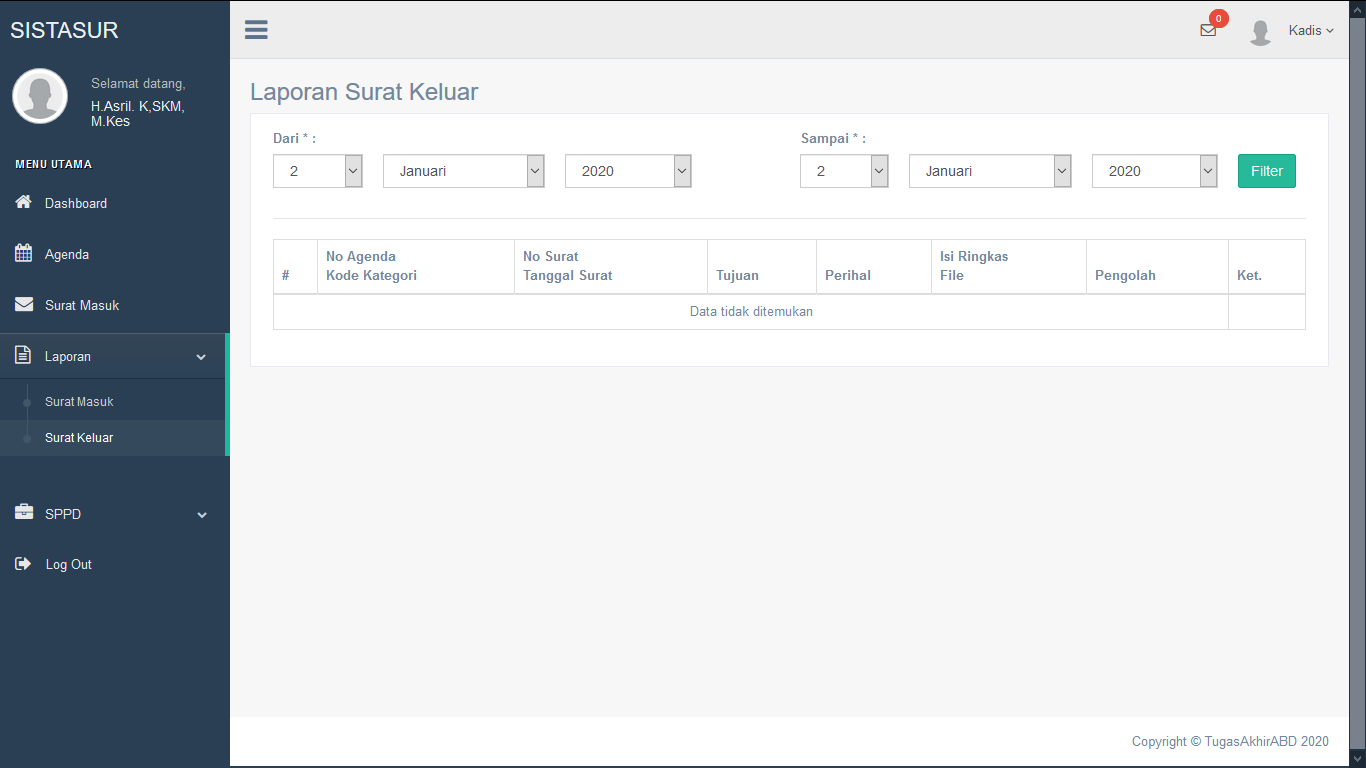
\includegraphics [height= 7cm, width=11cm]{konten/gambar/UISistemSurat/Kadis/0.10.LihatLaporanSuratKeluar.png}
			\caption{Lihat Laporan Surat Keluar Kadis}
			\label{LihatLaporanSuratKeluarKadis}
		\end{figure}
		
		\item Master Data Kegiatan
		
		Berikut adalah tampilan Master Data Kegiatan DPA Kadis dapat dilihat pada \pic~\ref{MasterDataKegiatanDPAKadis}
		
		\begin{figure}
			\centering
			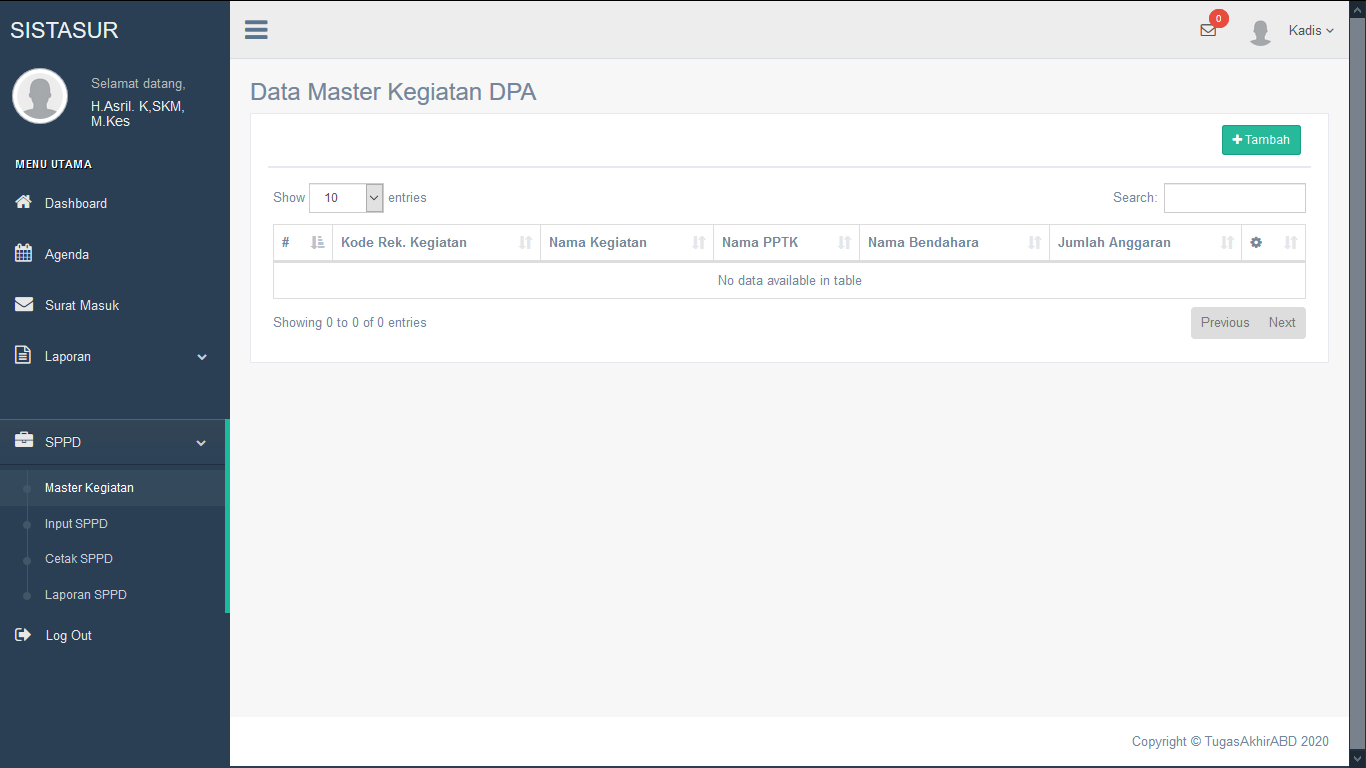
\includegraphics [height= 7cm, width=11cm]{konten/gambar/UISistemSurat/Kadis/0.11.MasterDataKegiatanDPA.png}
			\caption{Master Data Kegiatan DPA Kadis}
			\label{MasterDataKegiatanDPAKadis}
		\end{figure}
		
		\item Lihat Data Master
		
		Berikut adalah tampilan Lihat Data Master DPA Kadis dapat dilihat pada \pic~\ref{LihatDataMasterDPAKadis}
		
		\begin{figure}
			\centering
			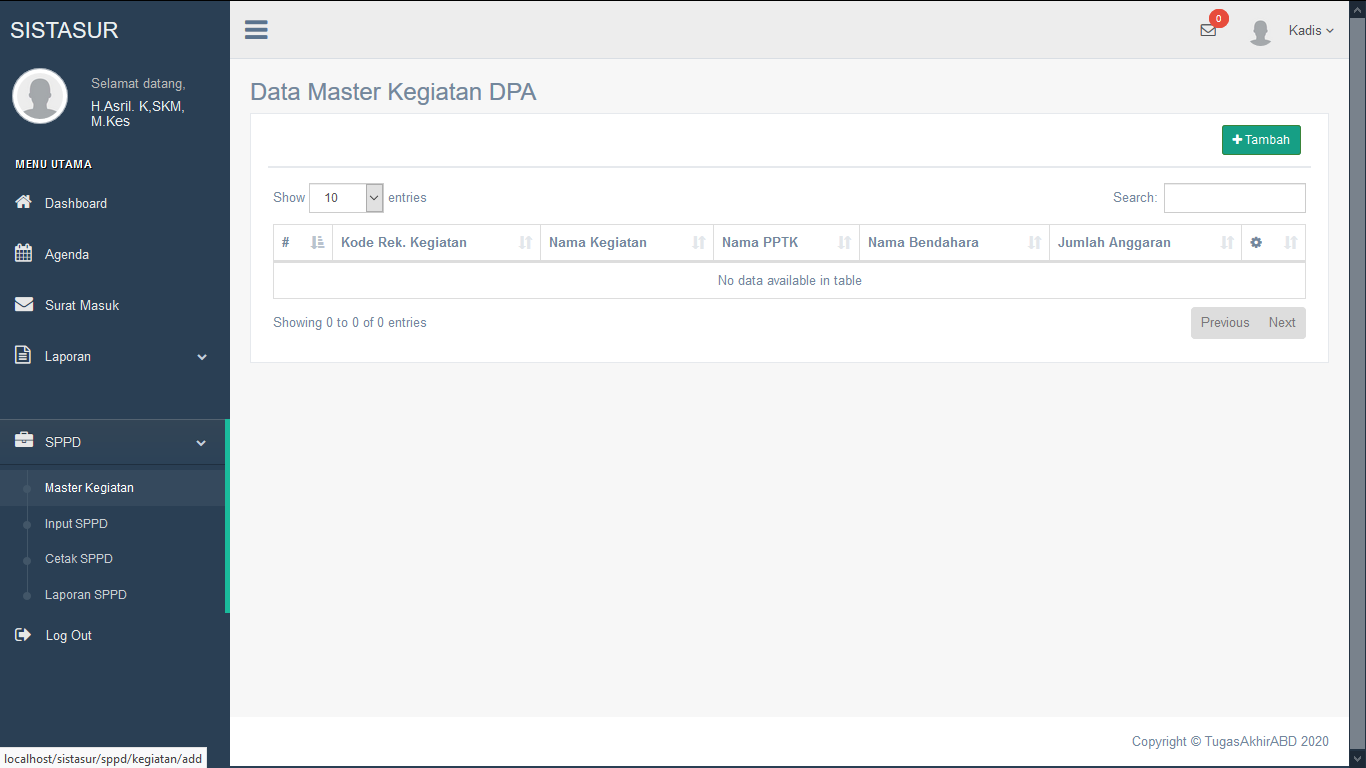
\includegraphics [height= 7cm, width=11cm]{konten/gambar/UISistemSurat/Kadis/0.12.LihatDataMasterDPA.png}
			\caption{Lihat Data Master DPA Kadis}
			\label{LihatDataMasterDPAKadis}
		\end{figure}
		
		\item Tambah Master Kegiatan
		
		Berikut adalah tampilan Tambah Master Kegiatan DPA Kadis dapat dilihat pada \pic~\ref{TambahMasterKegiatanDPAKadis}
		
		\begin{figure}
			\centering
			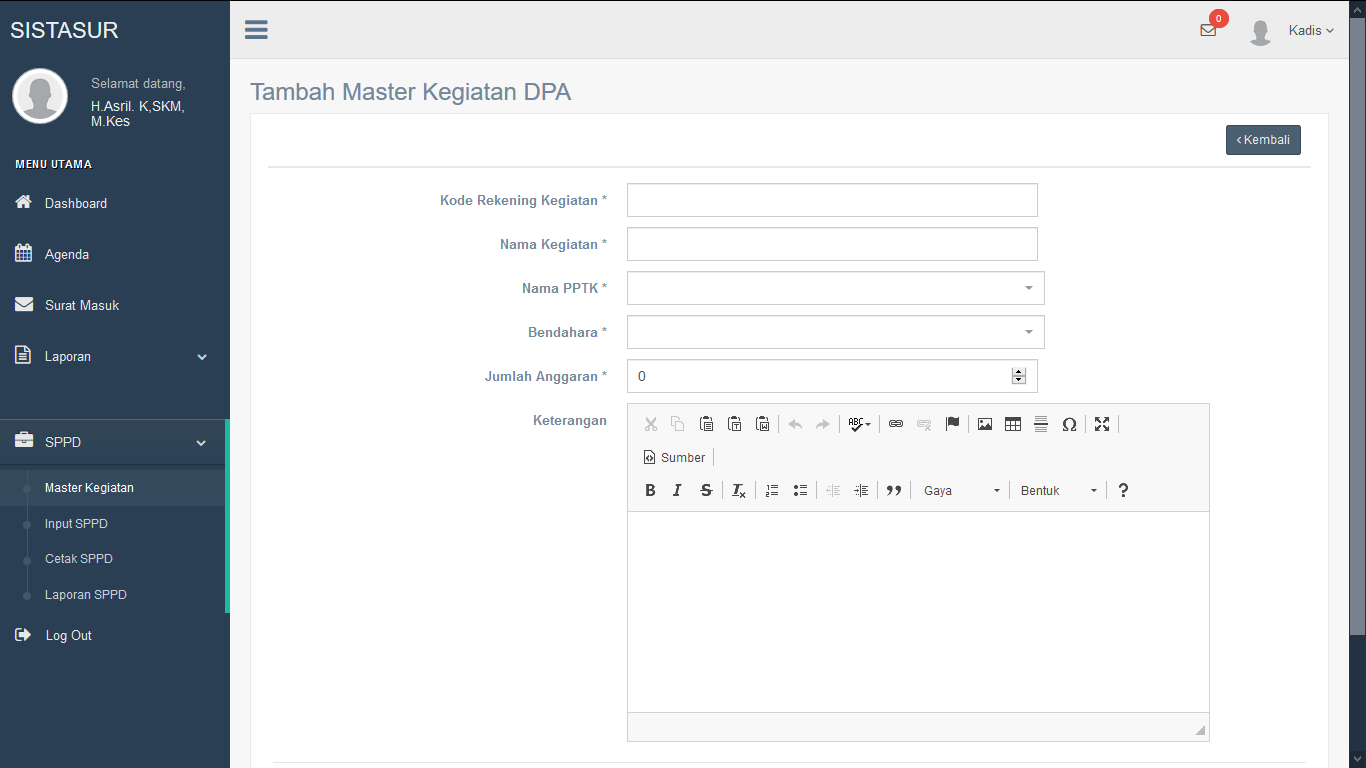
\includegraphics [height= 7cm, width=11cm]{konten/gambar/UISistemSurat/Kadis/0.13.TambahMasterKegiatanDPA.png}
			\caption{Tambah Master Kegiatan DPA Kadis}
			\label{TambahMasterKegiatanDPAKadis}
		\end{figure}
		
		\item Lihat Data SPPD
		
		Berikut adalah tampilan Lihat Data SPPD Kadis dapat dilihat pada \pic~\ref{LihatDataSPPDKadis}
		
		\begin{figure}
			\centering
			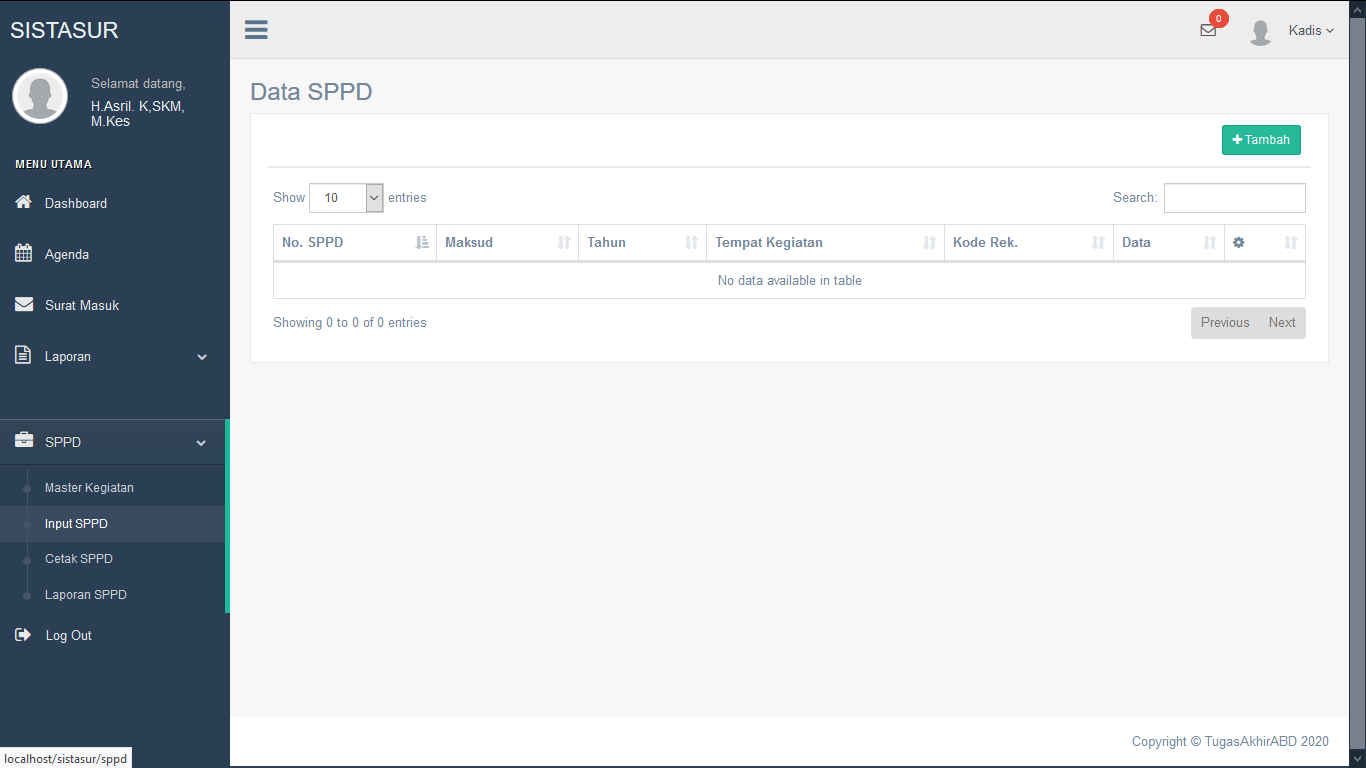
\includegraphics [height= 7cm, width=11cm]{konten/gambar/UISistemSurat/Kadis/0.14.LihatDataSPPD.png}
			\caption{Lihat Data SPPD Kadis}
			\label{LihatDataSPPDKadis}
		\end{figure}
		
		\item Input Data SPPD
		
		Berikut adalah tampilan Input Data SPPD Kadis dapat dilihat pada \pic~\ref{InputDataSPPDKadis}
		
		\begin{figure}
			\centering
			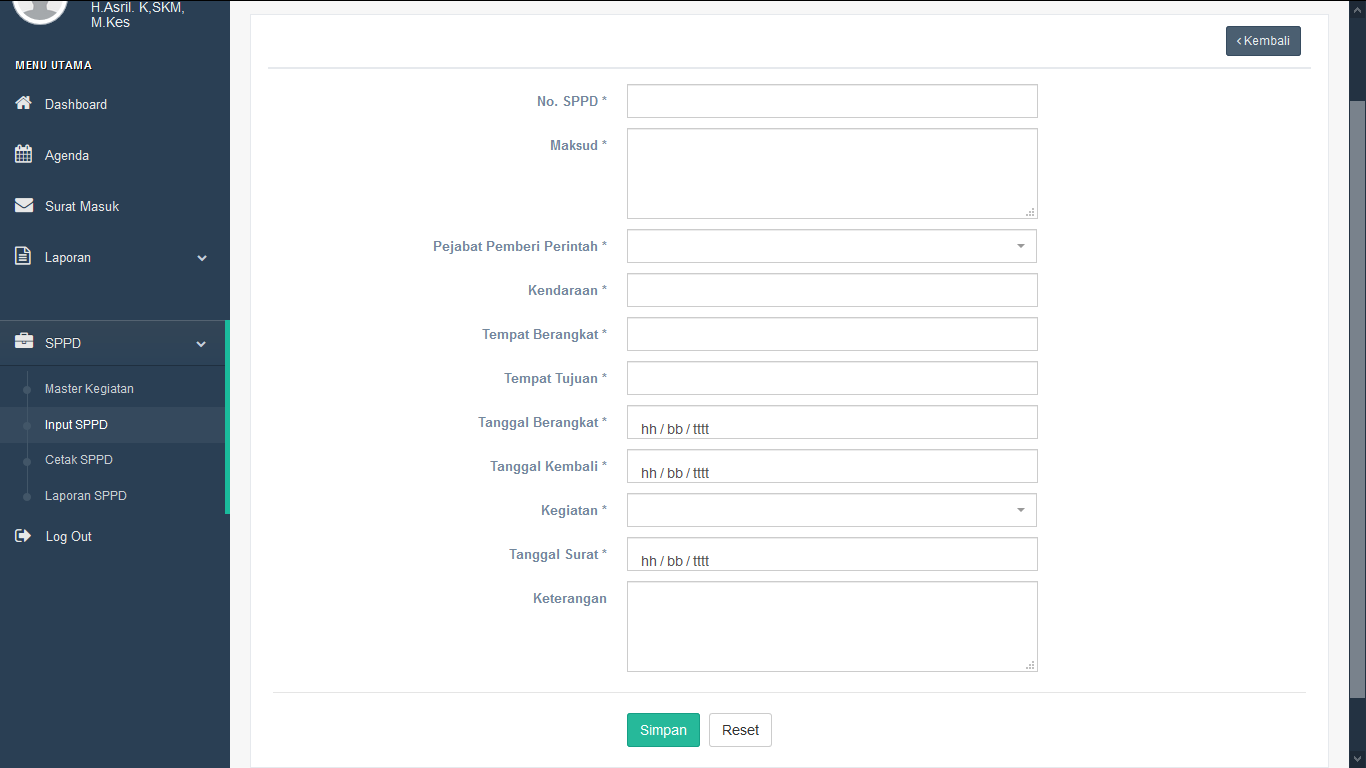
\includegraphics [height= 7cm, width=11cm]{konten/gambar/UISistemSurat/Kadis/0.15.InputDataSPPD.png}
			\caption{Input Data SPPD Kadis}
			\label{InputDataSPPDKadis}
		\end{figure}
		
		\item Cetak SPPD
		
		Berikut adalah tampilan Cetak SPPD Kadis dapat dilihat pada \pic~\ref{CetakSPPDKadis}
		
		\begin{figure}
			\centering
			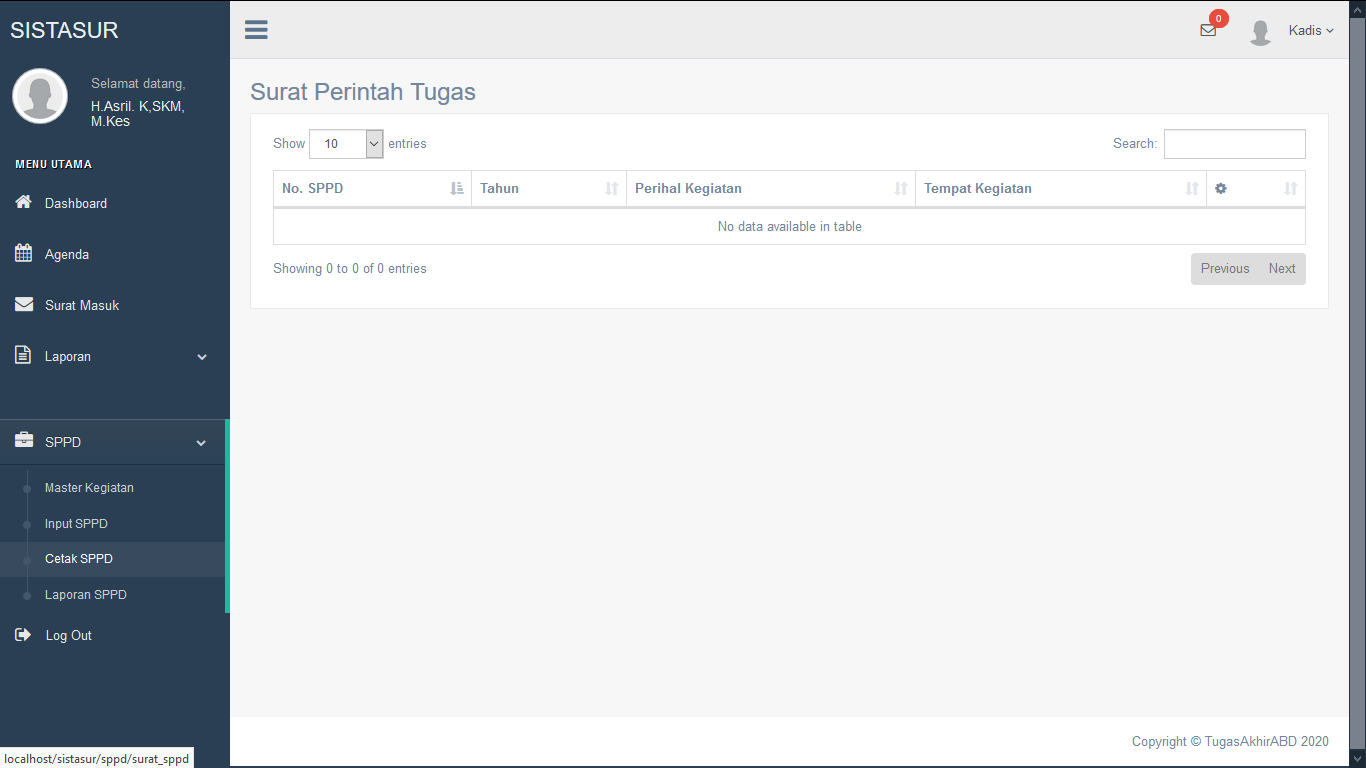
\includegraphics [height= 7cm, width=11cm]{konten/gambar/UISistemSurat/Kadis/0.16.CetakSPPD.png}
			\caption{Cetak SPPD Kadis}
			\label{CetakSPPDKadis}
		\end{figure}
		
		\item Rekap SPPD
		
		Berikut adalah tampilan Rekap SPPD Kadis dapat dilihat pada \pic~\ref{RekapSPPDKadis}
		
		\begin{figure}
			\centering
			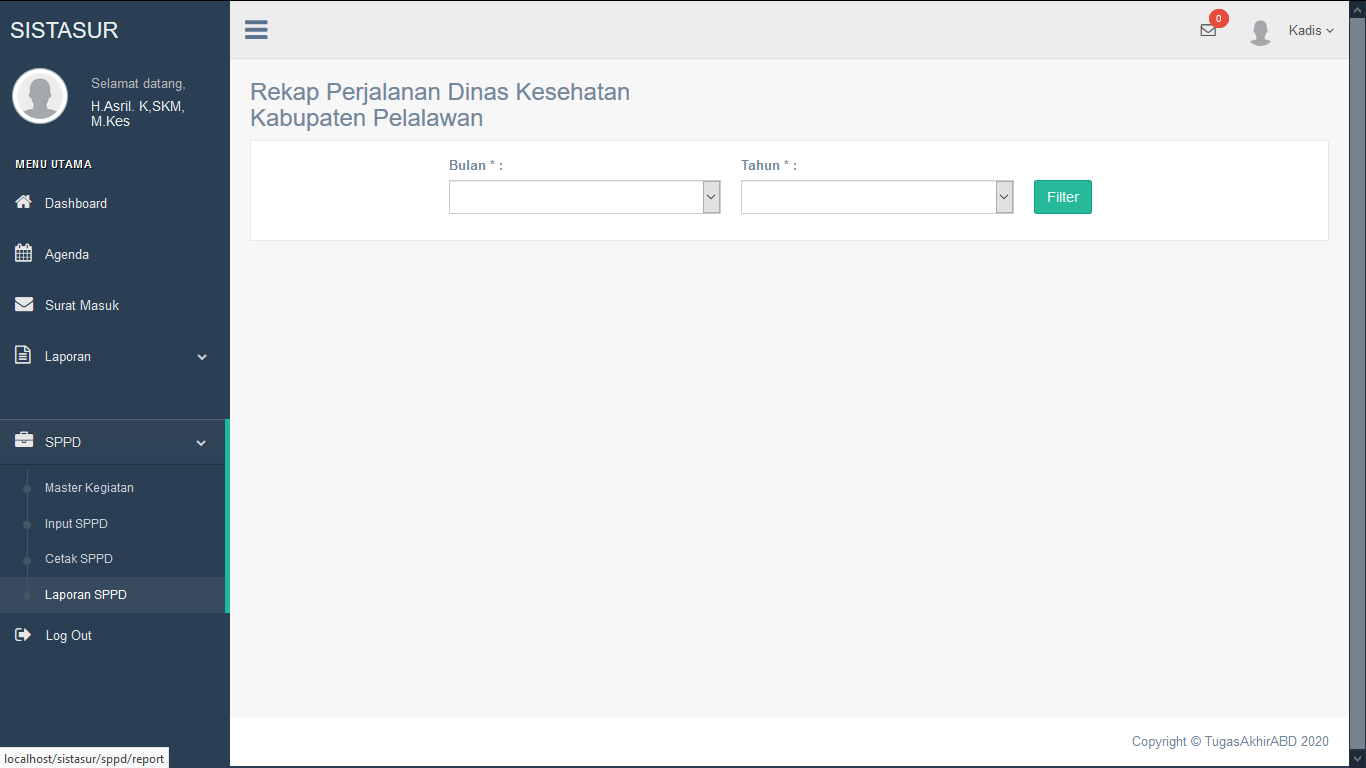
\includegraphics [height= 7cm, width=11cm]{konten/gambar/UISistemSurat/Kadis/0.17.RekapSPPD.png}
			\caption{Rekap SPPD Kadis}
			\label{RekapSPPDKadis}
		\end{figure}
	\end{enumerate}
	
	\item \textbf{Pengagenda}
	
	\begin{enumerate}
		\item Halaman Dashboard
		
		Berikut Adalah Halaman Dashboard yang dapat dilihat pada \pic~\ref{Dashboardpengagenda}
		
		\begin{figure}
			\centering
			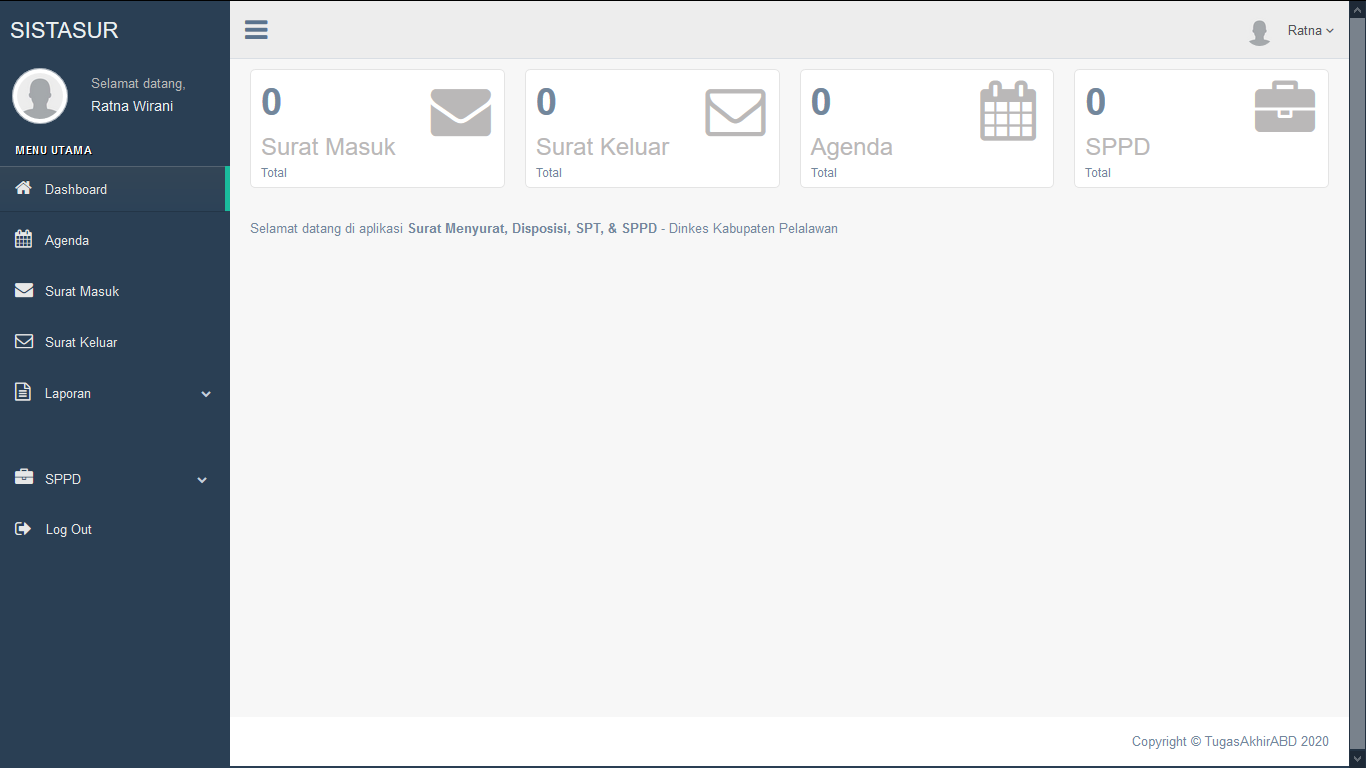
\includegraphics [height= 7cm, width=11cm]{konten/gambar/UISistemSurat/Pengagenda/0.1.Dashboard.png}
			\caption{Dashboard Pengagenda}
			\label{Dashboardpengagenda}
		\end{figure}
		
		\item Detail Profile Pengagenda
		
		Berikut Adalah Detail Profile Pengagenda yang dapat dilihat pada \pic~\ref{DetailProfilePengagenda}
		
		\begin{figure}
			\centering
			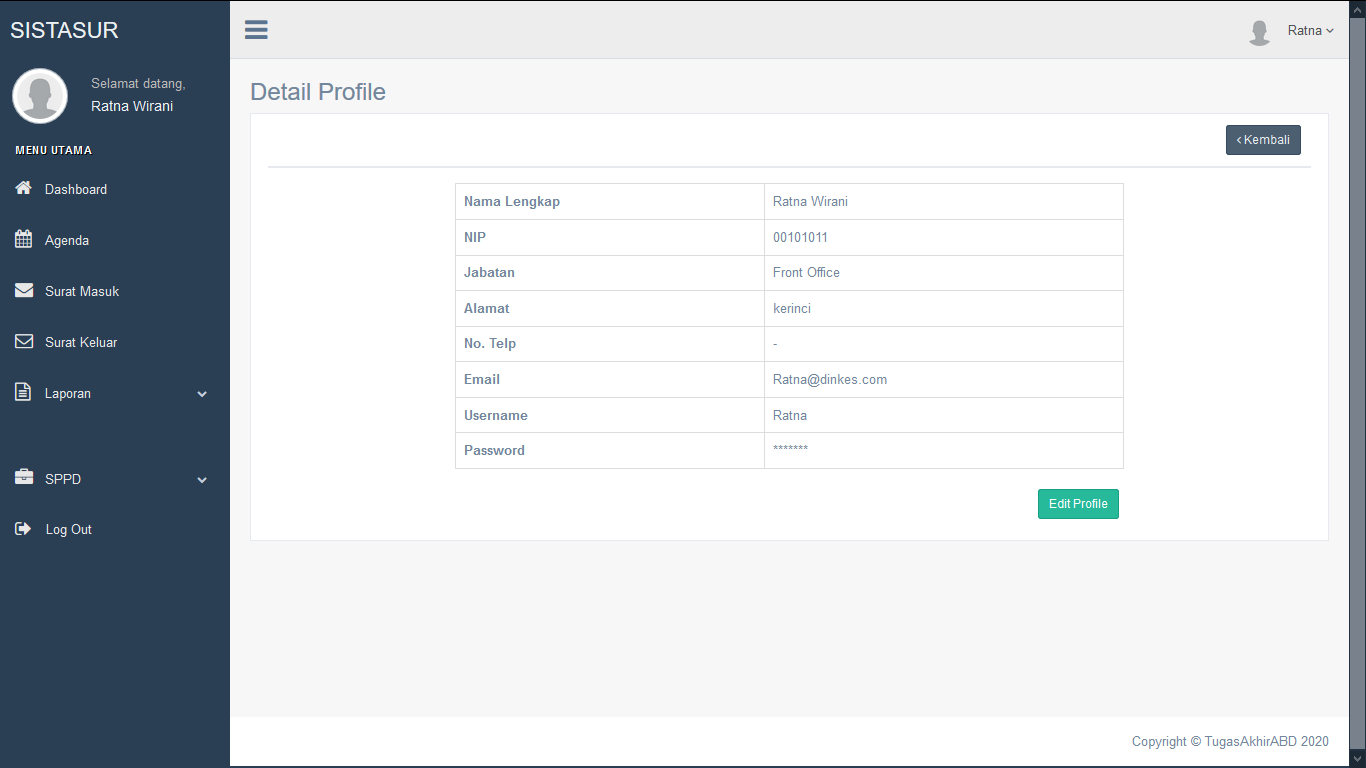
\includegraphics [height= 7cm, width=11cm]{konten/gambar/UISistemSurat/Pengagenda/0.2.DetailProfile.png}
			\caption{Detail Profile Pengagenda}
			\label{DetailProfilePengagenda}
		\end{figure}
		
		\item Lihat Master Agenda Pengagenda
		
		Berikut Adalah Lihat Master Agenda Pengagenda yang dapat dilihat pada \pic~\ref{LihatMasterAgendaPengagenda}
		
		\begin{figure}
			\centering
			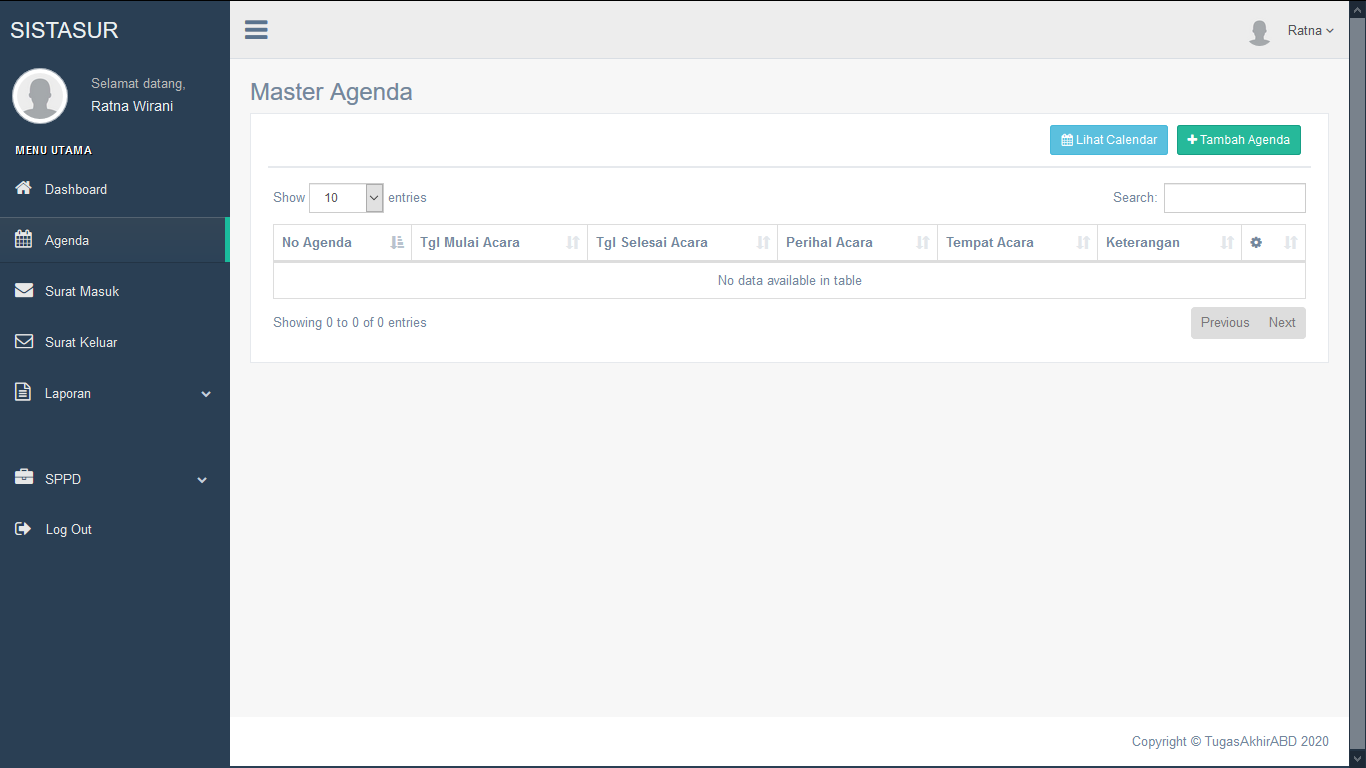
\includegraphics [height= 7cm, width=11cm]{konten/gambar/UISistemSurat/Pengagenda/0.3.LihatMasterAgenda.png}
			\caption{Lihat Master Agenda Pengagenda}
			\label{LihatMasterAgendaPengagenda}
		\end{figure}
		
		\item Lihat Master Agenda Bulanan Pengagenda
		
		Berikut Adalah Lihat Master Agenda Bulanan Pengagenda yang dapat dilihat pada \pic~\ref{LihatMasterAgendaBulananPengagenda}
		
		\begin{figure}
			\centering
			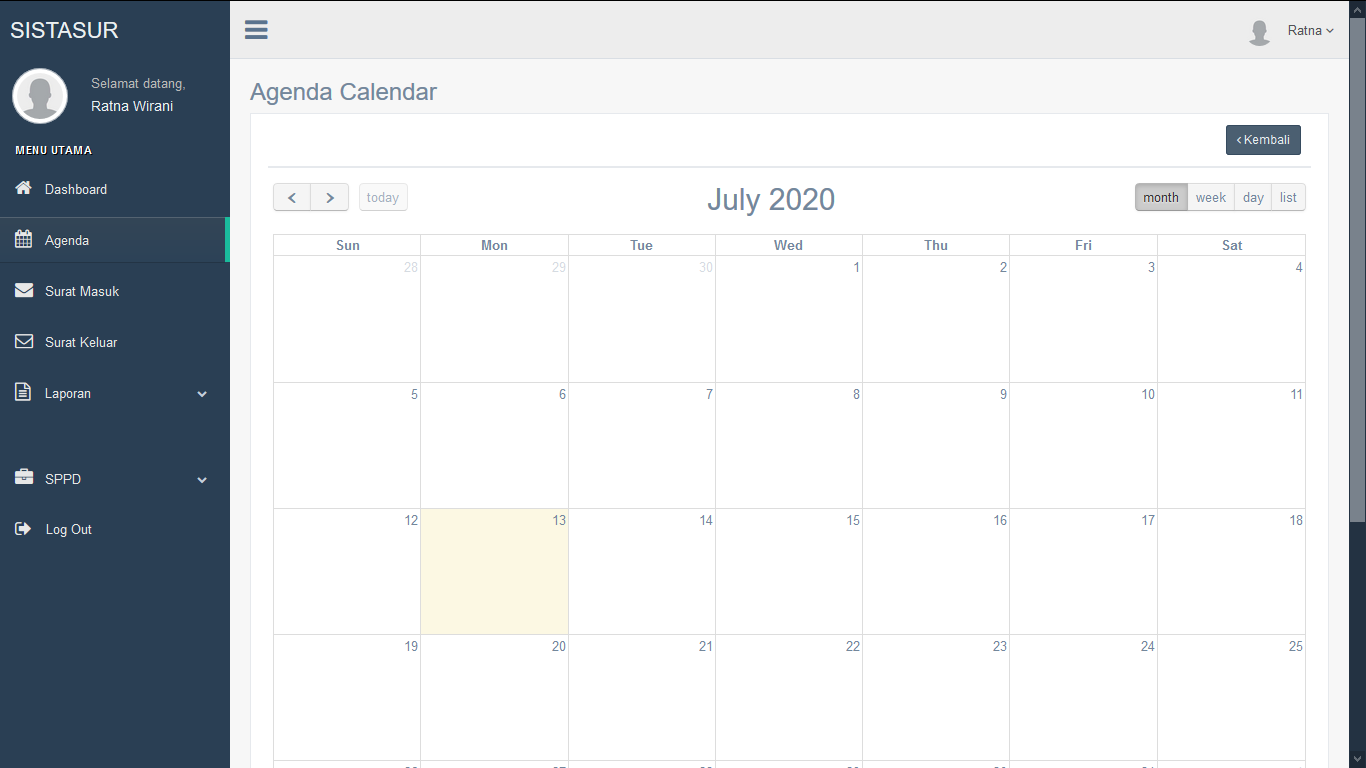
\includegraphics [height= 7cm, width=11cm]{konten/gambar/UISistemSurat/Pengagenda/0.4.LihatMasterAgendaBulanan.png}
			\caption{Lihat Master Agenda Bulanan Pengagenda}
			\label{LihatMasterAgendaBulananPengagenda}
		\end{figure}
		
		\item Lihat Master Agenda Mingguan Pengagenda
		
		Berikut Adalah Lihat Master Agenda Mingguan Pengagenda yang dapat dilihat pada \pic~\ref{LihatMasterAgendaMingguanPengagenda}
		
		\begin{figure}
			\centering
			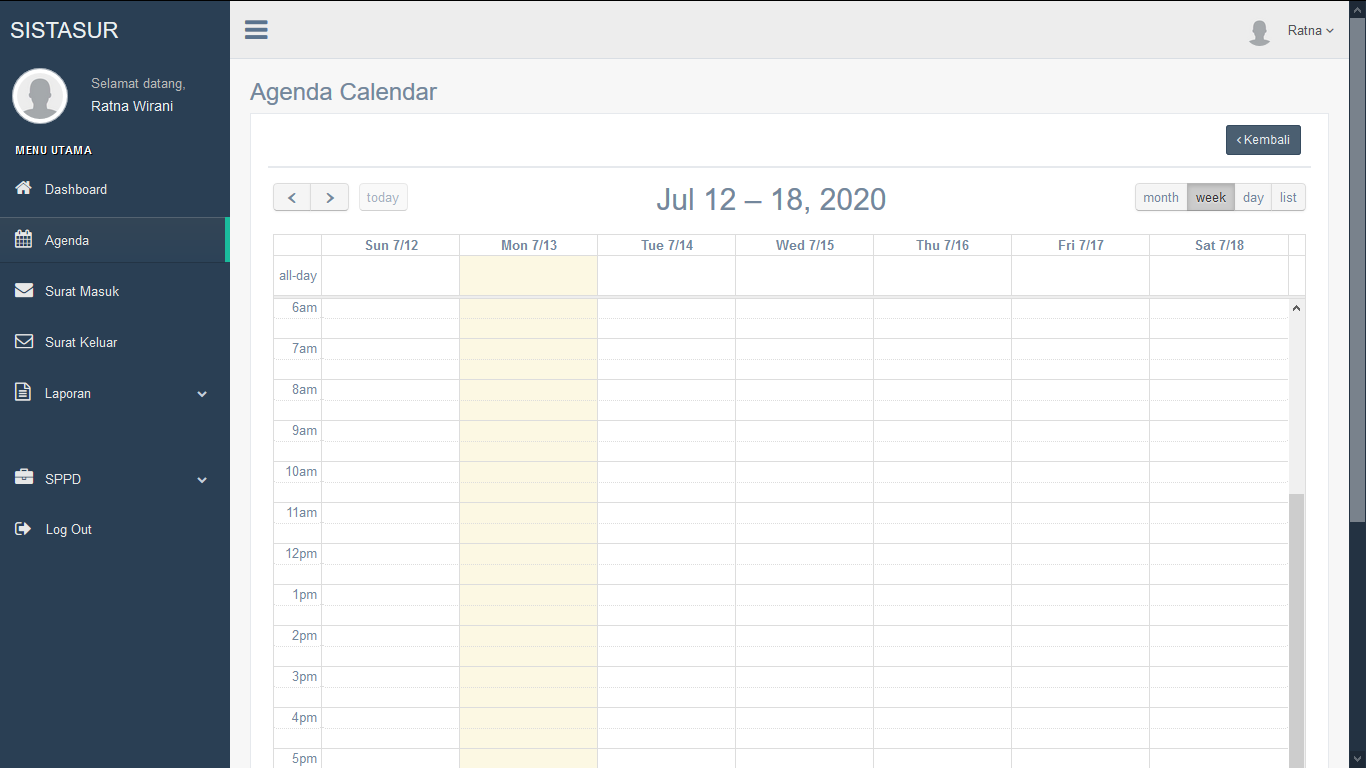
\includegraphics [height= 7cm, width=11cm]{konten/gambar/UISistemSurat/Pengagenda/0.5.LihatMasterAgendaMingguan.png}
			\caption{Lihat Master Agenda Mingguan Pengagenda}
			\label{LihatMasterAgendaMingguanPengagenda}
		\end{figure}
		
		
		\item Lihat Master Agenda Harian Pengagenda
		
		Berikut Adalah Lihat Master Agenda Harian Pengagenda yang dapat dilihat pada \pic~\ref{LihatMasterAgendaHarianPengagenda}
		
		\begin{figure}
			\centering
			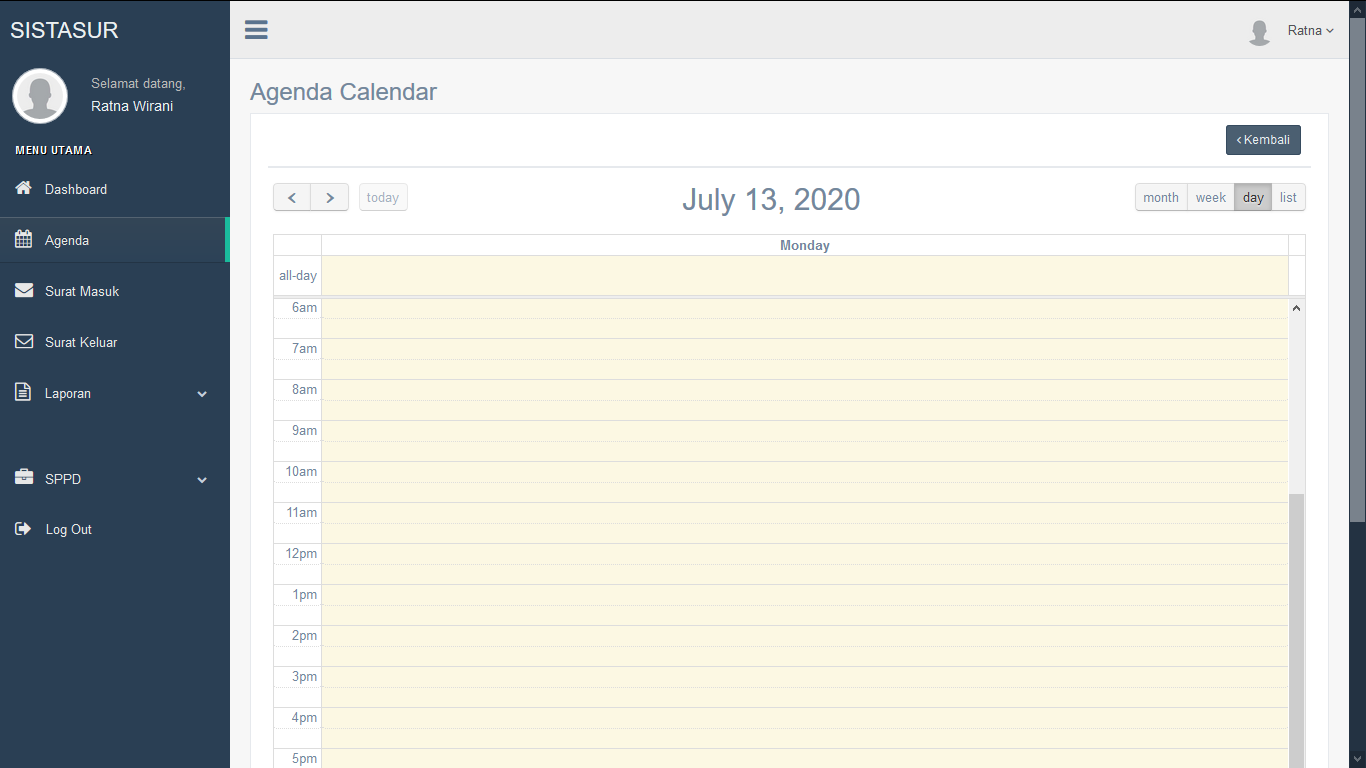
\includegraphics [height= 7cm, width=11cm]{konten/gambar/UISistemSurat/Pengagenda/0.6.LihatMasterAgendaHarian.png}
			\caption{Lihat Master Agenda Harian Pengagenda}
			\label{LihatMasterAgendaHarianPengagenda}
		\end{figure}
		
		
		\item Tambah Agenda Pengagenda
		
		Berikut Adalah Tambah Agenda Pengagenda yang dapat dilihat pada \pic~\ref{TambahAgendaPengagenda}
		
		\begin{figure}
			\centering
			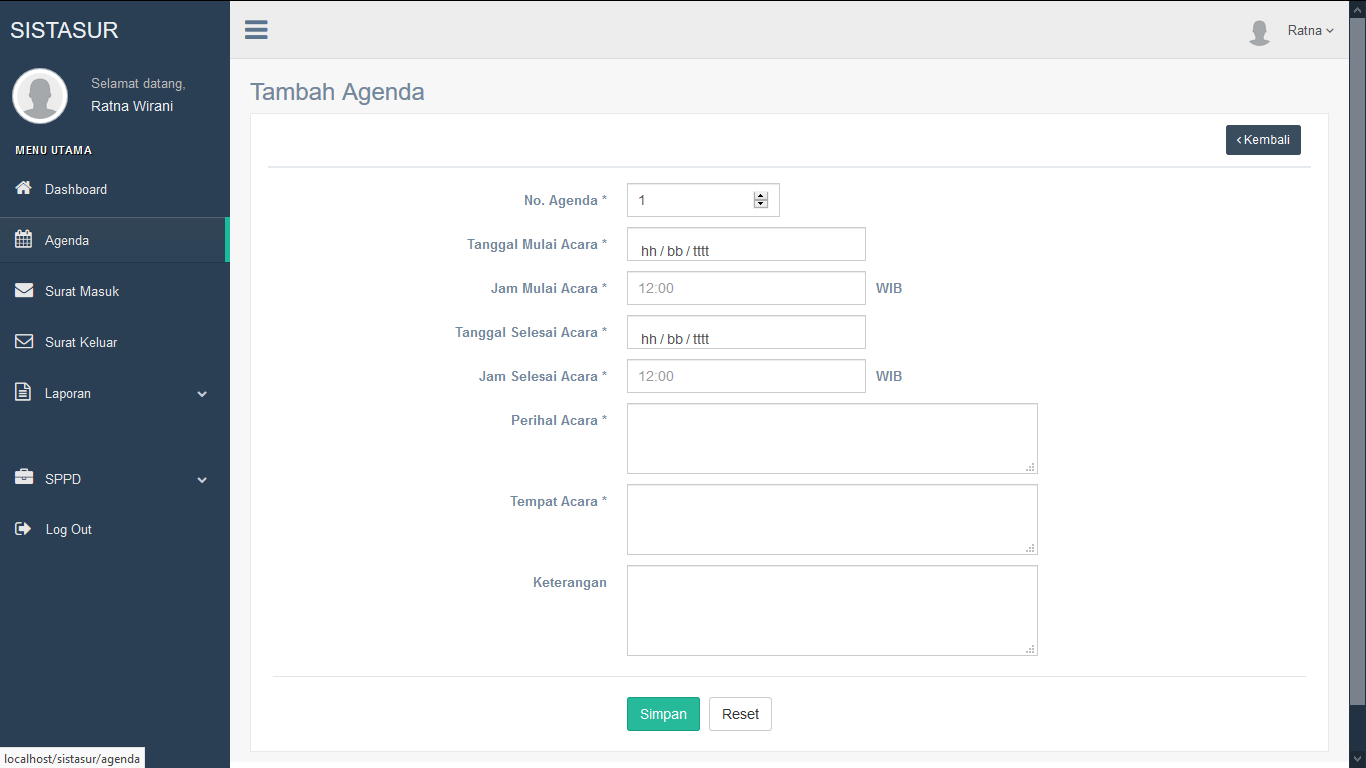
\includegraphics [height= 7cm, width=11cm]{konten/gambar/UISistemSurat/Pengagenda/0.7.TambahAgenda.png}
			\caption{Tambah Agenda Pengagenda}
			\label{TambahAgendaPengagenda}
		\end{figure}
		
		
		\item Tambah Data Surat Masuk Pengagenda
		
		Berikut Adalah Tambah Data Surat Masuk Pengagenda yang dapat dilihat pada \pic~\ref{TambahDataSuratMasukPengagenda}
		
		\begin{figure}
			\centering
			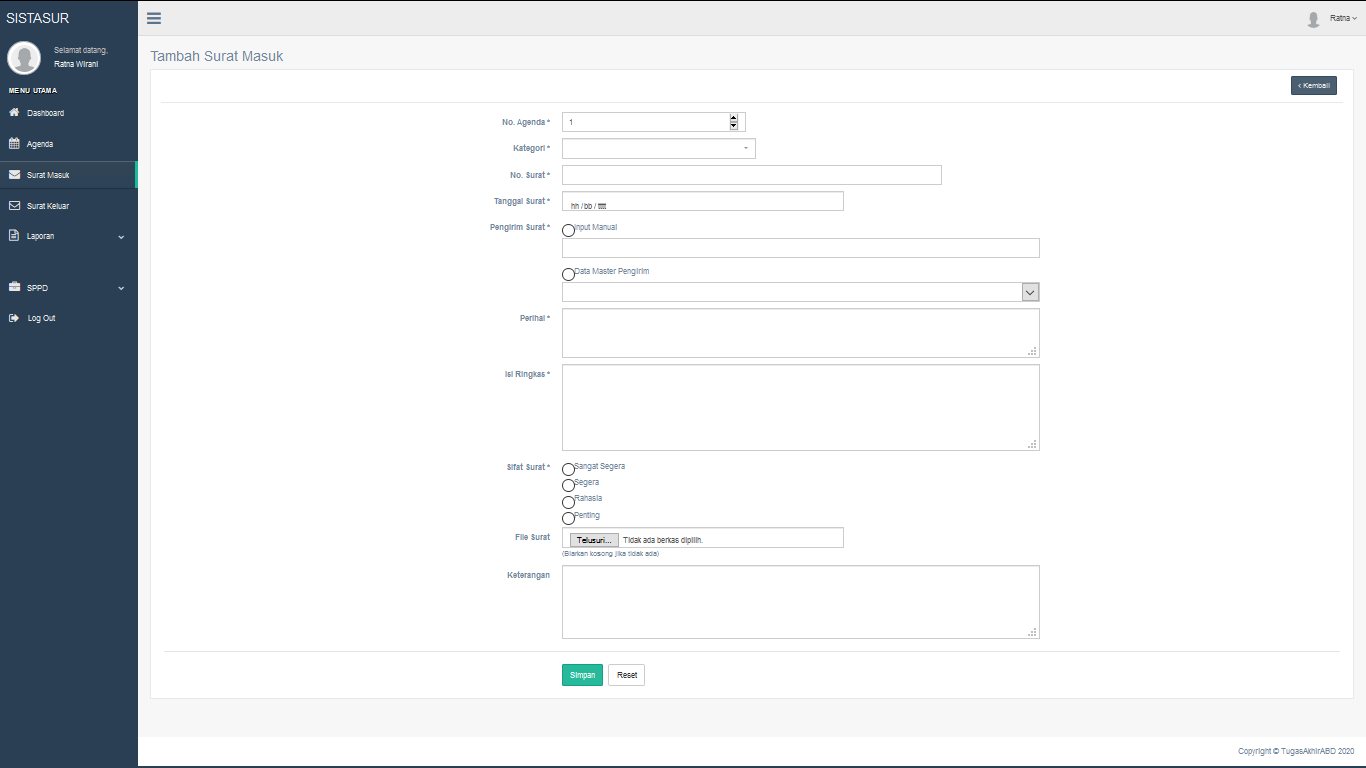
\includegraphics [height= 7cm, width=11cm]{konten/gambar/UISistemSurat/Pengagenda/0.9.TambahDataSuratMasuk.png}
			\caption{Tambah Data Surat Masuk Pengagenda}
			\label{TambahDataSuratMasukPengagenda}
		\end{figure}
		
		
		\item Lihat Data Surat Masuk Pengagenda
		
		Berikut Adalah Lihat Data Surat Masuk Pengagenda yang dapat dilihat pada \pic~\ref{LihatDataSuratMasukPengagenda}
		
		\begin{figure}
			\centering
			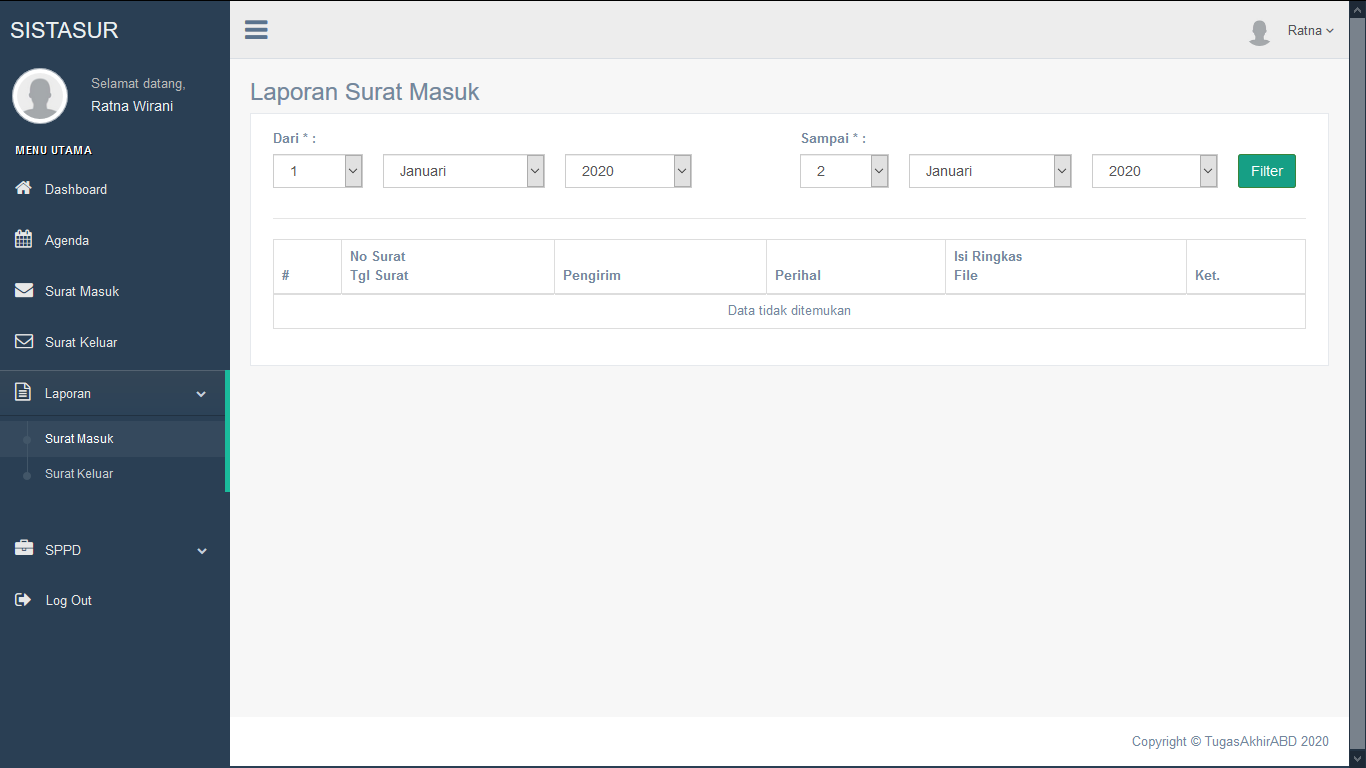
\includegraphics [height= 7cm, width=11cm]{konten/gambar/UISistemSurat/Pengagenda/0.10.LihatDataSuratMasuk.png}
			\caption{Lihat Data Surat Masuk Pengagenda}
			\label{LihatDataSuratMasukPengagenda}
		\end{figure}
		
		
		\item Lihat Data Surat Keluar Pengagenda
		
		Berikut Adalah Lihat Data Surat Keluar Pengagenda yang dapat dilihat pada \pic~\ref{LihatDataSuratKeluarPengagenda}
		
		\begin{figure}
			\centering
			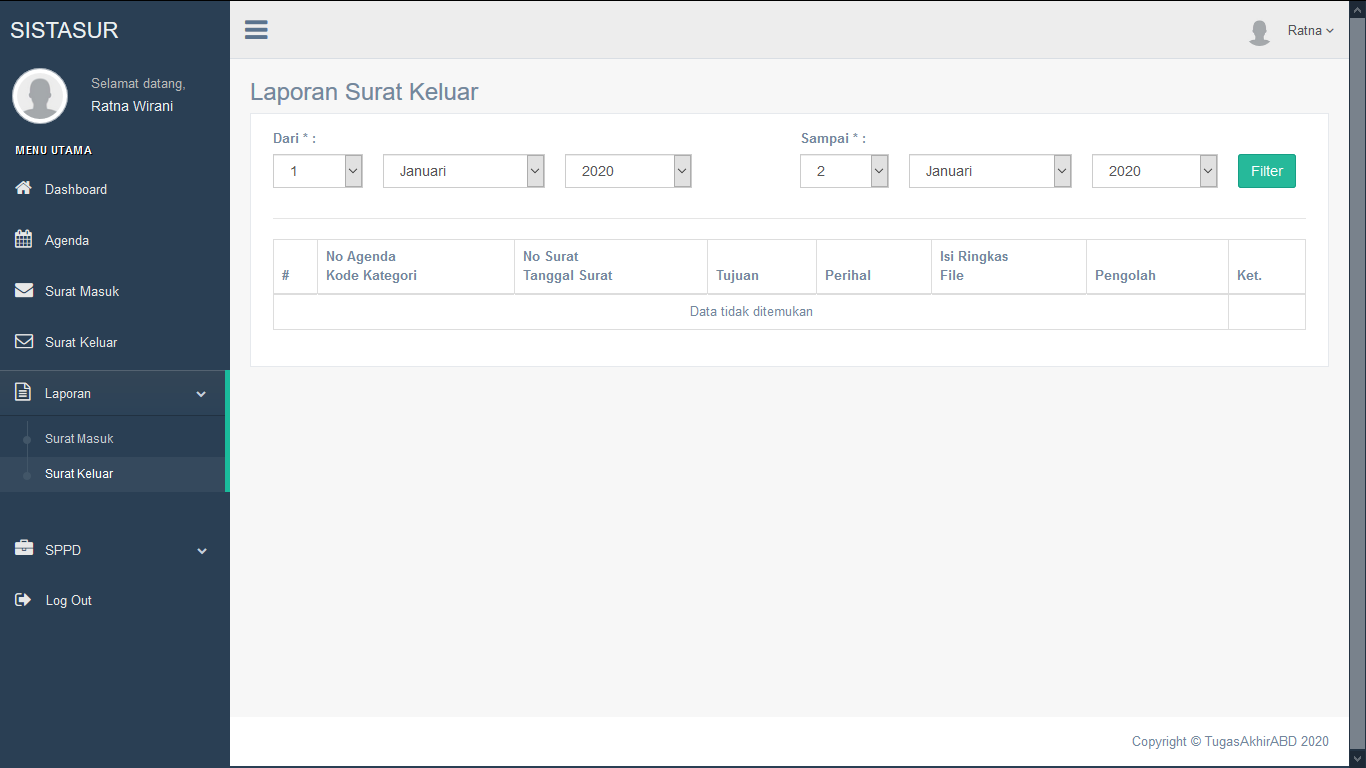
\includegraphics [height= 7cm, width=11cm]{konten/gambar/UISistemSurat/Pengagenda/0.11.LihatDataSuratKeluar.png}
			\caption{Lihat Data Surat Keluar Pengagenda}
			\label{LihatDataSuratKeluarPengagenda}
		\end{figure}
		
		
		\item Data Master DPA Pengagenda
		
		Berikut Adalah Data Master DPA Pengagenda yang dapat dilihat pada \pic~\ref{DataMasterDPAPengagenda}
		
		\begin{figure}
			\centering
			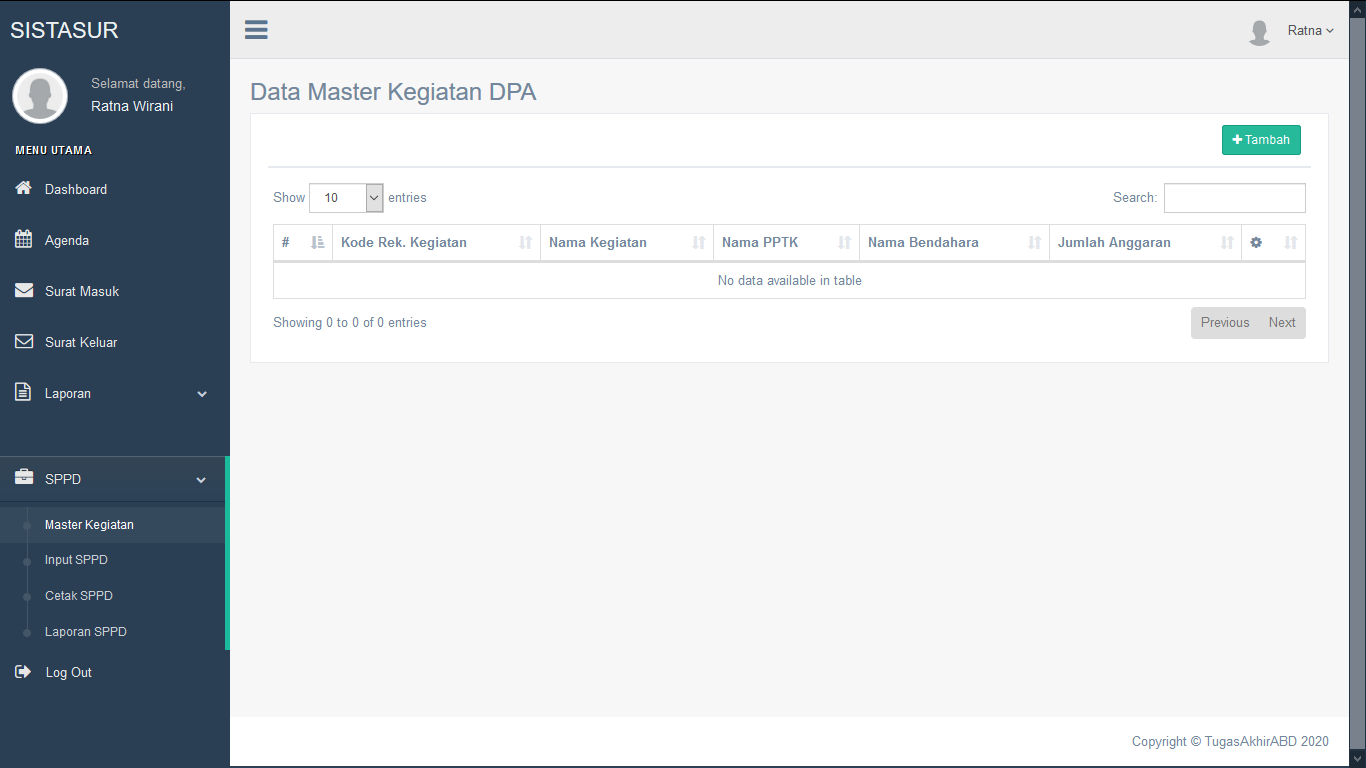
\includegraphics [height= 7cm, width=11cm]{konten/gambar/UISistemSurat/Pengagenda/0.12.DataMasterDPA.png}
			\caption{Data Master DPA Pengagenda}
			\label{DataMasterDPAPengagenda}
		\end{figure}
		
		
		\item Input Master DPA Pengagenda
		
		Berikut Adalah Input Master DPA Pengagenda yang dapat dilihat pada \pic~\ref{InputMasterDPAPengagenda}
		
		\begin{figure}
			\centering
			\includegraphics [height= 7cm, width=11cm]{konten/gambar/UISistemSurat/Pengagenda/0.13.InputMasterDPA.png}
			\caption{Input Master DPA Pengagenda}
			\label{InputMasterDPAPengagenda}
		\end{figure}
		
		
		\item Lihat Data SPPD Pengagenda
		
		Berikut Adalah Lihat Data SPPD Pengagenda yang dapat dilihat pada \pic~\ref{LihatDataSPPDPengagenda}
		
		\begin{figure}
			\centering
			\includegraphics [height= 7cm, width=11cm]{konten/gambar/UISistemSurat/Pengagenda/0.14.LihatDataSPPD.png}
			\caption{Lihat Data SPPD Pengagenda}
			\label{LihatDataSPPDPengagenda}
		\end{figure}
		
		
		\item Tambah Data SPPD Pengagenda
		
		Berikut Adalah Tambah Data SPPD Pengagenda yang dapat dilihat pada \pic~\ref{TambahDataSPPDPengagenda}
		
		\begin{figure}
			\centering
			\includegraphics [height= 7cm, width=11cm]{konten/gambar/UISistemSurat/Pengagenda/0.15.TambahDataSPPD.png}
			\caption{Tambah Data SPPD Pengagenda}
			\label{TambahDataSPPDPengagenda}
		\end{figure}
		
		
		\item Cetak Data SPPD Pengagenda
		
		Berikut Adalah Cetak Data SPPD Pengagenda yang dapat dilihat pada \pic~\ref{CetakDataSPPDPengagenda}
		
		\begin{figure}
			\centering
			\includegraphics [height= 7cm, width=11cm]{konten/gambar/UISistemSurat/Pengagenda/0.16.CetakDataSPPD.png}
			\caption{Cetak Data SPPD Pengagenda}
			\label{CetakDataSPPDPengagenda}
		\end{figure}
		
		
		\item Rekap Data SPPD 
		
		Berikut Adalah Rekap Data SPPD yang dapat dilihat pada \pic~\ref{RekapDataSPPD}
		
		\begin{figure}
			\centering
			\includegraphics [height= 7cm, width=11cm]{konten/gambar/UISistemSurat/Pengagenda/0.17.RekapDataSPPD.png}
			\caption{Rekap Data SPPD}
			\label{RekapDataSPPD}
		\end{figure}
		
	\end{enumerate}
	
	\item \textbf{Pegawai}
	
	\begin{enumerate}
		\item Halaman Dashboard
		
		Berikut Adalah Halaman Dashboard yang dapat dilihat pada \pic~\ref{DashboardPegawai}
		
		\begin{figure}
			\centering
			\includegraphics [height= 7cm, width=11cm]{konten/gambar/UISistemSurat/Pegawai/0.1.Dashboard.png}
			\caption{DashboardPegawai}
			\label{DashboardPegawai}
		\end{figure}
		
		\item Notifikasi Disposisi Pegawai
		
		Berikut Adalah NotifikasiDisposisiPegawai yang dapat dilihat pada \pic~\ref{NotifikasiDisposisiPegawai}
		
		\begin{figure}
			\centering
			\includegraphics [height= 7cm, width=11cm]{konten/gambar/UISistemSurat/Pegawai/0.2NotifikasiDisposisi.png}
			\caption{NotifikasiDisposisiPegawai}
			\label{NotifikasiDisposisiPegawai}
		\end{figure}
		
		\item Detail Profile Pegawai
		
		Berikut Adalah Detail Profile Pegawai yang dapat dilihat pada \pic~\ref{DetailProfilePegawai}
		
		\begin{figure}
			\centering
			\includegraphics [height= 7cm, width=11cm]{konten/gambar/UISistemSurat/Pegawai/0.3.DetailProfile.png}
			\caption{Detail Profile Pegawai}
			\label{DetailProfilePegawai}
		\end{figure}
		
		
		\item Data Surat Masuk Pegawai
		
		Berikut Adalah Data Surat Masuk Pegawai yang dapat dilihat pada \pic~\ref{DataSuratMasukPegawai}
		
		\begin{figure}
			\centering
			\includegraphics [height= 7cm, width=11cm]{konten/gambar/UISistemSurat/Pegawai/0.4.DataSuratMasuk.png}
			\caption{Data Surat Masuk Pegawai}
			\label{DataSuratMasukPegawai}
		\end{figure}
		
		\item Laporan Surat Masuk Pegawai
		
		Berikut Adalah Laporan Surat Masuk Pegawai yang dapat dilihat pada \pic~\ref{LaporanSuratMasukPegawai}
		
		\begin{figure}
			\centering
			\includegraphics [height= 7cm, width=11cm]{konten/gambar/UISistemSurat/Pegawai/0.5.LaporanSuratMasuk.png}
			\caption{Laporan Surat Masuk Pegawai}
			\label{LaporanSuratMasukPegawai}
		\end{figure}
		
		\item Laporan Surat Keluar Pegawai
		
		Berikut Adalah Laporan Surat Keluar Pegawai yang dapat dilihat pada \pic~\ref{LaporanSuratKeluarPegawai}
		
		\begin{figure}
			\centering
			\includegraphics [height= 7cm, width=11cm]{konten/gambar/UISistemSurat/Pegawai/0.6.LaporanSuratKeluar.png}
			\caption{Laporan Surat Keluar Pegawai}
			\label{LaporanSuratKeluarPegawai}
		\end{figure}
		
		\item Lihat Data Master Kegiatan DPA Pegawai
		
		Berikut Adalah Lihat Data Master Kegiatan DPA Pegawai yang dapat dilihat pada \pic~\ref{LihatDataMasterKegiatanDPAPegawai}
		
		\begin{figure}
			\centering
			\includegraphics [height= 7cm, width=11cm]{konten/gambar/UISistemSurat/Pegawai/0.7.LihatDataMasterKegiatanDPA.png}
			\caption{Lihat Data Master Kegiatan DPA Pegawai}
			\label{LihatDataMasterKegiatanDPAPegawai}
		\end{figure}
		
		\item Tambah Data Kegiatan DPA Pegawai
		
		Berikut Adalah Tambah Data Kegiatan DPA Pegawai yang dapat dilihat pada \pic~\ref{TambahDataKegiatanDPAPegawai}
		
		\begin{figure}
			\centering
			\includegraphics [height= 7cm, width=11cm]{konten/gambar/UISistemSurat/Pegawai/0.8.TambahDataKegiatanDPA.png}
			\caption{Tambah Data Kegiatan DPA Pegawai}
			\label{TambahDataKegiatanDPAPegawai}
		\end{figure}
		
		\item Lihat Data SPPD Pegawai
		
		Berikut Adalah Lihat Data SPPD Pegawai yang dapat dilihat pada \pic~\ref{LihatDataSPPDPegawai}
		
		\begin{figure}
			\centering
			\includegraphics [height= 7cm, width=11cm]{konten/gambar/UISistemSurat/Pegawai/0.9.LihatDataSPPD.png}
			\caption{Lihat Data SPPD Pegawai}
			\label{LihatDataSPPDPegawai}
		\end{figure}
		
		
		\item Tambah Data SPPD Pegawai
		
		Berikut Adalah Tambah Data SPPD Pegawai yang dapat dilihat pada \pic~\ref{TambahDataSPPDPegawai}
		
		\begin{figure}
			\centering
			\includegraphics [height= 7cm, width=11cm]{konten/gambar/UISistemSurat/Pegawai/0.10.TambahDataSPPD.png}
			\caption{Tambah Data SPPD Pegawai}
			\label{TambahDataSPPDPegawai}
		\end{figure}
		
		
		\item Cetak SPPD Pegawai
		
		Berikut Adalah Cetak SPPD Pegawai yang dapat dilihat pada \pic~\ref{CetakSPPDPegawai}
		
		\begin{figure}
			\centering
			\includegraphics [height= 7cm, width=11cm]{konten/gambar/UISistemSurat/Pegawai/0.11.CetakSPPD.png}
			\caption{Cetak SPPD Pegawai}
			\label{CetakSPPDPegawai}
		\end{figure}
		
		
		\item Rekap SPPD Pegawai
		
		Berikut Adalah Rekap SPPD Pegawai yang dapat dilihat pada \pic~\ref{RekapSPPDPegawai}
		
		\begin{figure}
			\centering
			\includegraphics [height= 7cm, width=11cm]{konten/gambar/UISistemSurat/Pegawai/0.12.RekapSPPD.png}
			\caption{Rekap SPPD Pegawai}
			\label{RekapSPPDPegawai}
		\end{figure}
	\end{enumerate}
	
\end{enumerate}


\section{Pengujian Sistem}
Setelah tahapan dari analisa serta perancangan selesai dilaksanakan maka dilanjutkan ke
tahapan dari implementasi dan pengujian. Adapun tahapan ini dilakukan pengujian terhadap fitur-
fitur yang tersedia pada aplikasi, selanjutnya dilakukan pengamatan dari hasil pengujian tersebut
sehingga diketahui fitur-fitur yang masih memiliki kekurangan untuk diambil kesimpulan. Pengujian
aplikasi ini menggunakan perangkat PC dan Laptop.

\subsection {\textit{Blackbox Testing}}.


Pengujian yang dilakukan terhadap aplikasi adalah menggunakan metode \textit{blackbox testing}. Aplikasi ini dari sisi spesifikasi secara fungsional tanpa menguji desain serta kode program di dalamnya. Tujuan dari pengujian ini ditujukan untukmengetahui fungsi-fungsi, masukan serta keluaran dari aplikasi sesuai dengan spesifikasi yang diperlukan.
\begin{enumerate}
	\item \textit{Blackbox Testing} Bagian Admin
	
	Berikut adalah tabel \textit{Blackbox} pada \textit{role} Admin. Dapat dilihat pada \tab~\ref{blackboxtesting}
	 {\fontsize{10pt}{12pt}\selectfont
	\renewcommand\namaTabel{Hasil pengujian \textit{blackbox testing} Admin}
		
	\begin{longtable}{p{0.5cm} p{4cm} p{4cm} p{0.5cm} p{1cm}}
		\caption{Tabel \textit{Blackbox} Admin}
		\label{blackboxtesting}\\ 
		\hline
		\multicolumn{1}{c}{\multirow{2}{*}{\textbf{No}}} & \multicolumn{1}{c}{\multirow{2}{*}{\textbf{Pengujian}}} & \multicolumn{1}{c}{\multirow{2}{*}{\textbf{Interface yang Diharapkan}}} & \multicolumn{2}{c}{\textbf{Hasil Uji}} \\ \cline{4-5} 
		\multicolumn{1}{c}{} & \multicolumn{1}{c}{} & \multicolumn{1}{c}{} & \multicolumn{1}{c}{\textbf{Berhasil}} & \multicolumn{1}{c}{\textbf{Tidak Berhasil}} \\ \hline
		\endfirsthead
		%
		\multicolumn{5}{c}{\tablename\ \thetable\ \namaTabel \space (Tabel
			lanjutan...)} \\
		\hline
		\multicolumn{1}{c}{\multirow{2}{*}{\textbf{No}}} & \multicolumn{1}{c}{\multirow{2}{*}{\textbf{Pengujian}}} & \multicolumn{1}{c}{\multirow{2}{*}{\textbf{Interface yang Diharapkan}}} & \multicolumn{2}{c}{\textbf{Hasil Uji}} \\ \cline{4-5} 
		\multicolumn{1}{c}{} & \multicolumn{1}{c}{} & \multicolumn{1}{c}{} & \multicolumn{1}{c}{\textbf{Berhasil}} & \multicolumn{1}{c}{\textbf{Tidak Berhasil}} \\ \hline
		\endhead
		%
		1 & \textit{Admin} tidak mengisi \textit{username} dan \textit{password} & Tampil notifikasi \textit{username} atau \textit{password} tidak boleh kosong & \checkmark & -\\
		2 & \textit{Username} atau \textit{password} yang dimasukkan salah & Tampil notifikasi \textit{username} atau \textit{password} yang dimasukkan salah & \checkmark & -\\
		3 & \textit{Username} dan \textit{password} yang di masukkan benar & Masuk ke halaman \textit{dashboard Administrator} & \checkmark & -\\
		4 & \textit{Admin} Mengklik menu Edit Profil  & Data edit profil ditampilkan & \checkmark & -\\
		5 & \textit{Admin} Mengubah Data pada  menu Edit Profil  & Data edit profil disimpan ke \textit{Database} & \checkmark & -\\
		6 & \textit{Admin} Mengklik Data Golongan Pegawai & Data Golongan Pegawai ditampilkan & \checkmark & -\\
		7 & \textit{Admin} Menambahkan Data Golongan Pegawai & Data Golongan Pegawai disimpan ke \textit{Database}  & \checkmark & -\\
		8 & \textit{Admin} mengisi Data Golongan Pegawai & Data jadwal berhasil ditambahkan & \checkmark & -\\
		9 & \textit{Admin} mengklik Lihat Master Jabatan Pegawai & Data Lihat Master Jabatan Pegawai ditampilkan & \checkmark & -\\
		10 & \textit{Admin} Menambahkan Jabatan Pegawai & Data Jabatan Pegawai disimpan ke \textit{Database}  & \checkmark & -\\
		11 & \textit{Admin} Mengklik Data Pegawai & Data Pegawai ditampilkan  & \checkmark & -\\
		12 & \textit{Admin} Menambahkan Data Pegawai & Data Pegawai berhasil disimpan ke \textit{database}  & \checkmark & -\\
		13 & \textit{Admin} Mengklik Struktur Organisasi & Data Struktur Organisasi Berhasil ditampilkan  & \checkmark & -\\
		14 & \textit{Admin} Mengklik Lihat Kategori Surat & Lihat Kategori Surat Berhasil ditampilkan  & \checkmark & -\\
		15 & \textit{Admin} Mengklik Tambah Kategori Surat & Kategori Surat Berhasil disimpan ke \textit{Database}  & \checkmark & -\\
		16 & \textit{Admin} Mengklik Lihat Master Pengirim Surat & Lihat Master Pengirim Surat Berhasil Ditampilkan  & \checkmark & -\\
		17 & \textit{Admin} Menambahkan Lihat Master Pengirim Surat & Lihat Master Pengirim Surat disimpan ke \textit{Database}  & \checkmark & -\\
		18 & \textit{Admin} Mengklik Tambah Data Pengirim Surat & Tambah Data Pengirim Surat Berhasil Ditampilkan  & \checkmark & -\\
		19 & \textit{Admin} Menambahkan Tambah Data Pengirim Surat & Data Pengirim Surat Berhasil disimpan ke \textit{Database}  & \checkmark & -\\
		20 & \textit{Admin} Mengklik Lihat Tujuan Surat Keluar & Kategori Surat Berhasil Ditampilkan  & \checkmark & -\\
		21 & \textit{Admin} Menambahkan Lihat Tujuan Surat Keluar & Kategori Surat Berhasil disimpan ke \textit{Database}  & \checkmark & -\\
		22 & \textit{Admin} Mengklik Tambah Data Tujuan Surat Keluar & Tambah Data Tujuan Surat Keluar ditampilkan  & \checkmark & -\\
		23 & \textit{Admin} Menambahkan Tambah Data Tujuan Surat Keluar & Tambah Data Tujuan Surat Keluar Berhasil disimpan ke \textit{Database}  & \checkmark & -\\
		24 & \textit{Admin} Mengklik Lihat Data Surat Masuk & Kategori Surat Berhasil Ditampilkan  & \checkmark & -\\
		25 & \textit{Admin} Menambahkan Lihat Data Surat Masuk & Lihat Data Surat Masuk Berhasil disimpan ke \textit{Database}  & \checkmark & -\\
		26 & \textit{Admin} Mengklik Lihat Data Surat Keluar & Lihat Data Surat Keluar Berhasil Ditampilkan  & \checkmark & -\\
		27 & \textit{Admin} Menambahkan Lihat Data Surat Keluar & Lihat Data Surat Keluar Berhasil disimpan ke \textit{Database}  & \checkmark & -\\
		28 & \textit{Admin} Mengklik Tambah Data SPPD & Tambah Data SPPD Berhasil Ditampilkan  & \checkmark & -\\
		29 & \textit{Admin} Menambahkan Tambah Data SPPD & Tambah Data SPPD Berhasil disimpan ke \textit{Database}  & \checkmark & -\\
		30 & \textit{Admin} Mengklik Tambah Data SPPD Master & Tambah Data SPPD Master Berhasil Ditampilkan  & \checkmark & -\\
		31 & \textit{Admin} Menambahkan Tambah Data SPPD Master & Tambah Data SPPD Master Berhasil disimpan ke \textit{Database}  & \checkmark & -\\
		32 & \textit{Admin} Mengklik Lihat Data SPPD & Lihat Data SPPD Berhasil Ditampilkan  & \checkmark & -\\
		33 & \textit{Admin} Menambahkan Lihat Data SPPD & Lihat Data SPPD Berhasil disimpan ke \textit{Database}  & \checkmark & -\\
		34 & \textit{Admin} Mengklik Cetak SPPD & Cetak SPPD Master Berhasil Ditampilkan  & \checkmark & -\\
		35 & \textit{Admin} MMengklik Cetak SPPD & Cetak SPPD Master Berhasil Dicetak  & \checkmark & -\\		
		36 & \textit{Admin} Mengklik Rekap Data SPPD & Rekap Data SPPD Berhasil Ditampilkan  & \checkmark & -\\
		37 & \textit{Admin} Menambahkan Rekap Data SPPD & Rekap Data SPPD Berhasil  & \checkmark & -\\
		38 & \textit{Admin} Mengklik Menu \textit{logout} & \textit{logout} Berhasil  & \checkmark & -\\\hline
		\end{longtable}}
	
	
	
	\item \textit{Blackbox Testing} Bagian Kepala Dinas
	
	Berikut adalah tabel \textit{Blackbox} pada \textit{role} Kepala Dinas. Dapat dilihat pada \tab~\ref{blackboxtesting2}
	{\fontsize{10pt}{12pt}\selectfont
		\renewcommand\namaTabel{Hasil pengujian \textit{blackbox testing} Kepala Dinas}
		
		\begin{longtable}{p{0.5cm} p{4cm} p{5cm} p{0.5cm} p{1cm}}
			\caption{Tabel \textit{Blackbox} Kepala Dinas}
			\label{blackboxtesting2}\\ 
			\hline
			\multicolumn{1}{c}{\multirow{2}{*}{\textbf{No}}} & \multicolumn{1}{c}{\multirow{2}{*}{\textbf{Pengujian}}} & \multicolumn{1}{c}{\multirow{2}{*}{\textbf{Interface yang Diharapkan}}} & \multicolumn{2}{c}{\textbf{Hasil Uji}} \\ \cline{4-5} 
			\multicolumn{1}{c}{} & \multicolumn{1}{c}{} & \multicolumn{1}{c}{} & \multicolumn{1}{c}{\textbf{Berhasil}} & \multicolumn{1}{c}{\textbf{Tidak Berhasil}} \\ \hline
			\endfirsthead
			%
			\multicolumn{5}{c}{\tablename\ \thetable\ \namaTabel \space (Tabel
				lanjutan...)} \\
			\hline
			\multicolumn{1}{c}{\multirow{2}{*}{\textbf{No}}} & \multicolumn{1}{c}{\multirow{2}{*}{\textbf{Pengujian}}} & \multicolumn{1}{c}{\multirow{2}{*}{\textbf{Interface yang Diharapkan}}} & \multicolumn{2}{c}{\textbf{Hasil Uji}} \\ \cline{4-5} 
			\multicolumn{1}{c}{} & \multicolumn{1}{c}{} & \multicolumn{1}{c}{} & \multicolumn{1}{c}{\textbf{Berhasil}} & \multicolumn{1}{c}{\textbf{Tidak Berhasil}} \\ \hline
			\endhead
			%
			1 & Kepala Dinas tidak mengisi \textit{username} dan \textit{password} & Tampil notifikasi \textit{username} atau \textit{password} tidak boleh kosong & \checkmark & -\\
			2 & \textit{Username} atau \textit{password} yang dimasukkan salah & Tampil notifikasi \textit{username} atau \textit{password} yang dimasukkan salah & \checkmark & -\\
			3 & \textit{Username} dan \textit{password} yang di masukkan benar & Masuk ke halaman \textit{dashboard Kepala Dinasistrator} & \checkmark & -\\
			4 & \textit{Username} atau \textit{password} yang dimasukkan salah & Tampil notifikasi \textit{username} atau \textit{password} yang dimasukkan salah & \checkmark & -\\
			5 & \textit{Username} dan \textit{password} yang di masukkan benar & Masuk ke halaman \textit{dashboard Kepala Dinasistrator} & \checkmark & -\\
			6 & Kepala Dinas Mengklik menu Edit Profil  & Data edit profil ditampilkan & \checkmark & -\\
			7 & Kepala Dinas Mengubah Data pada  menu Edit Profil  & Data edit profil disimpan ke \textit{Database} & \checkmark & -\\
			8 & Kepala Dinas Mengklik data disposisi Surat & Menu Disposisi ditampilkan & \checkmark & -\\
			9 & Kepala Dinas Mendisposisikan Surat  & Surat yang didisposisi Tersimpan ke \textit{Database} & \checkmark & -\\
			10 & Kepala Dinas Mengklik Lihat Master Agenda & Lihat Master Agenda ditampilkan & \checkmark & -\\		
			11 & Kepala Dinas mengklik Lihat Master Agenda Bulanan & Data Lihat Master Agenda Bulanan ditampilkan & \checkmark & -\\
			12 & Kepala Dinas Mengklik Lihat Master Agenda Mingguan & Lihat Master Agenda Mingguan ditampilkan  & \checkmark & -\\		
			13 & Kepala Dinas Mengklik Lihat Master Agenda Harian & Data Lihat Master Agenda Harian Berhasil ditampilkan  & \checkmark & -\\
			14 & Kepala Dinas Mengklik Lihat Data Surat Masuk & Lihat Data Surat Masuk Berhasil ditampilkan  & \checkmark & -\\
			15 & Kepala Dinas Mengklik Lihat Laporan  Surat Masuk & Lihat Laporan  Surat Masuk Berhasil Ditampilkan  & \checkmark & -\\
			16 & Kepala Dinas Mengklik Lihat Laporan Surat Keluar & Lihat Laporan Surat Keluar Berhasil Ditampilkan  & \checkmark & -\\
			17 & Kepala Dinas Mengklik Menu Master Data Kegiatan DPA & Menu Master Data Kegiatan DPA Ditampilkan  & \checkmark & -\\
			18 & Kepala Dinas Menambahkan Master Data Kegiatan DPA & Master Data Kegiatan DPA Berhasil disimpan ke \textit{Database}  & \checkmark & -\\
			19 & Kepala Dinas Mengklik Tambah Data SPPD & Tambah Data SPPD Berhasil Ditampilkan  & \checkmark & -\\
			20 & Kepala Dinas Menambahkan Tambah Data SPPD & Tambah Data SPPD Berhasil disimpan ke \textit{Database}  & \checkmark & -\\
			21 & Kepala Dinas Mengklik Tambah Data SPPD Master & Tambah Data SPPD Master Berhasil Ditampilkan  & \checkmark & -\\
			22 & Kepala Dinas Menambahkan Tambah Data SPPD Master & Tambah Data SPPD Master Berhasil disimpan ke \textit{Database}  & \checkmark & -\\
			23 & Kepala Dinas Mengklik Lihat Data SPPD & Lihat Data SPPD Berhasil Ditampilkan  & \checkmark & -\\
			24 & Kepala Dinas Menambahkan Lihat Data SPPD & Lihat Data SPPD Berhasil disimpan ke \textit{Database}  & \checkmark & -\\
			25 & Kepala Dinas Mengklik Cetak SPPD & Cetak SPPD Master Berhasil Ditampilkan  & \checkmark & -\\
			26 & Kepala Dinas MMengklik Cetak SPPD & Cetak SPPD Master Berhasil Dicetak  & \checkmark & -\\		
			27 & Kepala Dinas Mengklik Rekap Data SPPD & Rekap Data SPPD Berhasil Ditampilkan  & \checkmark & -\\
			28 & Kepala Dinas Menambahkan Rekap Data SPPD & Rekap Data SPPD Berhasil  & \checkmark & -\\
			29 & Kepala Dinas Mengklik Menu \textit{logout} & \textit{logout} berhasil  & \checkmark & -\\\hline
			
			\end{longtable}}
	
	\item \textit{Blackbox Testing} Bagian Pengagenda
	
	Berikut adalah tabel \textit{Blackbox} pada \textit{role} Pengagenda. Dapat dilihat pada \tab~\ref{blackboxtesting3}
	{\fontsize{10pt}{12pt}\selectfont
		\renewcommand\namaTabel{Hasil pengujian \textit{blackbox testing} Pengagenda}
		
		\begin{longtable}{p{0.5cm} p{4cm} p{4cm} p{0.5cm} p{1cm}}
			\caption{Tabel \textit{Blackbox} Pengagenda}
			\label{blackboxtesting3}\\ 
			\hline
			\multicolumn{1}{c}{\multirow{2}{*}{\textbf{No}}} & \multicolumn{1}{c}{\multirow{2}{*}{\textbf{Pengujian}}} & \multicolumn{1}{c}{\multirow{2}{*}{\textbf{Interface yang Diharapkan}}} & \multicolumn{2}{c}{\textbf{Hasil Uji}} \\ \cline{4-5} 
			\multicolumn{1}{c}{} & \multicolumn{1}{c}{} & \multicolumn{1}{c}{} & \multicolumn{1}{c}{\textbf{Berhasil}} & \multicolumn{1}{c}{\textbf{Tidak Berhasil}} \\ \hline
			\endfirsthead
			%
			\multicolumn{5}{c}{\tablename\ \thetable\ \namaTabel \space (Tabel
				lanjutan...)} \\
			\hline
			\multicolumn{1}{c}{\multirow{2}{*}{\textbf{No}}} & \multicolumn{1}{c}{\multirow{2}{*}{\textbf{Pengujian}}} & \multicolumn{1}{c}{\multirow{2}{*}{\textbf{Interface yang Diharapkan}}} & \multicolumn{2}{c}{\textbf{Hasil Uji}} \\ \cline{4-5} 
			\multicolumn{1}{c}{} & \multicolumn{1}{c}{} & \multicolumn{1}{c}{} & \multicolumn{1}{c}{\textbf{Berhasil}} & \multicolumn{1}{c}{\textbf{Tidak Berhasil}} \\ \hline
			\endhead
			%
			1 & Pengagenda tidak mengisi \textit{username} dan \textit{password} & Tampil notifikasi \textit{username} atau \textit{password} tidak boleh kosong & \checkmark & -\\
			2 & \textit{Username} atau \textit{password} yang dimasukkan salah & Tampil notifikasi \textit{username} atau \textit{password} yang dimasukkan salah & \checkmark & -\\
			3 & \textit{Username} dan \textit{password} yang di masukkan benar & Masuk ke halaman \textit{dashboard Pengagenda} & \checkmark & -\\
			4 & \textit{Username} atau \textit{password} yang dimasukkan salah & Tampil notifikasi \textit{username} atau \textit{password} yang dimasukkan salah & \checkmark & -\\
			5 & \textit{Username} dan \textit{password} yang di masukkan benar & Masuk ke halaman \textit{dashboard Pengagenda} & \checkmark & -\\
			6 & Pengagenda Mengklik menu Edit Profil  & Data edit profil ditampilkan & \checkmark & -\\
			7 & Pengagenda Mengubah Data pada  menu Edit Profil  & Data edit profil disimpan ke \textit{Database} & \checkmark & -\\
			8 & Pengagenda Mengecek data Agenda Kadis  & Data Agenda berhasil ditampilkan  & \checkmark & -\\
			9 & Pengagenda Menambahkan Agenda Kadis & Data agenda kadis berhasil ditambahkan ke \textit{Database}  & \checkmark & -\\
			10 & Pengagenda Mengecek Data Surat Masuk & Surat Masuk berhasil ditampilkan & \checkmark & -\\
			11 & Pengagenda Menambahkan Data Surat Masuk & Data Surat Masuk berhasil ditambahkan ke \textit{Database} & \checkmark & -\\
			12 & Pengagenda mengecek Data Surat Keluar & Data Surat Keluar berhasil ditampilkan & \checkmark & -\\
			13 & Pengagenda mencetak Laporan Surat Masuk & Data Surat Kasuk berhasil dicetak & \checkmark & -\\
			14 & Pengagenda mencetak Laporan Surat Keluar & Data Surat Keluar berhasil dicetak & \checkmark & -\\
			15 & Pengagenda Mengecek data SPPD & Data SPPD berhasil ditampilkan & \checkmark & -\\
			16 & Pengagenda Menambahkan data SPPD & data SPPD berhasil ditambahkan & \checkmark & -\\
			17 & Pengagenda mencetak data SPPD & Data SPPD berhasil dicetak & \checkmark & -\\
			18 & Pengagenda Merekap data SPPD & Data SPPD berhasil direkap & \checkmark & -\\
			19 & Pengagenda Mengklik \textit{Logout} & Berhasil \textit{Logout} dari sistem & \checkmark & -\\\hline
			
	\end{longtable}}
	
	\item \textit{Blackbox Testing} Bagian Pegawai
	
	Berikut adalah tabel \textit{Blackbox} pada \textit{role} Pegawai. Dapat dilihat pada \tab~\ref{blackboxtesting4}
	{\fontsize{10pt}{12pt}\selectfont
		\renewcommand\namaTabel{Hasil pengujian \textit{blackbox testing} Pegawai}
		
		\begin{longtable}{p{0.5cm} p{4cm} p{4cm} p{0.5cm} p{1cm}}
			\caption{Tabel \textit{Blackbox} Pegawai}
			\label{blackboxtesting4}\\ 
			\hline
			\multicolumn{1}{c}{\multirow{2}{*}{\textbf{No}}} & \multicolumn{1}{c}{\multirow{2}{*}{\textbf{Pengujian}}} & \multicolumn{1}{c}{\multirow{2}{*}{\textbf{Interface yang Diharapkan}}} & \multicolumn{2}{c}{\textbf{Hasil Uji}} \\ \cline{4-5} 
			\multicolumn{1}{c}{} & \multicolumn{1}{c}{} & \multicolumn{1}{c}{} & \multicolumn{1}{c}{\textbf{Berhasil}} & \multicolumn{1}{c}{\textbf{Tidak Berhasil}} \\ \hline
			\endfirsthead
			%
			\multicolumn{5}{c}{\tablename\ \thetable\ \namaTabel \space (Tabel
				lanjutan...)} \\
			\hline
			\multicolumn{1}{c}{\multirow{2}{*}{\textbf{No}}} & \multicolumn{1}{c}{\multirow{2}{*}{\textbf{Pengujian}}} & \multicolumn{1}{c}{\multirow{2}{*}{\textbf{Interface yang Diharapkan}}} & \multicolumn{2}{c}{\textbf{Hasil Uji}} \\ \cline{4-5} 
			\multicolumn{1}{c}{} & \multicolumn{1}{c}{} & \multicolumn{1}{c}{} & \multicolumn{1}{c}{\textbf{Berhasil}} & \multicolumn{1}{c}{\textbf{Tidak Berhasil}} \\ \hline
			\endhead
			%
			
			1 & Pegawai tidak mengisi \textit{username} dan \textit{password} & Tampil notifikasi \textit{username} atau \textit{password} tidak boleh kosong & \checkmark & -\\
			2 & \textit{Username} atau \textit{password} yang dimasukkan salah & Tampil notifikasi \textit{username} atau \textit{password} yang dimasukkan salah & \checkmark & -\\
			3 & \textit{Username} dan \textit{password} yang di masukkan benar & Masuk ke halaman \textit{dashboard Pegawai} & \checkmark & -\\
			4 & \textit{Username} atau \textit{password} yang dimasukkan salah & Tampil notifikasi \textit{username} atau \textit{password} yang dimasukkan salah & \checkmark & -\\
			5 & \textit{Username} dan \textit{password} yang di masukkan benar & Masuk ke halaman \textit{dashboard Pegawai} & \checkmark & -\\
			6 & Pegawai Mengklik menu Edit Profil  & Data edit profil ditampilkan & \checkmark & -\\
			7 & Pegawai Mengubah Data pada  menu Edit Profil  & Data edit profil disimpan ke \textit{Database} & \checkmark & -\\
			8 & Pegawai Mengklik Lihat Master Agenda & Lihat Master Agenda ditampilkan & \checkmark & -\\		
			9 & Pegawai mengklik Lihat Master Agenda Bulanan & Data Lihat Master Agenda Bulanan ditampilkan & \checkmark & -\\
			10 & Pegawai Mengklik Lihat Master Agenda Mingguan & Lihat Master Agenda Mingguan ditampilkan  & \checkmark & -\\		
			11 & Pegawai Mengklik Lihat Master Agenda Harian & Data Lihat Master Agenda Harian Berhasil ditampilkan  & \checkmark & -\\
			12 & Pegawai Mengklik Lihat Data Surat Masuk & Lihat Data Surat Masuk Berhasil ditampilkan  & \checkmark & -\\
			13 & Pegawai Mengklik Lihat Laporan  Surat Masuk & Lihat Laporan  Surat Masuk Berhasil Ditampilkan  & \checkmark & -\\
			14 & Pegawai Mengklik Lihat Laporan Surat Keluar & Lihat Laporan Surat Keluar Berhasil Ditampilkan  & \checkmark & -\\
			15 & Pegawai Mengklik Menu Master Data Kegiatan DPA & Menu Master Data Kegiatan DPA Ditampilkan  & \checkmark & -\\
			16 & Pegawai Menambahkan Master Data Kegiatan DPA & Master Data Kegiatan DPA Berhasil disimpan ke \textit{Database}  & \checkmark & -\\
			17 & Pegawai Mengklik Tambah Data SPPD & Tambah Data SPPD Berhasil Ditampilkan  & \checkmark & -\\
			18 & Pegawai Menambahkan Tambah Data SPPD & Tambah Data SPPD Berhasil disimpan ke \textit{Database}  & \checkmark & -\\
			19 & Pegawai Mengklik Tambah Data SPPD Master & Tambah Data SPPD Master Berhasil Ditampilkan  & \checkmark & -\\
			20 & Pegawai Menambahkan Tambah Data SPPD Master & Tambah Data SPPD Master Berhasil disimpan ke \textit{Database}  & \checkmark & -\\
			21 & Pegawai Mengklik Lihat Data SPPD & Lihat Data SPPD Berhasil Ditampilkan  & \checkmark & -\\
			22 & Pegawai Menambahkan Lihat Data SPPD & Lihat Data SPPD Berhasil disimpan ke \textit{Database}  & \checkmark & -\\
			23 & Pegawai Mengklik Cetak SPPD & Cetak SPPD Master Berhasil Ditampilkan  & \checkmark & -\\
			24 & Pegawai Mengklik Cetak SPPD & Cetak SPPD Master Berhasil Dicetak  & \checkmark & -\\		
			25 & Pegawai Mengklik Rekap Data SPPD & Rekap Data SPPD Berhasil Ditampilkan  & \checkmark & -\\
			26 & Pegawai Menambahkan Rekap Data SPPD & Rekap Data SPPD Berhasil  & \checkmark & -\\
			27 & Pegawai Mengklik Menu \textit{Logout} & \textit{Logout} Berhasil  & \checkmark & -\\\hline
			
	\end{longtable}}
	
\end{enumerate}
Untuk mendapatkan persentase keberhasilan dari pengujian sistem dapat menggunakan rumus \equ~\ref{persblackbox}

\begin{equation}
\label{persblackbox}
Persentasi Keberhasilan = \frac{HasilUji}{TotalPengujian} \times100\%
\end{equation}

Hasil yang didapat pada masing-masing responden diatas, dapat dilihat pada tabel \tab~\ref{hasilbb}:

{\fontsize{10pt}{12pt}\selectfont
	\renewcommand\namaTabel{Hasil Pengujian \textit{Blackbox Testing}}
	\begin{longtable}{p{0.5cm} p{3cm} p{2.3cm} p{2cm} p{3.5cm}}
	\caption{Hasil Pengujian Blackbox Testing}
	\label{hasilbb}\\
\hline
\multicolumn{1}{c}{\multirow{2}{*}{\textbf{No}}} & \multicolumn{1}{c}{\multirow{2}{*}{\textbf{Pengujian}}} & \multicolumn{3}{l}{\textbf{Hasil Uji}} \\ \cline{3-5} 
\multicolumn{1}{c}{} & \multicolumn{1}{c}{} & \multicolumn{1}{c}{\textbf{Berhasil}} & \multicolumn{1}{c}{\textbf{Tidak Berhasil}} & \textbf{Persentase Keberhasilan} \\ \hline
\endfirsthead
%
\multicolumn{5}{c}%
{{\bfseries Table \thetable\ continued from previous page}} \\
\hline
\multicolumn{1}{c}{\multirow{2}{*}{\textbf{No}}} & \multicolumn{1}{c}{\multirow{2}{*}{\textbf{Pengujian}}} & \multicolumn{3}{l}{\textbf{Hasil Uji}} \\ \cline{3-5} 
\multicolumn{1}{c}{} & \multicolumn{1}{c}{} & \multicolumn{1}{c}{\textbf{Berhasil}} & \multicolumn{1}{c}{\textbf{Tidak Berhasil}} & \textbf{Persentase Keberhasilan} \\ \hline
\endhead
%
1 & Admin & 38 & - & 100\% \\
2 & Kepala Dinas & 28 & - & 100\% \\
3 & Pengagenda & 19 & - & 100\% \\
4 & Pegawai & 26 & - & 100\% \\\hline
\end{longtable}}

Berdasarkan hasil pengujian Blackbox Testing didapatkan kesimpulan bahwa kebutuhan fungsional pada sistem 100\% dapat berjalan dengan baik sesuai dengan fungsinya.

\subsection{\textit{User Acceptence Test} (UAT)}

User Acceptance Test yaitu pengujian yang dilakukan oleh pengguna dari
sistem untuk memastikan fungsi-fungsi yang ada pada sistem tersebut telah
berjalan dengan baik dan sesuai dengan kebutuhan pengguna. Adapun bobot
penilaian yang digunakan pada kuesioner dapat dilihat pada \tab~\ref{BobotUAT}


\begin{longtable}{ll}
	\caption{Bobot nilai jawaban UAT}
	\label{BobotUAT}\\
	\hline
	\multicolumn{1}{c}{\textbf{Jawaban}} & \textbf{Bobot} \\ \hline
	\endfirsthead
	%
	\multicolumn{2}{c}%
	{{\bfseries Table \thetable\ continued from previous page}} \\
	\hline
	\multicolumn{1}{c}{\textbf{Jawaban}} & \textbf{Bobot} \\ \hline
	\endhead
	%
	Sangat Setuju (SS) & 4 \\
	Setuju (S) & 3 \\
	Kurang Setuju (KS) & 2 \\
	Tidak Setuju (TS) & 1 \\\hline
	
\end{longtable}

Adapun kriteria pernyataan yang digunakan pada kuesioner dapat dilihat
pada \tab~\ref{pernyataankuesioner}

{\fontsize{10pt}{12pt}\selectfont
	\renewcommand\namaTabel{Kriteria pernyataan kuesioner}
	\begin{longtable}{p{0.5cm} p{8.5cm} p{0.5cm} p{0.5cm} p{0.5cm} p{0.5cm}}
	\label{pernyataankuesioner}\\\hline
	\multicolumn{1}{c}{\textbf{No}} & \textbf{pertanyaan} & \textbf{SS} & \textbf{S} & \textbf{KS} & \textbf{TS} \\ \hline
	\endfirsthead
	%
	\multicolumn{6}{c}%
	{{\bfseries Table \thetable\ continued from previous page}} \\
	\hline
	\multicolumn{1}{c}{\textbf{No}} & \textbf{pertanyaan} & \textbf{SS} & \textbf{S} & \textbf{KS} & \textbf{TS} \\ \hline
	\endhead
	%
	1 & Tampilan antarmuka sistem informasi tatakelola suratmenarik dan mudah untuk digunakan &  &  &  &  \\
	2 & Semua tombol pada sistem informasi tatakelola surat dapatdiakses dengan bai &  &  &  &  \\
	3 & Semua fitur yang ada pada sistem informasi tatakelola surat mudah dipahami dengan baik &  &  &  &  \\
	4 & Menu yang ada pada sistem informasi tatakelola surat sesuai dengan yang dibutuhkan user &  &  &  &  \\
	5 & Saya tidak menemukan kendala dalam mengoperasikan sistem informasi tatakelola surat &  &  &  &  \\
	6 & apakah sistem informasi tatakelola surat sudah sesuai dengan kebutuhan? &  &  &  &  \\
	7 & \begin{tabular}[c]{@{}l@{}}Apakah sistem informasi tatakelola surat sudah layak \\ diimplementasikan?\end{tabular} &  &  &  &  \\
	&  &  &  &  &  \\\hline
	
\end{longtable}}

Untuk mendapatkan hasil persentasi keberhasilan dari pengujian sistem dapat menggunakan \equ~\ref{persentase}

\begin{equation}
\label{persentase}
Persentasi Keberhasilan = \frac{Jawaban Pernyataan}{Total Pernyataan} /4 \times100\%
\end{equation}.

Pada penyebaran kuesioner, Jumlah responden yang diambil pada pengujian UAT ini yaitu 5 pengguna.

{\fontsize{10pt}{12pt}\selectfont
	\renewcommand\namaTabel{Hasil penyebaran kuesioner UAT}
	\begin{longtable}{p{2cm} p{0.6cm} p{0.6cm} p{0.6cm} p{0.6cm} p{0.6cm} p{0.6cm} p{0.6cm} p{0cm}}
	\caption{\namaTabel}
	\label{hasilrespondenpegawai}\\\hline
	\multicolumn{1}{c}{\multirow{2}{*}{\textbf{Responden}}} & \multicolumn{7}{l}{\textbf{Jawaban}} \\ \cline{2-8} 
	\multicolumn{1}{c}{} & \textbf{1} & \textbf{2} & \textbf{3} & \textbf{4} & \textbf{5} & \textbf{6} & \textbf{7} \\ \hline
	\endfirsthead
	%
	\multicolumn{8}{c}%
	{{\bfseries Table \thetable\ continued from previous page}} \\
	\hline
	\multicolumn{1}{c}{\multirow{2}{*}{\textbf{Responden}}} & \multicolumn{7}{l}{\textbf{Jawaban}} \\ \cline{2-8} 
	\multicolumn{1}{c}{} & \textbf{1} & \textbf{2} & \textbf{3} & \textbf{4} & \textbf{5} & \textbf{6} & \textbf{7} \\ \hline
	\endhead
	%
	Responden 1 & 4 & 3 & 3 & 3 & 3 & 4 & 3 \\
	Responden 2 & 3 & 3 & 4 & 3 & 4 & 3 & 4 \\
	Responden 3 & 3 & 2 & 3 & 3 & 3 & 4 & 3 \\
	Responden 4 & 4 & 4 & 3 & 4 & 3 & 3 & 4 \\
	Responden 5 & 4 & 2 & 4 & 4 & 4 & 3 & 4 \\\hline
\end{longtable}}

Setelah melakukan penyebaran kuesioner terhadap user di lingkungan dinas kesehatan kabupaten pelalawan, lalu didapatkan persentasi keberhasilan pengujian UAT yang dapat dilihat pada \tab~\ref{Hasil}\\

{\fontsize{10pt}{12pt}\selectfont
	\renewcommand\namaTabel{Hasil penyebaran kuesioner UAT}
	\begin{longtable}{p{2cm} p{0.5cm} p{0.5cm} p{0.5cm} p{0.5cm} p{1.5cm} p{3.5cm}}
	\caption{\namaTabel}\\
	\label{Hasil}\\\hline
	\multirow{2}{*}{\textbf{Pertanyaan}} & \multicolumn{4}{c}{\textbf{Jawaban}} & \multirow{2}{*}{\textbf{Jumlah}} & \multirow{2}{*}{\textbf{Tingkat Penerimaan}} \\
	& \textbf{SS} & \textbf{S} & \textbf{KS} & \textbf{TS} &  &  \\
	\endfirsthead
	%
	\multicolumn{7}{c}%
	{{\bfseries Table \thetable\ continued from previous page}} \\
	\multirow{2}{*}{\textbf{Pertanyaan}} & \multicolumn{4}{c}{\textbf{Jawaban}} & \multirow{2}{*}{\textbf{Jumlah}} & \multirow{2}{*}{\textbf{Tingkat Penerimaan}} \\
	& \textbf{SS} & \textbf{S} & \textbf{KS} & \textbf{TS} &  &  \\
	\endhead
	%
	Pernyataan 1 & 12 & 6 & - & - & 18 & 80\% \\
	Pernyataan 2 & 3 & 6 & 4 & - & 13 & 65\% \\
	Pernyataan 3 & 8 & 9 & - & - & 17 & 75\% \\
	Pernyataan 4 & 8 & 9 & - & - & 17 & 75\% \\
	Pernyataan 5 & 8 & 9 & - & - & 17 & 75\% \\
	Pernyataan 6 & 8 & 9 & - & - & 17 & 75\% \\
	Pernyataan 7 & 12 & 6 & - & - & 18 & 80\% \\
	\textbf{Rata-rata} & \textbf{} & \textbf{} & \textbf{} & \textbf{} & \textbf{} & \textbf{89\%}\\\hline
	
		
	\end{longtable}}

Dari hasil penyebaran kuesioner terhadap user di lingkungan dinas kesehatan kabupaten pelalawan didapatkan nilai dari pengujian sebesar 89\% atau dinilai baik. Berdasarkan hasil pengujian UAT maka dapat disimpulkan bahwa aplikasi berjalan dengan baik dan dapat membantu pengguna di dinas kesehatan pelalawan.

